\documentclass[12pt]{article}

% =============================================================================
% paper_dashboard_v4.tex
% Changes vs v3:
%   - adds a literature-review reference to the independent, concurrent
%     Norwegian study by Facius and Iacono (2026), per co-author note.
% Restructured single-file version of paper_dashboard.tex. Changes vs v1:
%   - the Related Literature section is dissolved: its empirical-evidence review
%     is folded into the Introduction footnotes, and its AI-exposure-measurement
%     discussion is merged into "Data, Measures, and Approach" (Section 3.3);
%   - the old "Empirical Approach" subsection (3.4) is folded into the Variables
%     description of Section 3.1, as it is really a variable description;
%   - the old "Results" section is split into "Descriptive Evidence" (figures,
%     including the new seasonally adjusted series matched to kiindeksen.no, and
%     the kiindeksen case-study occupations) and "Regression Analysis" (the new
%     cross-sectional quintile-change table, the cell/firm-FE estimates, and
%     pre-trends robustness).
% Tables and figures are pulled from ../analysis/output, so the relative paths
% resolve when compiled from paper/.
% =============================================================================

% Packages
\usepackage[utf8]{inputenc}
\usepackage[T1]{fontenc}
\usepackage{mathpazo}           % Palatino font
\usepackage[margin=1in]{geometry}
\usepackage{setspace}
\onehalfspacing
\usepackage{graphicx}
\usepackage{booktabs}
\usepackage{natbib}
\bibliographystyle{aer}
\usepackage{hyperref}
\hypersetup{colorlinks=true, linkcolor=blue, citecolor=blue, urlcolor=blue}
\usepackage{amsmath}
\usepackage{float}

% For table notes
\usepackage{threeparttable}
\usepackage{tabularx}

% Placeholder for the HonestDiD result sentence; filled in after the
% sensitivity analysis is run (see Section "Robust Inference").
\newcommand{\honestdidresult}[1]{}

% Title
\title{\textbf{Has AI Moved the Norwegian Labor Market?\\Tracking Early-Career Employment by Occupational Exposure}\thanks{This research has received support from the Norwegian Research Council (grant no.\ 280350). Administrative registers made available by Statistics Norway and data from microdata.no have been essential.}}
\author{
  {\O}ystein Hern{\ae}s\thanks{Frisch Centre, Oslo, Norway. Email: o.m.hernas@frisch.uio.no.}
  \and
  Andreas R.\ Kost{\o}l\thanks{BI Norwegian Business School, Oslo, Norway. Email: andreas.r.kostol@bi.no}
}
\date{June 2026\\[6pt]\small Draft, comments welcome}

\begin{document}

\maketitle

\begin{abstract}
\noindent
Using monthly registers covering the universe of private-sector employment in Norway from 2021 through early 2026, we study whether employment has shifted away from occupations more exposed to generative AI. We start by comparing employment growth in the most exposed occupations with that in the least exposed occupations: the AI employment index. This index shows that employment changes are only moderately slower for highly exposed workers after ChatGPT's release in November 2022. We also show that the differential exposure is strongly associated with a differential post-pandemic employment recovery, complicating the economic interpretation. Next, we explore the age gradient in AI exposure and find some evidence that young workers in the most exposed occupations, such as software engineers and customer service workers, have weaker employment growth. However, when grouping occupations into quintiles of exposure, the pattern becomes much less stark. Finally, we show that aggregate data from Statistics Norway can be used to monitor the impacts of generative AI as it evolves using the dashboard \textit{kiindeksen.no}. 
\end{abstract}

\textbf{JEL:} J23, O33, J21

\textbf{Keywords:} artificial intelligence, labor market, employment, AI exposure, Norway

\clearpage
\setcounter{page}{1}


% =============================================================================
\section{Introduction}
\label{sec:introduction}

Artificial intelligence is well-suited to tasks that entry-level workers often handle: coding, customer support, writing, and routine analysis. Whether it substitutes for these workers or complements them is not settled in advance. In task-based models, AI can automate tasks workers used to perform, but it can also raise the productivity of the tasks that stay human, and the net employment effect turns on the balance between displacement, productivity gains, and the creation of new tasks \citep{acemoglu2025}. Because hiring and entry adjust faster than the stock of incumbent workers, young workers are the margin on which a shift in labor demand should appear first: if AI displaces the entry-level tasks they specialize in, employment among young workers in exposed occupations would fall before aggregate employment moves. \citet{brynjolfsson2025} call this early-warning decline the ``canary in the coal mine.'' 

Assessing the labor-market shifts driven by AI has proven difficult for several reasons. First, more capable systems have continually arrived, shifting the frontier from single-turn assistance to tools that can plan, use software, and run multi-step workflows. Thus, the labor-market effect of AI will be expected to change substantially over time. Another difficulty is separating AI from the other forces moving the same occupations: the post-COVID correction in technology hiring, monetary tightening, and the reallocation of workers across occupations. High-frequency US payroll data show weaker employment growth among young workers in highly exposed occupations, larger where AI automates rather than augments work \citep{brynjolfsson2025}.\footnote{\citet{brynjolfsson2025} use ADP private payroll records on 3.5--5 million workers per month (January 2021--September 2025) and a Poisson event study with firm-by-quintile and firm-by-time fixed effects; workers aged 22--25 in the most AI-exposed occupational quintile decline by about 15 log points relative to the least-exposed quintile, the effect is concentrated in automation-exposed occupations under the \citet{handa2025} classification, and wages show little divergence. \citet{teeselink2025} finds, in UK Revelio Labs data, that a one-standard-deviation increase in LLM exposure lowers employment by 0.3 percent, concentrated in junior and high-wage positions, and \citet{teeselink2026} report that AI exposure reduces job postings across 39 countries, more so where employment protection is stricter. \citet{lodefalk2026} replicate the design on Swedish employer--employee data (January 2019--June 2025) with employer-by-quartile and employer-by-month fixed effects and the DAIOE generative-AI index of \citet{engberg2024}; workers aged 22--25 in the most-exposed quartile fall 5.5 percent by 2025H1 while the oldest gain 1.3 percent, and a Platsbanken job-postings analysis attributes part of the decline to monetary tightening after the April 2022 Riksbank hike. Reported magnitudes use different units and baselines and are not directly comparable.} Other work finds more muted effects, pre-existing trends, or offsetting productivity gains where AI complements workers \citep{humlum2026, kauhanen2026}.\footnote{\citet{humlum2026} compare AI-chatbot adopters to non-adopters in Danish registers plus two roughly 25,000-person surveys and find precise nulls on earnings and employment (ruling out hours effects above 2 percent at encouraged-use workplaces), though their Appendix~D.2 documents aggregate early-career declines that mirror the US; their firm-level design shows workplace adoption does not drive these declines. \citet{kauhanen2026} replicate \citet{brynjolfsson2025}'s design on Finnish registers and find results consistent with earlier Finnish null effects \citep{kauhanen2024, kauhanen2025}.} 

This paper makes two contributions to understanding the extent to which AI has already moved the labor market. First, we develop a simple statistic that allows for high-frequency tracking of the aggregate employment effect. This index addresses the key challenge that the effects of generative AI is a quickly moving target. Second, we explore the employment decline among young workers in AI-exposed occupations. We refer to the differential change in employment among younger workers as the \emph{canary pattern}. 


We bring recent monthly Norwegian population registers to this question. From the employer reporting system (the \emph{A-ordningen}) for 2021 to 2026 we build monthly employment series in cells defined by occupation, age group, sector, and AI-exposure quintile, indexed to October 2022, the month before ChatGPT's public release on November 30, 2022. We rank occupations by the Eloundou et al.\ GPT-4 exposure measure \citep{eloundou2024} and report the Handa et al.\ automation and augmentation shares as an alternative \citep{handa2025}. We access the aggregated series through Statistics Norway's microdata.no platform, and linked employer--employee records let us check whether the conclusions hold within individual firms. We pair the analysis with a public monthly index for Norway \citep{kiindeksen2026}, which refreshes the series as each new month of data arrives and lets users run their own analysis and sensitivity checks.

We present two main findings. First, we compare employment growth in the most exposed occupations with that in the least exposed occupations -- the AI employment index -- and find that employment changes are only moderately slower for highly exposed workers since the end of 2022. At the same time, the aggregate trends show that differential exposure is also strongly associated with a differential post-pandemic employment recovery. Second, the canary pattern is clear among younger workers in certain occupations, such as software engineers. However, if one ranks all occupations by AI exposure, the pattern becomes much less salient. We show that addressing the differential trends in employment before the introduction of ChatGPT renders an imprecise zero finding.

We add to this literature in two ways. First, we use population-level register data extending into early 2026. With population data, selected-occupation case studies can be checked against the full exposure distribution.\footnote{\citet{menon2026} regresses overall occupation-level unemployment growth on a Claude-based exposure measure for 2022--2025 and reports a positive gradient and no wage relationship. In independent and concurrent work, \citet{facius2026} examine generative AI and the Norwegian labor market with register data, reaching a similar conclusion as us using data until March 2025} Second, we study a setting with unusually high AI adoption, a 2026 Microsoft report ranks Norway third in the world for population-level AI use \citep{microsoft2026ai}, OECD data place it first among European countries for individual use of generative AI \citep{oecd2026ai}, and enterprise adoption rose from 11 percent of firms in 2021 to 30 percent in 2025 \citep{ssb2025ikt}.\footnote{Furthermore, \citet{kompetansebehovsutvalget2026} reports that AI-related job postings nearly doubled between 2023 and 2024, concentrated in IT but spreading to other sectors; and \citet{samfunnsok2026} reports, from successive firm surveys, that the share of firms using AI rose from 24 percent in 2023 to 55 percent in 2025 (the latter wave covering 4{,}294 firms), concentrated in ICT, finance, and professional services. \citet{nifu2024} interviews members of professional unions and finds AI use that is exploratory and concentrated in augmentation rather than automation, and \citet{nav2025} reviews the broader labor-market outlook without occupation-level adoption data.} Thus, if AI were moving the labor market, the effect should appear here early. The cautionary lesson is that selected high-exposure occupations overstate the systematic exposure gradient: whether the canary pattern appears depends on which occupations one looks at, which age window, and which technology window.

The paper proceeds as follows. Section~\ref{sec:data} describes the Norwegian register data, the AI-exposure measures, and the crosswalk that assigns each occupation to an exposure quintile. Section~\ref{sec:results} presents the descriptive employment series by exposure quintile, by age group, and for selected case-study occupations. Section~\ref{sec:regression} estimates the exposure gradient in a cross-section and a Poisson event study, validates it against individual-level within-firm estimates, and tests its robustness to differential pre-trends. Section~\ref{sec:discussion} places the Norwegian results in cross-country context and describes the companion dashboard. Section~\ref{sec:conclusion} concludes.

% =============================================================================
\section{Data and Measurement}\label{sec:data}
This section describes the data sources and how AI exposure is measured in the Norwegian data.
\subsection{Norwegian Labor Market Data}\label{sec:data:labor}

Our labor market data come from the \emph{A-ordningen}, Norway's coordinated employer reporting system. Every Norwegian employer submits a monthly report of all employment relationships, including wages. The Norwegian Tax Administration administers the system on behalf of Statistics Norway and the Norwegian Labour and Welfare Administration. Statistics Norway compiles the reports into the ARBLONN register, which covers the universe of formal employment in Norway except self-employment, approximately 3.1 million employment records per month \citep{ssb_arblonn_doc}. We access the data through microdata.no, Statistics Norway's remote analysis platform, which provides programmatic access to population-level registers and exports aggregated cell-level tables. Two data-construction details matter for interpretation. First, the count outcomes are based on active employment relationships with positive reported cash earnings in the month, so employment should be read as paid payroll employment rather than every formal relationship recorded before this restriction. Second, the microdata.no exports suppress cells with fewer than 5 observations; in the count regressions we estimate on balanced occupation-by-month panels and code absent exported cells as zero, so this treatment combines true zero cells with suppressed small cells. The comparison with individual-level records below is therefore also a check that this small-cell approximation does not drive the main Q5-vs-Q1 pattern.

\paragraph{Reference period and inclusion rules.}
ARBLONN is a monthly status register. The reference period is the week containing the 16th of each month, almost always week 3 \citep{ssb_klassifisering}. On microdata.no, every monthly observation is stamped to the 16th. An employment relationship is included in month $t$ if its start date is on or before the last day of the reference week and either no end date is recorded or the end date is on or after the first day of the reference week. Two further rules apply. First, when cash earnings are reported for the calendar month but cannot be linked to a contemporaneous or prior-month employment relationship, Statistics Norway constructs a fictional employment relationship and classifies the worker as employed. Second, when wage is paid in the month after an employment relationship ends, the relationship is retained for the last month in which it covered the reference week. As a result, monthly counts cover slightly more workers than a strict snapshot on the 16th would.

\paragraph{Variables.}
The unit of observation is a person--firm pair in a given month. Statistics Norway aggregates wage components reported by the same employer for the same person into a single person--firm record \citep{ssb_klassifisering}. Table~\ref{tab:arblonn_variables} lists the variables we use; all are measured at the 16th of the month.

\begin{table}[htbp]
\centering
\caption{ARBLONN variables used in the analysis}
\label{tab:arblonn_variables}
\footnotesize
\begin{tabular}{p{4.2cm}p{10cm}}
\toprule
Variable & Description \\
\midrule
Occupation code & Four-digit STYRK-08 code for the employment relationship; STYRK-08 is based on the International Standard Classification of Occupations (ISCO-08) and shares codes for overlapping four-digit unit groups \citep{ssb2011styrk}. \\[4pt]
Cash earnings & Total cash compensation paid by the employer during the calendar month, gross of tax; includes base salary, fixed and irregular supplements, bonuses, overtime pay, and severance. Statistics Norway removes extreme outliers in the data available at microdata.no. When we use the individual-level data, we winsorize at the 99.9th percentile within each occupation-by-month cell, with a pooled fallback for small cells. \\[4pt]
Overtime hours & Overtime hours reported by the employer for the calendar month. \\[4pt]
Start date & Contractual start date of the employment relationship active on the 16th. We define a new-job indicator equal to one if the start date falls within the 30 days ending on the 16th of month $t$. \\[4pt]
Institutional sector & Four-digit code from Statistics Norway's Business Register, used to restrict the sample to private-sector employment relationships. \\
\bottomrule
\end{tabular}
\end{table}

For the decade age-group series we also index employment per capita, dividing headcount by the resident population in each age group (Statistics Norway table 07459, interpolated from annual to quarterly) to remove the mechanical effect of changing cohort sizes; these per-capita series are the raw twins in Appendix~A, while the seasonally adjusted series shown in the main text index headcount directly. Population in the decade groups mostly changes slowly over the sample.

The Norwegian occupation coding is stable over 2021--2026 by design, but as AI-relevant occupations evolve, employers may shift how they classify ambiguous job titles, introducing a reclassification channel that runs in the opposite direction from the one we are after.

\paragraph{Sample.}
Age is computed at monthly precision by subtracting birth year from calendar year and decrementing by one if the birth month exceeds the current month. Workers are assigned to four decade age groups: 21--30 (early career), 31--40, 41--50, and 51--60 (senior). We exclude individuals under age 21, whose labor market attachment is dominated by education transitions, and those over 60, who are affected by retirement timing. The sample period is January 2021 through February 2026.

\paragraph{Normalization, quintiles, and outcomes.}\label{sec:data:approach}

We construct normalized time series following the approach in \citet{brynjolfsson2025}, Figures 1--3. Each series is indexed to October 2022 = 1, the month immediately preceding ChatGPT's public release on November 30, 2022. For outcome $y$ in cell $c$ at month $t$, the normalized series is $\tilde{y}_{c,t} = y_{c,t} / y_{c,\text{Oct } 2022}$. Changes after October 2022 are expressed as proportional deviations from that pre-ChatGPT level.

For each AI exposure measure, we rank all four-digit STYRK-08 occupation codes by their exposure score and assign them to quintiles, from quintile 1 (least exposed) to quintile 5 (most exposed). Quintiles are formed on the occupation distribution (each four-digit code counts once, regardless of its employment share) rather than on the employment-weighted distribution. Quintile assignment is performed separately for each measure, so an occupation may fall in different quintiles under different measures. We then aggregate employment counts and other outcomes within each quintile-by-age-group cell and construct the normalized time series.

The primary outcome is employment indexed to October 2022, by decade age group and exposure quintile. We restrict the analysis to the private sector, where AI-exposed occupations cluster, and do not pool or compare with the public sector because the occupations in a given exposure quintile differ sharply across the two: among workers aged 21 to 30, the most-exposed quintile is mostly IT, sales, and finance jobs in the private sector but is dominated by public-administration roles in the public sector, so the same quintile does not describe the same work and a cross-sector comparison could be misleading. Secondary outcomes include monthly earnings, overtime hours, and the share of new jobs. Table~\ref{tab:quintile_top_occ} lists the five largest occupations in each exposure quintile.

\begin{table}[htbp]
\centering
\caption{Five largest occupations by AI-exposure quintile, February 2026.}
\label{tab:quintile_top_occ}
\footnotesize
\begin{tabular}{l p{6.2cm} r r r}
\toprule
Code & Occupation & Eloundou & Employment & Share of \\
 & & score & (Apr 2026) & quintile \\
\midrule
\multicolumn{5}{l}{\textit{Quintile 1 (least exposed)}} \\
9112 & Cleaners and helpers in offices, hotels and other establishments & 0.028 & 39,915 & 12.7\% \\
7411 & Building and related electricians & 0.128 & 26,124 & 8.3\% \\
8160 & Food and related products machine operators & 0.093 & 23,177 & 7.4\% \\
7231 & Motor vehicle mechanics and repairers & 0.085 & 17,334 & 5.5\% \\
7126 & Plumbers and pipe fitters & 0.056 & 16,681 & 5.3\% \\
\addlinespace
\multicolumn{5}{l}{\textit{Quintile 2}} \\
7115 & Carpenters and joiners & 0.144 & 34,991 & 13.6\% \\
5311 & Child care workers & 0.249 & 32,356 & 12.6\% \\
5131 & Waiters & 0.157 & 20,447 & 7.9\% \\
7233 & Agricultural and industrial machinery mechanics and repairers & 0.134 & 16,380 & 6.4\% \\
5120 & Cooks & 0.193 & 16,255 & 6.3\% \\
\addlinespace
\multicolumn{5}{l}{\textit{Quintile 3}} \\
5223 & Shop sales assistants & 0.342 & 114,521 & 33.9\% \\
4321 & Stock clerks & 0.325 & 29,261 & 8.7\% \\
8332 & Heavy truck and lorry drivers & 0.305 & 20,799 & 6.2\% \\
3119 & Physical and engineering science technicians not elsewhere classified & 0.364 & 19,763 & 5.9\% \\
8322 & Car, taxi and van drivers & 0.277 & 13,812 & 4.1\% \\
\addlinespace
\multicolumn{5}{l}{\textit{Quintile 4}} \\
1420 & Retail and wholesale trade managers & 0.481 & 29,722 & 9.6\% \\
1120 & Managing directors and chief executives & 0.494 & 27,979 & 9.0\% \\
2142 & Civil engineers & 0.482 & 18,721 & 6.0\% \\
1221 & Sales and marketing managers & 0.475 & 13,268 & 4.3\% \\
1323 & Construction managers & 0.444 & 12,357 & 4.0\% \\
\addlinespace
\multicolumn{5}{l}{\textit{Quintile 5 (most exposed)}} \\
3322 & Commercial sales representatives & 0.572 & 37,389 & 11.8\% \\
4110 & General office clerks & 0.595 & 32,593 & 10.3\% \\
2511 & Systems analysts & 0.626 & 22,008 & 6.9\% \\
2519 & Software and applications developers and analysts not elsewhere classified & 0.765 & 18,176 & 5.7\% \\
3313 & Accounting associate professionals & 0.802 & 15,486 & 4.9\% \\
\bottomrule
\end{tabular}

\begin{minipage}{\textwidth}\footnotesize\textit{Notes:} Occupations are ranked by the Eloundou et al.\ exposure score. Employment is the February 2026 headcount across both sectors and decade age groups 21--60; share is the occupation's percentage of the quintile's total employment. Occupation titles use official English ISCO-08 labels for overlapping codes; STYRK-specific codes use register labels or direct translations.\end{minipage}
\end{table}


\paragraph{Seasonal Adjustment}

Norwegian employment carries a strong seasonal pattern, with a winter dip and a summer peak. We therefore plot seasonally adjusted series in the main text and relegate the raw series to Appendix~A. The adjustment is an X-11 seasonal adjustment, working with each series in logs and in three steps. First, we estimate the trend as a centred thirteen-month moving average (a $2\times12$ average, with half weight on the two end months). Second, for each calendar month we compute its average deviation from this trend over January 2021 to December 2024; that is the seasonal factor for that month. Third, we subtract these factors from every month of the series. This is the same procedure used for the seasonally adjusted series on kiindeksen.no, where readers can also apply moving-average smoothing interactively.


\subsection{Institutional Context}\label{sec:data:institutions}

Several features of the Norwegian labor market are relevant for interpreting AI exposure patterns. Wage determination is centralized: unions and employer organizations negotiate sector-level agreements that compress the wage distribution relative to market-based systems such as the United States. Employment protection legislation is strong by international standards, with notice periods and restrictions on dismissal that slow labor market reallocation.

The period we study partly coincides with a period of declining unemployment and monetary policy tightening: Norges Bank raised the policy rate from zero percent in September 2021 to 4.5 percent by January 2024 (Figure~\ref{fig:macro_context}). This tightening affected labor demand broadly, and any AI-specific employment patterns need to be read against this macroeconomic background.

A demographic factor also affects the youngest age group. The early-career cohort shrank slightly between 2022-Q1 and 2025-Q1 (Figure~\ref{fig:cohort_sizes}). Although small, this trend works in the same direction as any AI-related decline in young employment, and should be kept in mind when reading the indexed series.


\subsection{AI Exposure Measures}\label{sec:data:ai}

Empirical studies of AI and employment use occupation-level measures that map AI capabilities to task content. The task framework underlying much of this work is set out in \citep{autor2003skill, acemoglu2011, acemoglu2018race, acemoglu2019automation}. The measures in current use differ in whether they capture potential task exposure, revealed usage, or historical AI progress on the abilities a job requires.

Our main measure of occupational AI exposure is the Eloundou et al.\ (2024) GPT-4 exposure score. We also use the Handa et al.\ (2025) automation and augmentation shares, which capture revealed patterns of AI usage. Table~\ref{tab:measures} summarizes these measures.

A concern is that standard exposure indices aggregate task-level scores using linear formulas, implicitly treating tasks as separable. \cite{gans2025} argue that in many occupations, tasks are quality complements rather than independent: output is multiplicative across tasks, as in an O-ring production function \citep{kremer1993}. Under task complementarity, automating some tasks frees the worker to focus on the remaining ones, raising their quality and potentially increasing labor income. The relevant object is then not average task exposure but the structure of bottleneck tasks and how automation reshapes worker time around them. \cite{imas2026} extend this logic, arguing that job dimensionality (the number of distinct tasks in a job) determines whether AI augments or displaces. Low-dimensionality jobs built around a small number of core tasks face higher displacement risk even if their average exposure score is low, while high-dimensionality jobs with many complementary tasks are more likely to be augmented. Exposure indices that average across tasks will overstate displacement risk for complex jobs and understate it for narrow ones.


\paragraph{Eloundou et al.\ (2024), GPT-4 exposure.} \citet{eloundou2024} combine expert and GPT-4 assessments of each occupation's tasks to estimate the share of tasks for which access to a large language model (LLM) would reduce completion time by at least 50 percent. The occupation-level score, denoted $\beta$, is defined as $E_1 + 0.5 \times E_2$, where $E_1$ is the share of tasks directly exposed to an LLM and $E_2$ is the additional share exposed only when complementary software is included. The measure captures theoretical LLM capability as assessed in early 2023. We map 397 STYRK-08 codes, covering 97.5 percent of all four-digit occupations in our data.

\paragraph{Handa et al.\ (2025), Anthropic Economic Index.} \citet{handa2025} measure revealed AI usage patterns from a sample of Claude.ai conversations, with each conversation classified by O*NET task. The occupation-level score reflects the share of conversations associated with that occupation's tasks, decomposed into automation modes (directive task delegation with minimal human involvement) and augmentation modes (collaborative task iteration), which may carry opposite labor-market implications. We map 352 STYRK-08 codes (86.5 percent coverage). The lower coverage reflects the concentration of observed Claude usage: a small set of occupations accounts for most conversations, leaving many occupations with negligible observed usage.

\subsubsection*{Crosswalk Construction}

Both measures originate in US SOC codes. The Handa et al.\ measure uses SOC 2010 codes directly. The Eloundou et al.\ measure uses SOC 2018 codes, which we first map to SOC 2010 using the official BLS crosswalk (November 2017). From SOC 2010, we apply the BLS SOC-to-ISCO crosswalk (August 2012, updated June 2015) to obtain ISCO-08 unit-group codes. We then match those four-digit ISCO-08 codes to the official STYRK-08 list by code. STYRK-08 is based on ISCO-08 and is code-compatible for overlapping four-digit unit groups, but it includes Norwegian adaptations, so this final step is a filtered code match rather than a claim that the two classifications are exactly the same.\footnote{Four STYRK-08 codes in our register list are absent from the BLS SOC--ISCO crosswalk. Two nursing-related Norwegian codes, 2223 (nurses) and 2224 (social educators), are manually assigned the exposure scores of 2221 (nursing professionals) and flagged in the mapping files. The unspecified occupation code 0000 receives no exposure score and is excluded from exposure-quintile analyses; in the parsed analysis aggregates for ages 21--60 it appears only in January--March 2021 and accounts for 35,828 worker-months, 0.023 percent of worker-months across the two analysis sectors. Code 3439 (other aesthetic occupations) is currently left unmapped. We also override two overlapping-code Norwegian adaptations after comparing SSB detailed occupation titles with BLS titles: 2267 (occupational therapists) receives SOC 29-1122 Occupational Therapists rather than BLS/ISCO 2267 optometrists/ophthalmic opticians, and 2269 (chiropractors and osteopaths) receives SOC 29-1011 Chiropractors rather than the full BLS/ISCO 2269 residual health-professional group.}

The BLS crosswalk contains partial matches: 38.8 percent of its rows are flagged as one-to-many or many-to-one mappings. When multiple SOC codes map to a single STYRK-08 code, we take the unweighted average of their exposure scores. For each STYRK-08 code, we note whether it is a partial-match and the number of SOC codes contributing to a single STYRK-08 score. Of the 397 STYRK-08 codes with an Eloundou et al.\ score, 57.7 percent have at least one partial-match contributor.


\subsection*{Data Availability}

The exposure measures and crosswalks are public: the Eloundou et al.\ (2024) GPT-4 scores at \url{https://github.com/openai/GPTs-are-GPTs}, the Handa et al.\ (2025) Anthropic Economic Index at \url{https://github.com/anthropics/anthropic-economic-index}, the BLS SOC-to-ISCO crosswalk at \url{https://www.bls.gov/soc/soccrosswalks.htm}, and the STYRK-08 classification at \url{https://www.ssb.no/klass/klassifikasjoner/7}. Norwegian labor market data are accessed through microdata.no; the aggregated tabulations underlying the analysis are available from the authors, and the indexed series through the companion dashboard \citep{kiindeksen2026}. We also access population individual-level data on the Frisch Centre's secure server, which we use to validate the cell-level approach. 

\begin{table}[htbp]
\centering
\caption{AI Exposure Measures Mapped to Norwegian STYRK-08 Occupations}
\label{tab:measures}
\footnotesize
\begin{tabular}{p{3cm}p{2.2cm}ccp{4.5cm}}
\toprule
Measure & Type & Vintage & STYRK-08 coverage & Conceptual basis \\
\midrule
Eloundou et al.\ (2024) $\beta$ & Theoretical & 2023 & 397 / 407 (97.5\%) & Expert and GPT-4 assessment of task exposure to LLMs; $\beta = E_1 + 0.5 \times E_2$ \\[4pt]
Handa et al.\ (2025) overall & Revealed usage & 2025 & 352 / 407 (86.5\%) & Share of Claude conversations per O*NET task \\[4pt]
Felten et al.\ (2021) AIOE & Ability-based & 2018--2021 & 392 / 407 (96.3\%) & AI application performance linked to occupational abilities via O*NET \\[4pt]
Anthropic (2026) job exposure & Observed, time-weighted & 2026 & 388 / 407 (95.3\%) & Time-weighted Claude usage with automation penalty \\
\bottomrule
\end{tabular}
\par\smallskip\footnotesize
\raggedright\textit{Notes:} All measures are mapped to STYRK-08 via a SOC 2010 $\to$ ISCO-08 crosswalk (BLS, 2012); the Eloundou et al.\ measure additionally uses the BLS SOC 2018 $\to$ SOC 2010 crosswalk (November 2017) as a first step. STYRK-08 is based on ISCO-08 and code-compatible for overlapping four-digit unit groups; Norwegian adaptations are handled as described in the text (SSB Notater 17/2011). When multiple SOC codes map to a single STYRK-08 code, the STYRK-08 score is the unweighted mean of the contributing SOC scores. Coverage is expressed as the share of 407 STYRK-08 four-digit codes observed in our employment data.
\end{table}



% =============================================================================
\section{Descriptive Evidence}\label{sec:results}

\subsection{Employment by AI Exposure Quintile}\label{sec:results:quintiles}

At the aggregate level, the exposure gradient is weak. Ranking every four-digit occupation by its Eloundou et al.\ GPT-4 score, assigning it to a quintile from Q1 (least exposed) to Q5 (most exposed), and pooling all private-sector workers aged 21--60, the most-exposed quintile does not pull away from the least-exposed after the ChatGPT release (Figure~\ref{fig:byexposure_sa}): the five series largely move together through the sample, and the Q5--Q1 gap in the most recent month is small. The systematic ranking shows little of the separation one would expect if AI were reshaping employment across the whole labor market. The raw counterpart is Appendix Figure~\ref{fig:byexposure_raw}.

\begin{figure}[tp]
  \centering
  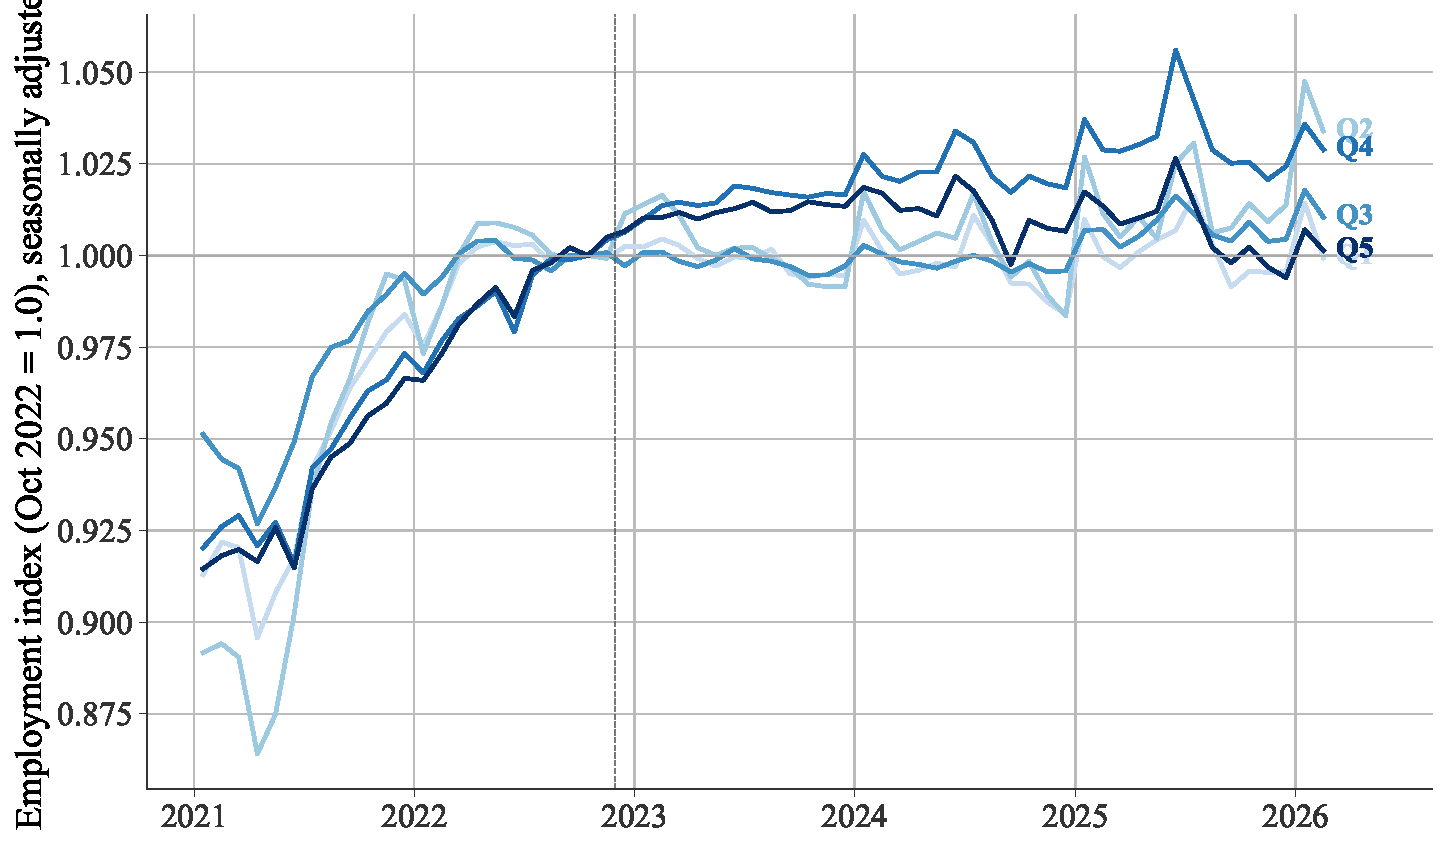
\includegraphics[width=0.85\textwidth]{../analysis/output/figures/figure_emp_byexposure_sa.pdf}
  \caption{Employment by AI-exposure quintile, all ages 21--60, private sector, seasonally adjusted.}
  \label{fig:byexposure_sa}
  \begin{minipage}{\textwidth}\footnotesize\textit{Notes:} Private-sector headcount pooled over ages 21--60, seasonally adjusted by removing fixed calendar-month factors, estimated over 2021--2024 as the average log-deviation from a centred $2\times12$ moving-average trend, indexed to October 2022 = 1. Occupations are ranked by the Eloundou et al.\ GPT-4 exposure score. Q1 (lightest) = least exposed; Q5 (darkest) = most exposed. This is the paper analog of the kiindeksen.no headline ``Sysselsetting etter KI-eksponering'' figure. The raw (unadjusted) series is Appendix Figure~\ref{fig:byexposure_raw}.\end{minipage}
\end{figure}

\subsection{Employment in Selected Occupations}\label{sec:results:occupations}

When we disaggregate by age, there are some signs of canary patterns. We look at four occupations chosen for their AI relevance, the case studies shown on the companion dashboard: software developers and customer service agents, both highly exposed to AI and emphasized by \citet{brynjolfsson2025}, and electricians and home health aides, two low-exposure occupations that serve as a benchmark.\footnote{STYRK-08 codes, code-compatible with overlapping ISCO-08 unit groups for these occupations: software developers 2512--2514 and 2519; customer service agents 4222; electricians 7411; home health aides 5322.} The four differ sharply in measured exposure: software developers and customer service agents are in the top Eloundou quintile and also rank high on the Handa et al.\ usage and automation measures, whereas electricians and home health aides fall in the bottom quintiles on all three measures, so the contrast does not depend on which exposure measure one uses.

Figure~\ref{fig:occupations_by_age} plots seasonally adjusted private-sector employment (headcount) by decade age group, indexed to October 2022. In software development, all age groups were growing before November 2022. Afterwards, 31--40 and 51--60 are still rising, while 41--50 flattens out and the 21--30 group declines rapidly. Customer service agents show a milder version of the same shape, the youngest ending near the baseline while older groups end higher. The two low-exposure occupations show no young-worker decline: electricians aged 21--30 end close to the baseline and home health aides grow across every age group, the youngest most of all.

In the high-exposure occupations, the youngest workers lose ground relative to older workers, the case-study pattern reported in \citet{brynjolfsson2025}, while the low-exposure occupations show no such gap. Section~\ref{sec:results:agequintile} incorporates all occupations systematically and finds that the young-worker decline does not generalize across the exposure distribution.

\begin{figure}[tp]
  \centering
  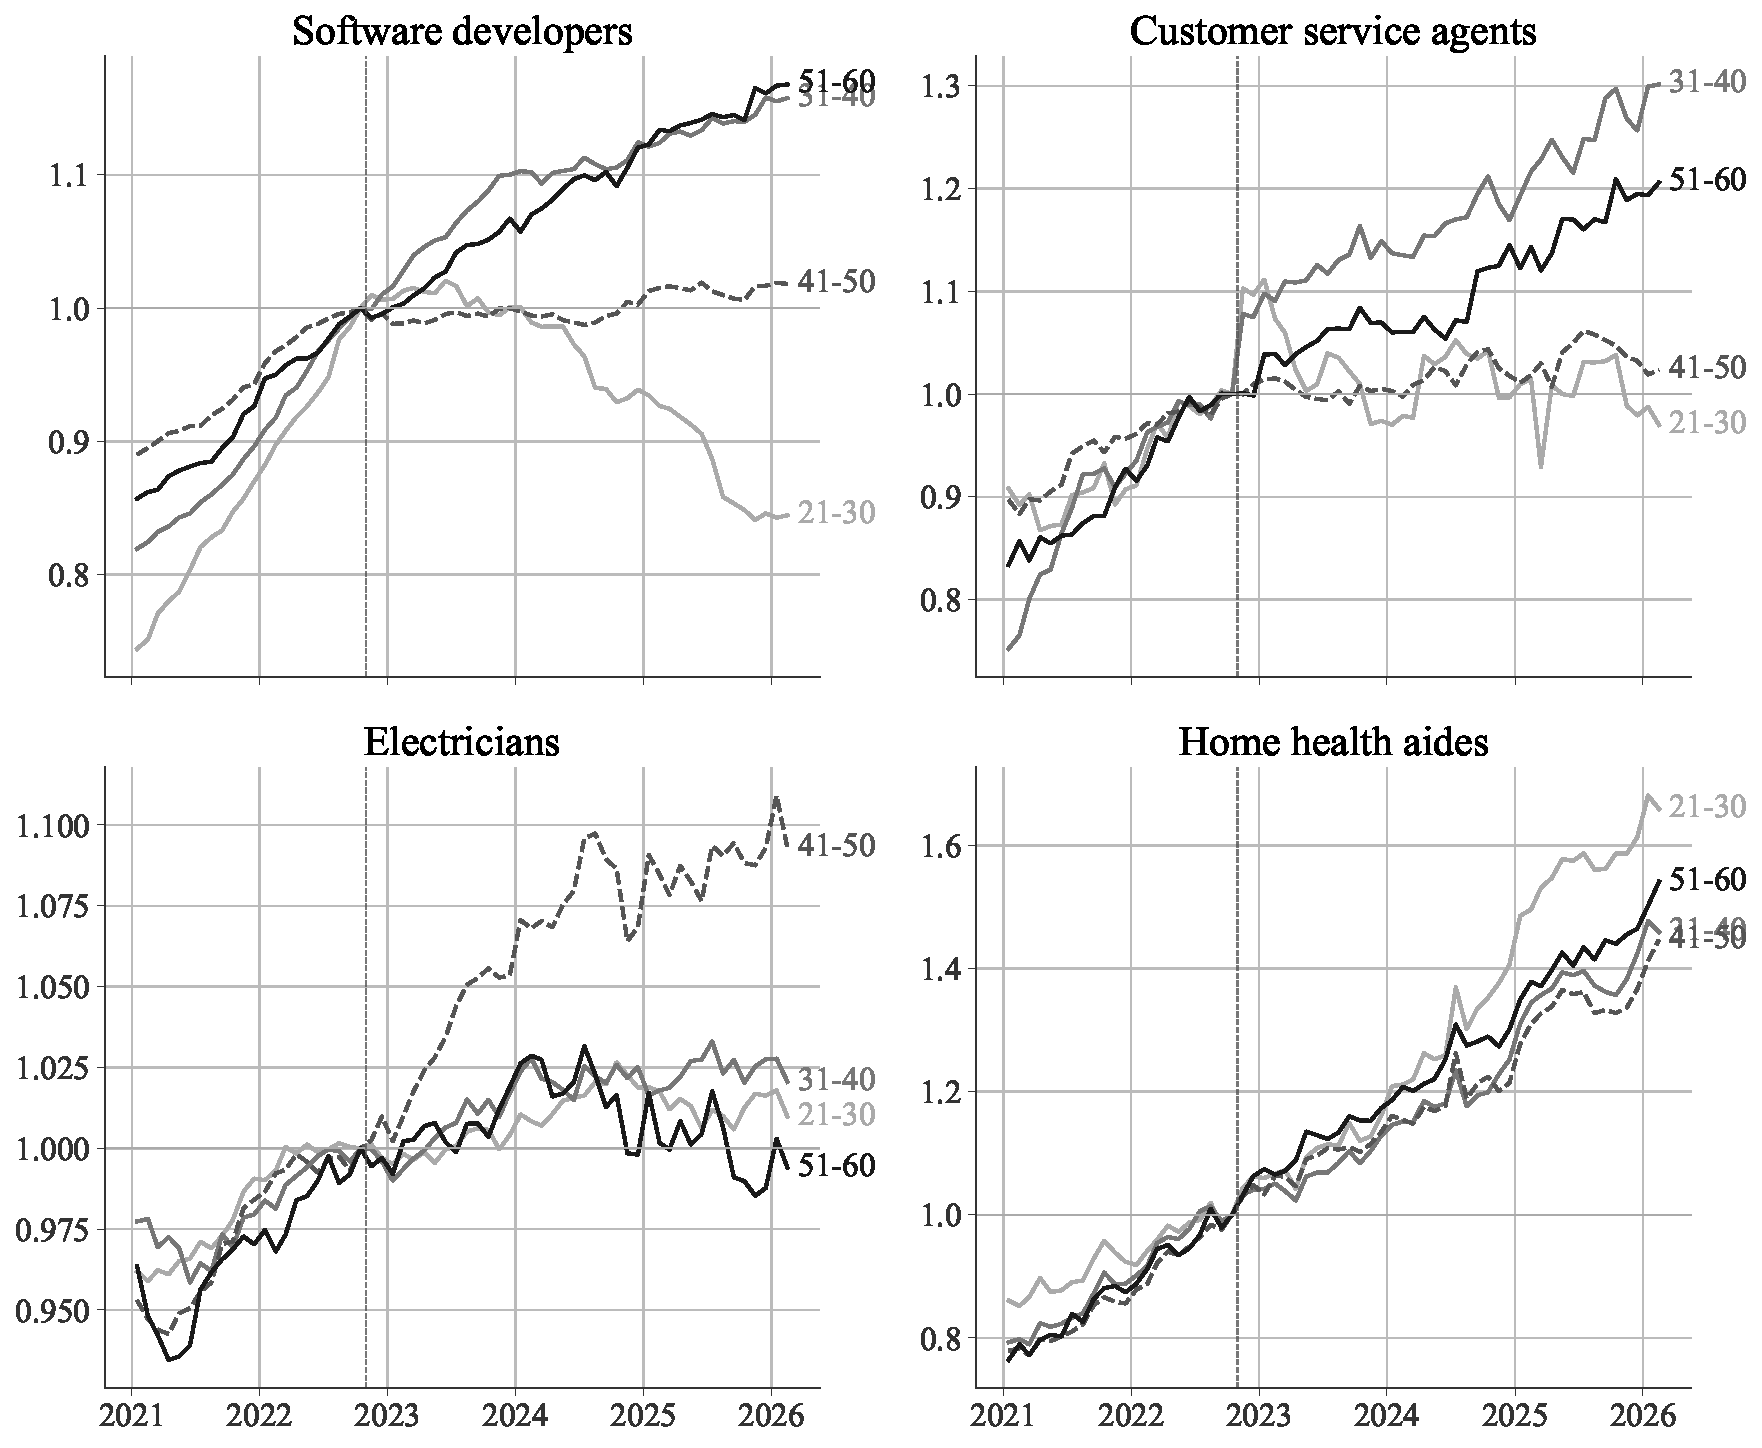
\includegraphics[width=\textwidth]{../analysis/output/figures/figure_occupations_by_age_sa.pdf}
  \caption{Employment in selected occupations, by decade age group, seasonally adjusted.}
  \label{fig:occupations_by_age}
  \begin{minipage}{\textwidth}\footnotesize\textit{Notes:} Private-sector headcount, seasonally adjusted by removing fixed calendar-month factors, estimated over 2021--2024 as the average log-deviation from a centred $2\times12$ moving-average trend, indexed to October 2022 = 1. Panels show the kiindeksen.no case-study occupations: software developers (STYRK-08 2512--2514, 2519) and customer service agents (4222), both high-exposure, and electricians (7411) and home health aides (5322), both low-exposure. The vertical dashed line marks the November 2022 ChatGPT release.\end{minipage}
\end{figure}

\subsection{Employment by Age and Exposure Quintile}\label{sec:results:agequintile}

The selected-occupation pattern does not generalize. Ranking all occupations by exposure and following each quintile separately within each decade age group, the most-exposed occupations do not systematically lose ground among the youngest workers. Each of the four panels in Figure~\ref{fig:age_by_quintile} is one decade age group, with quintile lines from light blue (Q1, least exposed) to dark blue (Q5, most exposed) and a red line for the overall age-group trend.

In the 21--30 group the Q5 series tracks Q1 after the ChatGPT release, so the broader ranking does not reproduce the decline seen in the selected occupations. Among the older groups the Q5 series runs above Q1 at 31--40, ends a few points below at 41--50, and shows no clear separation at 51--60; these older movements are smaller than the pre-period swings discussed in Section~\ref{sec:regression:robust}. The raw panels are in Appendix Figure~\ref{fig:age_by_quintile_raw}.

\begin{figure}[tp]
  \centering
  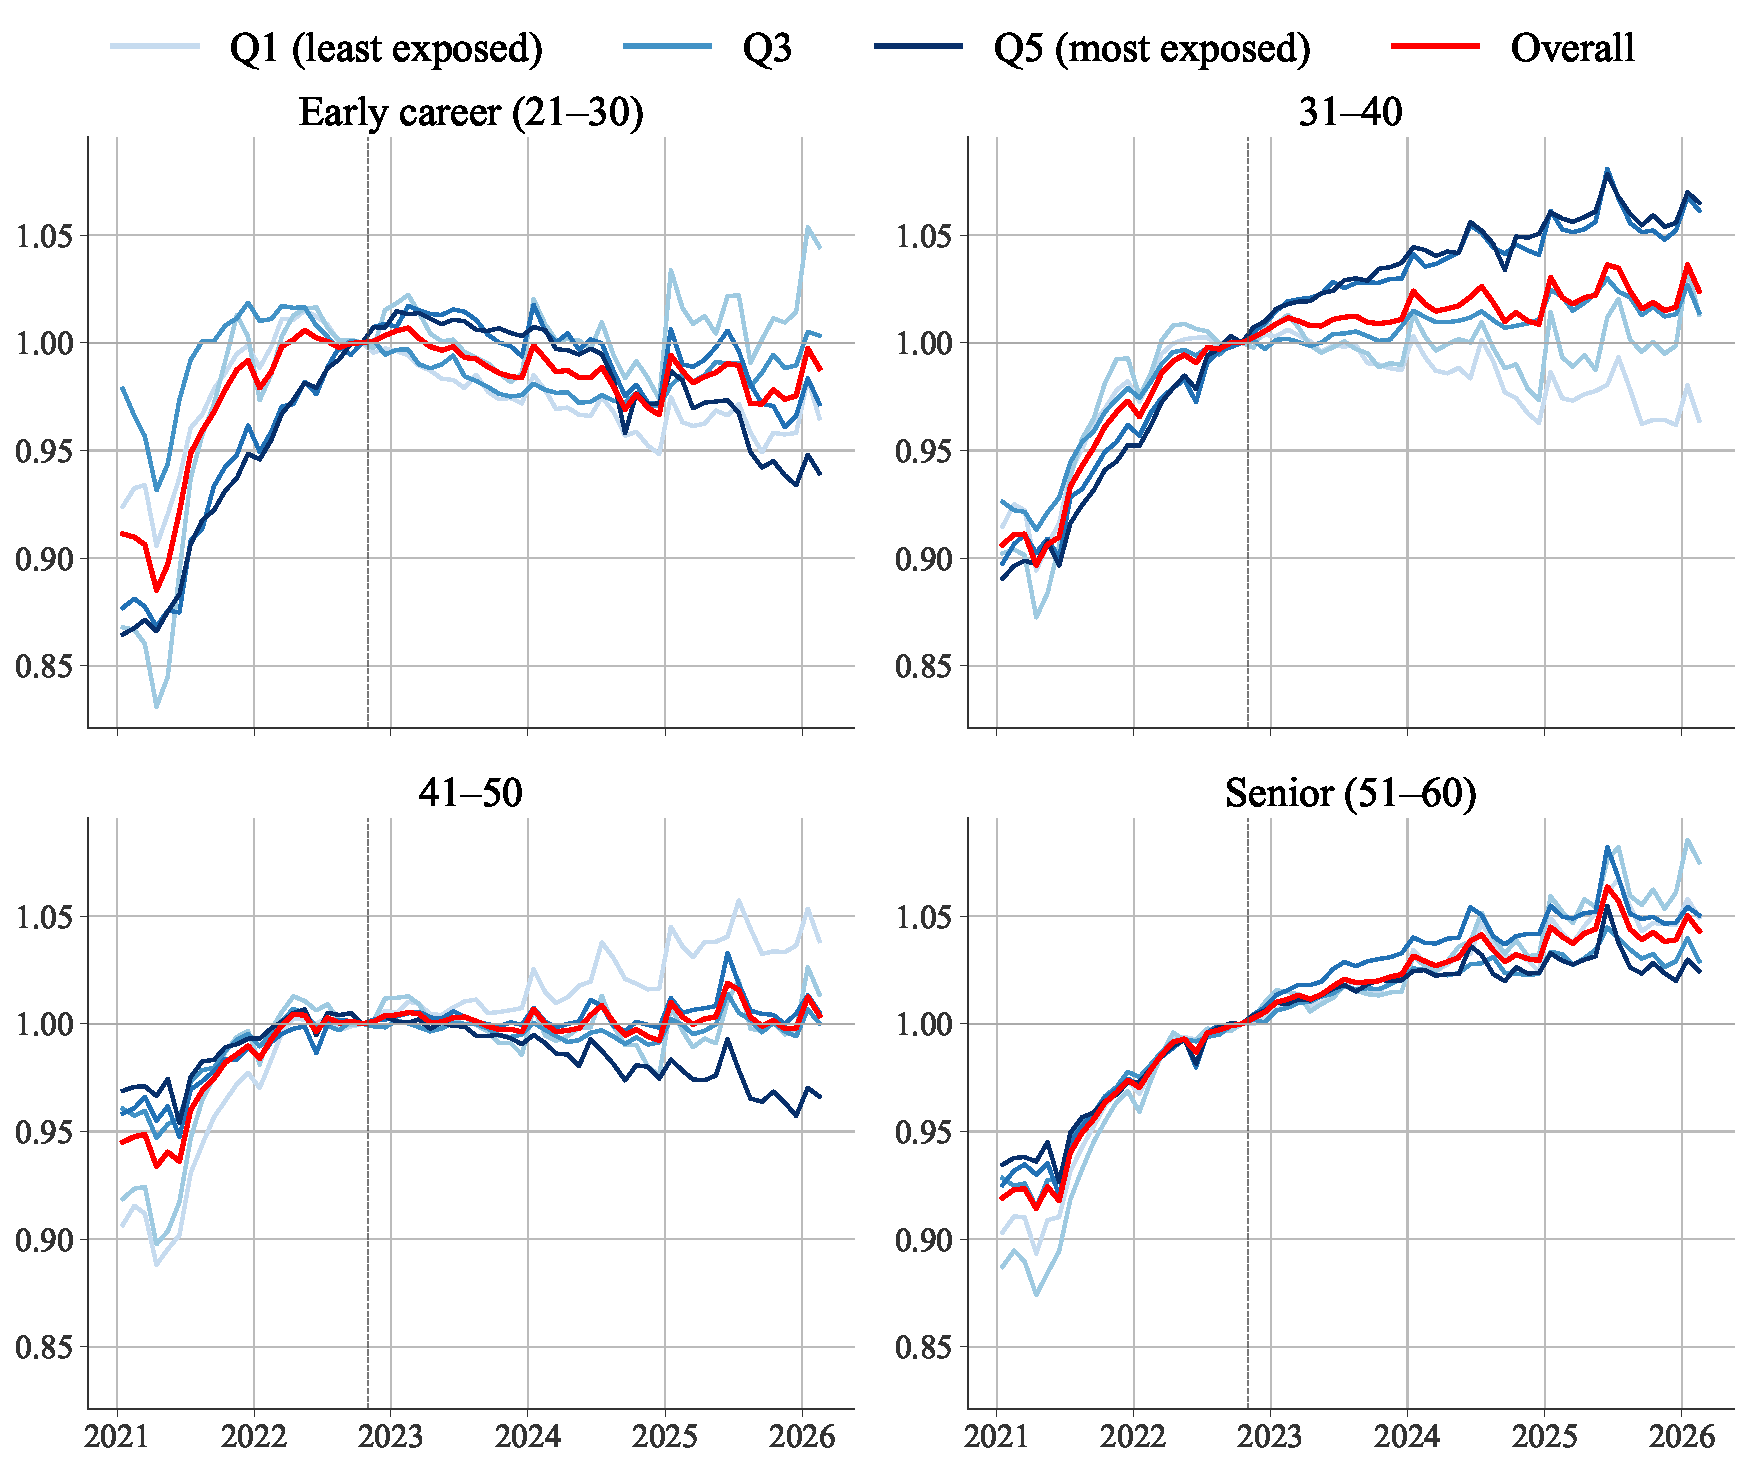
\includegraphics[width=\textwidth]{../analysis/output/figures/figure_emp_decade_private_sa.pdf}
  \caption{Employment by AI-exposure quintile and decade age group, private sector, seasonally adjusted.}
  \label{fig:age_by_quintile}
  \begin{minipage}{\textwidth}\footnotesize\textit{Notes:} Private-sector headcount, seasonally adjusted by removing fixed calendar-month factors, estimated over 2021--2024 as the average log-deviation from a centred $2\times12$ moving-average trend, indexed to October 2022 = 1. Occupations are ranked by the Eloundou et al.\ GPT-4 exposure score. Q1 (lightest) = least exposed; Q5 (darkest) = most exposed. Red line = overall age-group trend. Vertical dashed line marks the November 2022 ChatGPT release. The raw (unadjusted) per-capita series is Appendix Figure~\ref{fig:age_by_quintile_raw}.\end{minipage}
\end{figure}

\subsection{Automation versus Augmentation}\label{sec:results:auto_aug}

We split AI exposure into the two using the \citet{handa2025} decomposition of observed Claude.ai usage into directive task delegation (automation) and collaborative iteration (augmentation), which likely carry opposite labor-market implications. We rank occupations separately by each share, and plot seasonally adjusted employment by quintile within each age group.

Ranking the youngest workers by automation share gives a modest negative gradient (Figure~\ref{fig:handa_auto_sa}); ranking them by augmentation share gives no gradient at all (Figure~\ref{fig:handa_aug_sa}). This pattern is more consistent with automation than with augmentation, though the Handa classification captures conversation mode rather than what workers do on the job, so an occupation scored as automation-exposed may in practice use AI for augmentation. From the second half of 2025, the most-exposed automation quintile begins to separate more visibly among the youngest workers. The raw automation and augmentation panels are in Appendix Figures~\ref{fig:age_by_quintile_handa_auto} and~\ref{fig:age_by_quintile_handa_aug}.

\begin{figure}[tp]
  \centering
  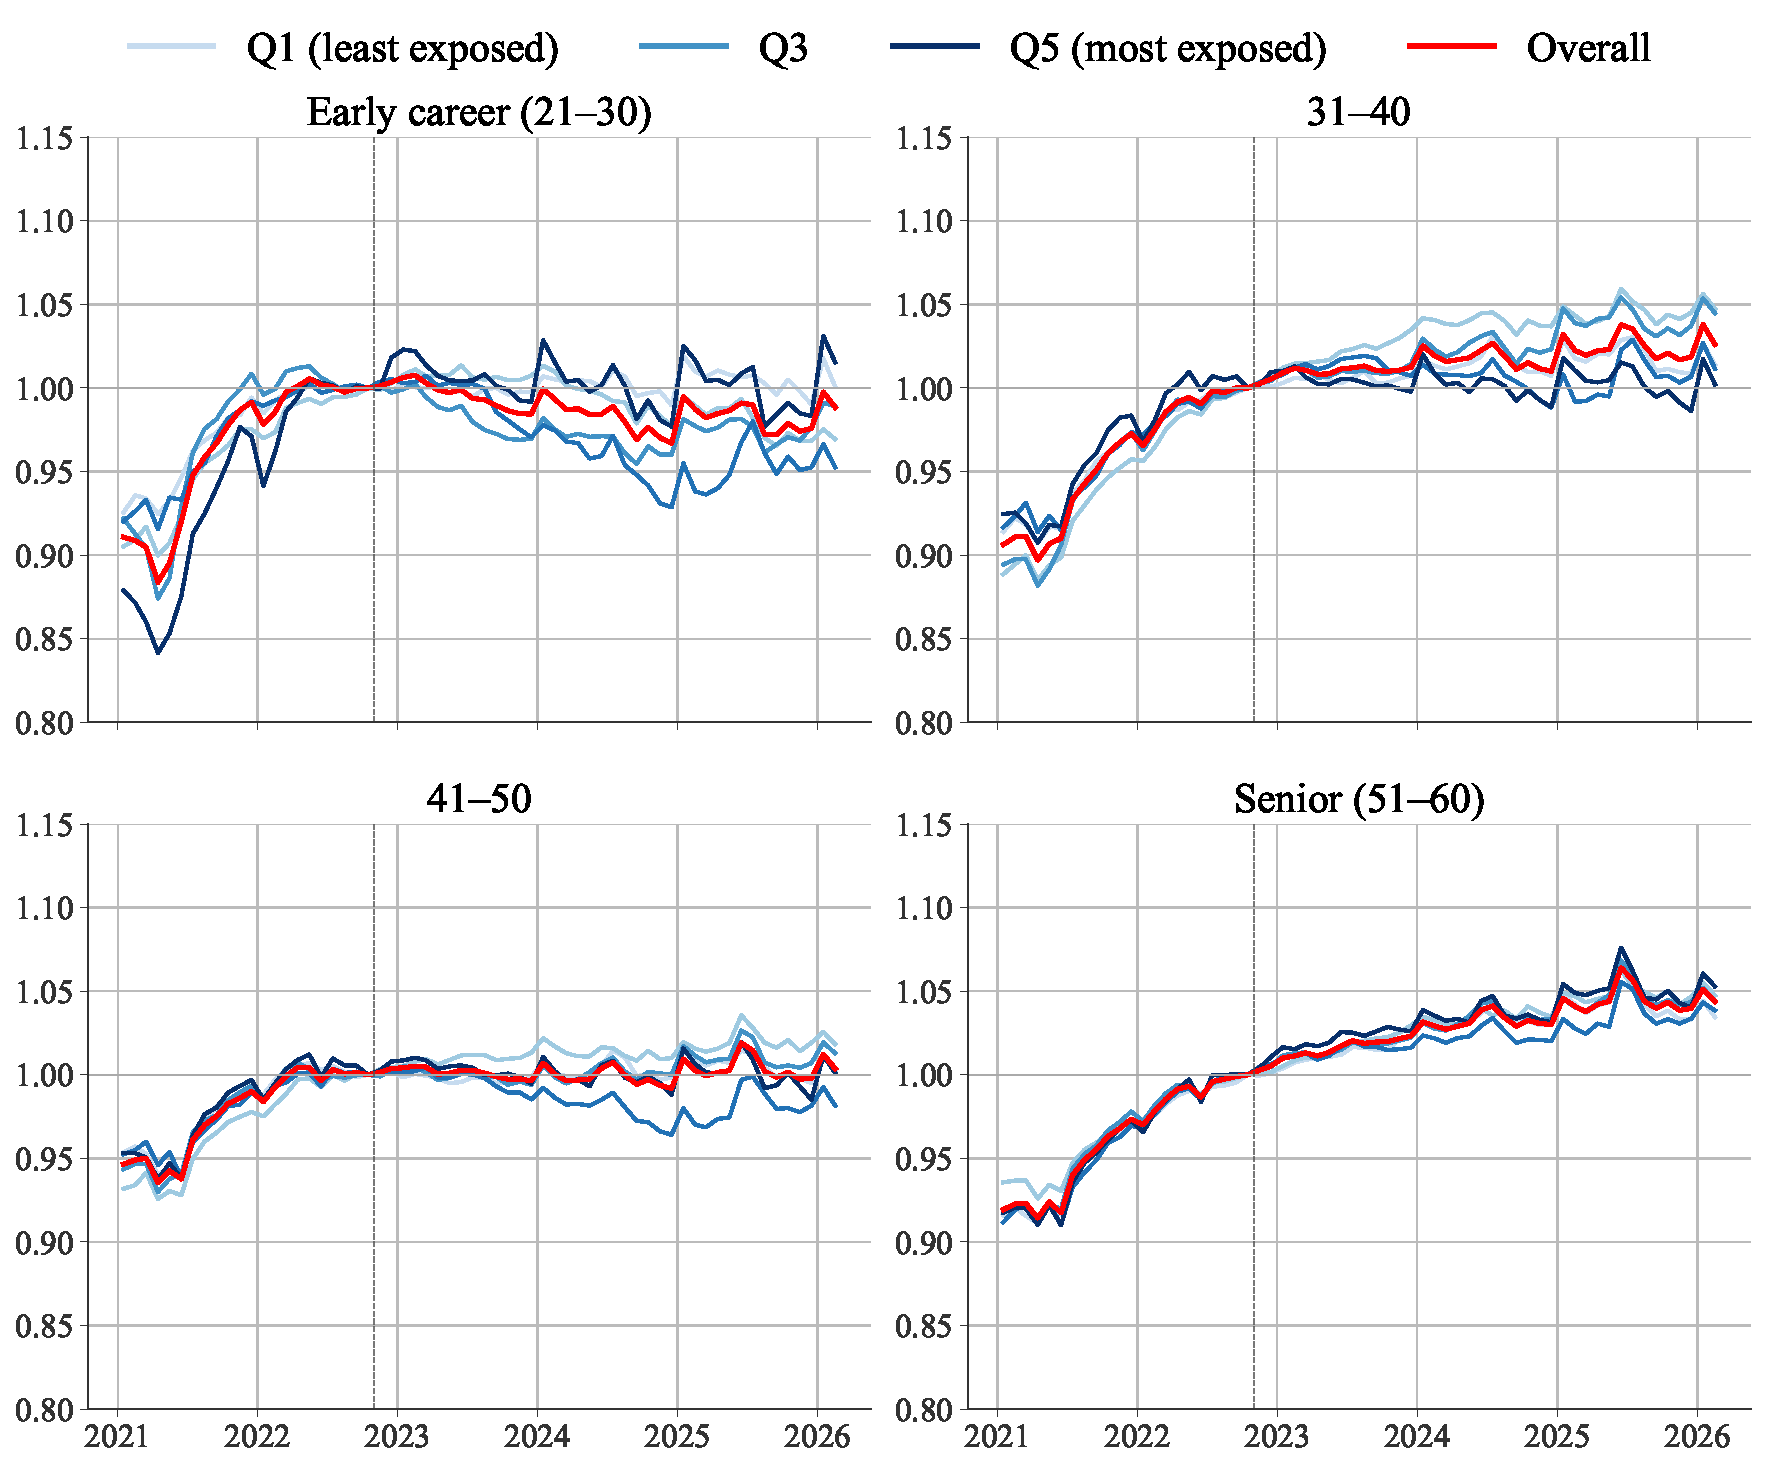
\includegraphics[width=\textwidth]{../analysis/output/figures/figure_age_by_quintile_handa_auto_sa.pdf}
  \caption{Employment by Handa et al.\ automation-exposure quintile and decade age group, private sector, seasonally adjusted.}
  \label{fig:handa_auto_sa}
  \begin{minipage}{\textwidth}\footnotesize\textit{Notes:} Private-sector headcount, seasonally adjusted by removing fixed calendar-month factors, estimated over 2021--2024 as the average log-deviation from a centred $2\times12$ moving-average trend, indexed to October 2022 = 1. Occupations are ranked by the Handa et al.\ automation share. Q1 (lightest) = least exposed; Q5 (darkest) = most exposed. The raw series is Appendix Figure~\ref{fig:age_by_quintile_handa_auto}.\end{minipage}
\end{figure}

\begin{figure}[tp]
  \centering
  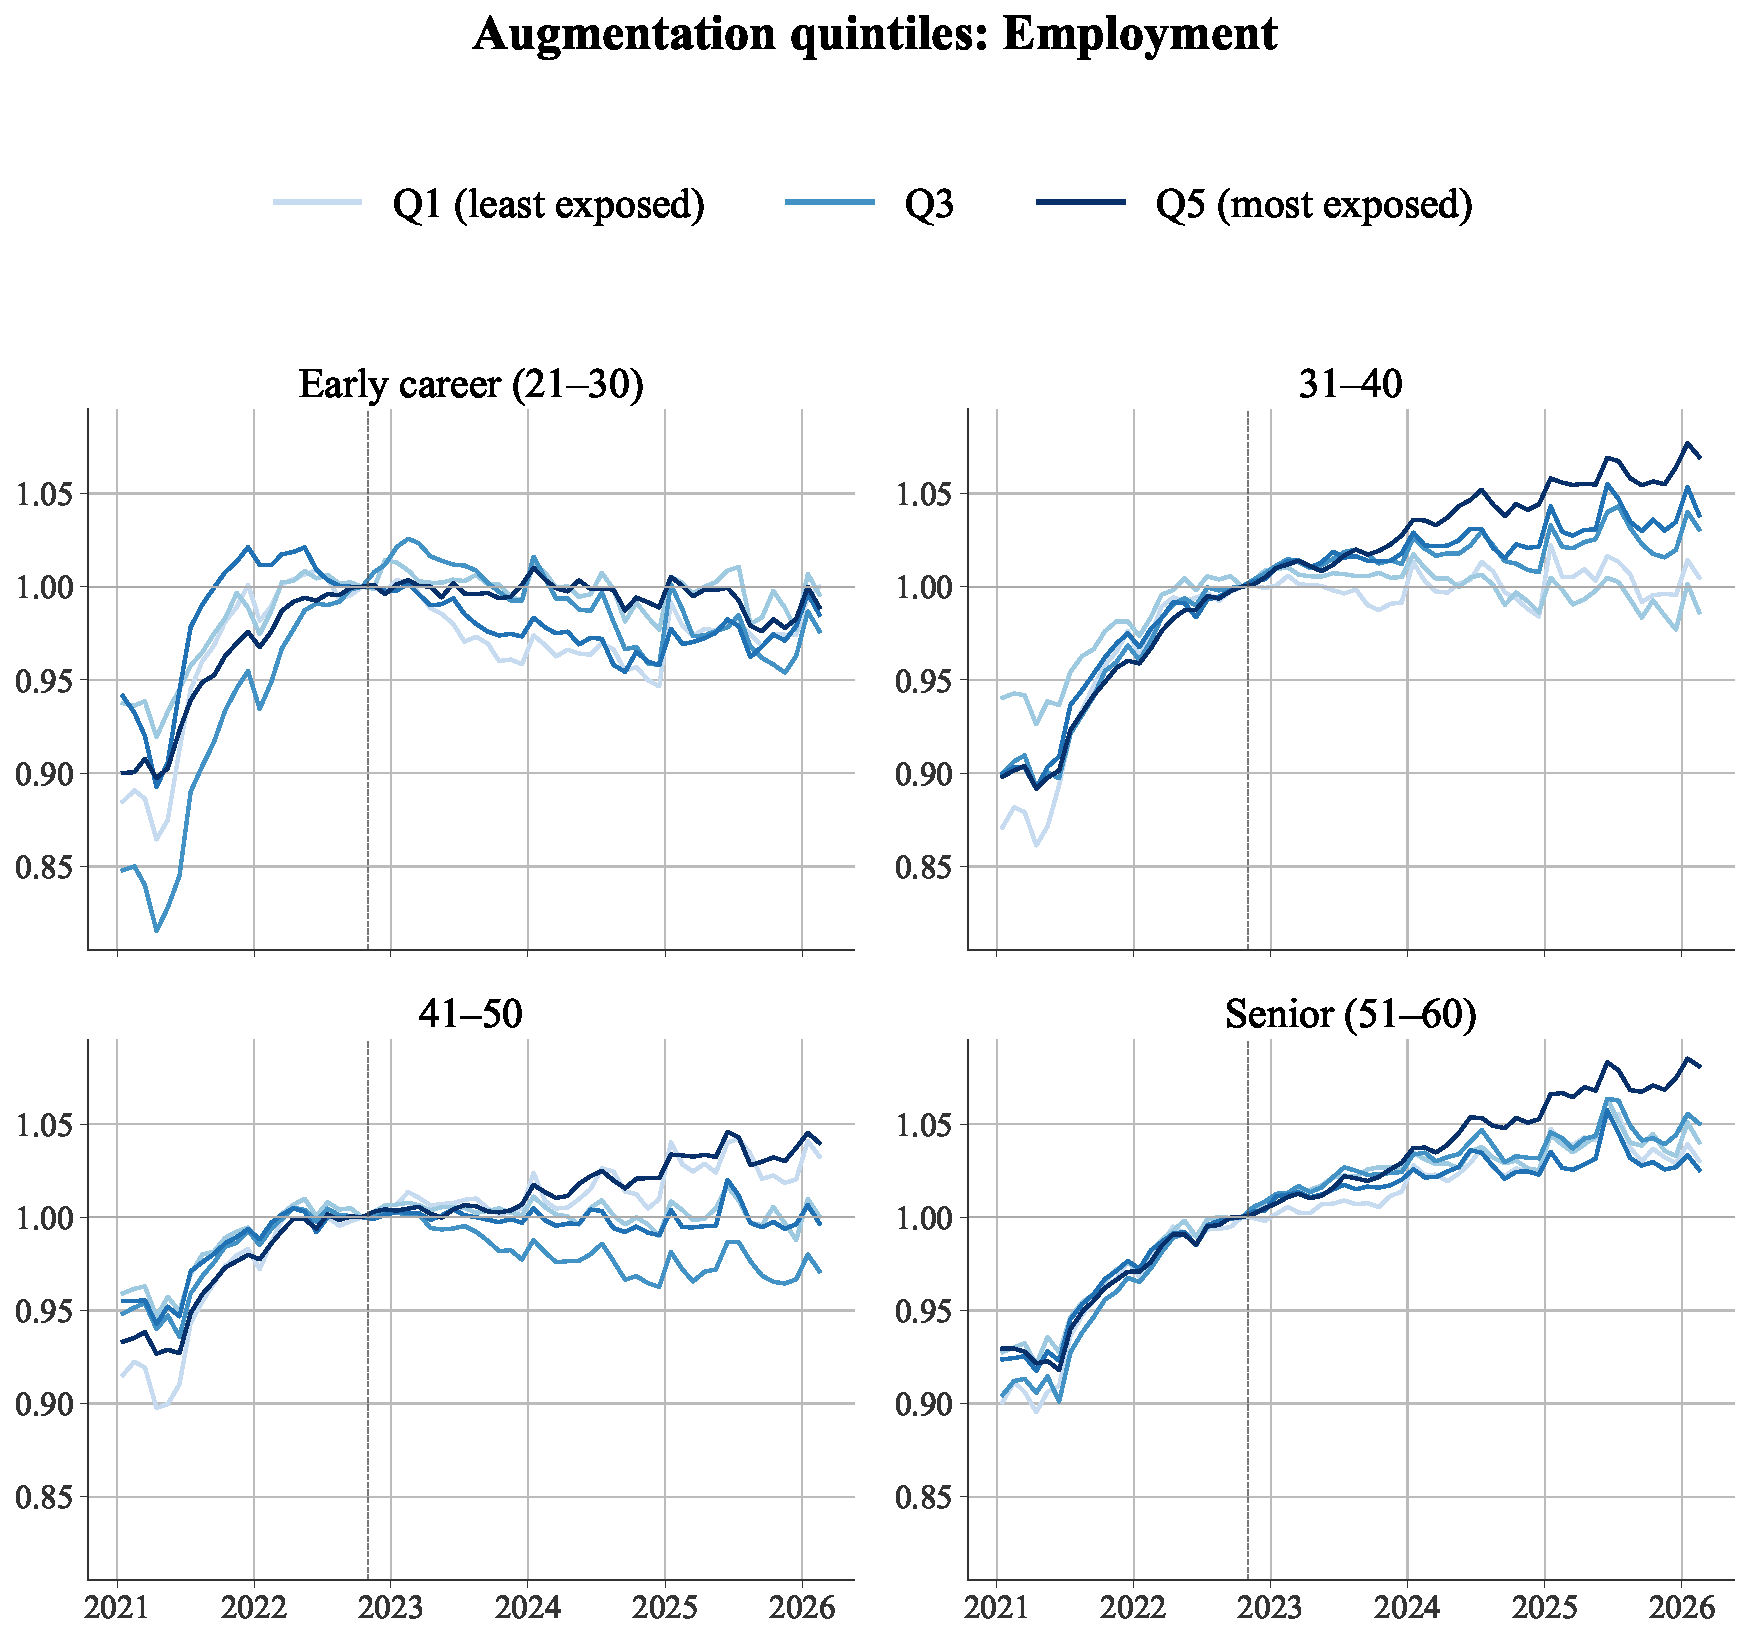
\includegraphics[width=\textwidth]{../analysis/output/figures/figure_age_by_quintile_handa_aug_sa.pdf}
  \caption{Employment by Handa et al.\ augmentation-exposure quintile and decade age group, private sector, seasonally adjusted.}
  \label{fig:handa_aug_sa}
  \begin{minipage}{\textwidth}\footnotesize\textit{Notes:} Private-sector headcount, seasonally adjusted by removing fixed calendar-month factors, estimated over 2021--2024 as the average log-deviation from a centred $2\times12$ moving-average trend, indexed to October 2022 = 1. Occupations are ranked by the Handa et al.\ augmentation share. Q1 (lightest) = least exposed; Q5 (darkest) = most exposed. The raw series is Appendix Figure~\ref{fig:age_by_quintile_handa_aug}.\end{minipage}
\end{figure}

\subsection{Secondary outcomes}\label{sec:results:extensions}

Earnings are the most telling of the secondary outcomes, because a labor-demand shift could in principle show up on the price margin rather than the quantity margin. Cash earnings show no divergence by exposure quintile (Appendix Figure~\ref{fig:kontantlonn_by_quintile}); the wage plots are dominated by seasonal patterns (June holiday pay, December bonuses), and the within-firm difference-in-differences estimates (Table~\ref{tab:did_firmfe}) show no large earnings movement. \citet{brynjolfsson2025} and \citet{humlum2026} likewise find no wage divergence over a similar horizon in the US and Denmark. Norway's two-tier bargaining system \citep{bhuller2022}, with sectoral wage floors and strong employment protection, makes the quantity margin the more likely site of adjustment. New hires also show no comparable exposure gradient (Table~\ref{tab:did_firmfe} and Appendix Figure~\ref{fig:nyjobb_by_quintile}). Raw series for overtime hours is shown in the appendix (Appendix Figure~\ref{fig:overtid_by_quintile}). 


% =============================================================================
\section{Regression Analysis}\label{sec:regression}

\subsection{Quintile Analysis}\label{sec:regression:quintile}

We begin with a compact cross-section of the whole exposure distribution. We measure each occupation's percentage change in employment from its pre-ChatGPT baseline,
\[
\Delta_j \;=\; \frac{\text{emp}_{j,\text{last}} - \text{emp}_{j,\text{Oct }2022}}{\text{emp}_{j,\text{Oct }2022}},
\]
where $\text{emp}_{j,\text{last}}$ is occupation $j$'s seasonally adjusted private-sector headcount in the last month of data (February 2026) and the denominator is its October 2022 level. We regress $\Delta_j$ on exposure-quintile dummies, weighting each occupation by its October 2022 employment so the quintile means reproduce the headcount aggregation used by the companion index \citep{kiindeksen2026}, with heteroskedasticity-robust standard errors across occupations.

Table~\ref{tab:quintile_yagan} reports the result. The top row is the employment-weighted mean change in each quintile; the bottom row is the double difference relative to Q1, the least-exposed quintile, which serves as the base. The most-exposed quintile has not grown differently from the least-exposed since ChatGPT: the Q5$-$Q1 double difference is small and statistically insignificant.

\begin{table}[tp]
  \centering
  \caption{Employment change by AI-exposure quintile, October 2022 to February 2026, all ages 21--60, private sector, seasonally adjusted.}
  \label{tab:quintile_yagan}
  \begin{tabular}{lccccc}
\toprule
 & Q1 & Q2 & Q3 & Q4 & Q5 \\
\midrule
Average change (\%) & -0.63 & +2.94 & +0.95 & +2.86 & -0.09 \\
\addlinespace
Difference vs.\ Q1 (\%) & --- & +3.57 & +1.59 & +3.49 & +0.54 \\
 &  & (5.36) & (2.67) & (2.15) & (2.42) \\
\midrule
Occupations & \multicolumn{5}{c}{374} \\
\bottomrule
\end{tabular}

  \begin{minipage}{\textwidth}\footnotesize\textit{Notes:} Percentage change in employment $\Delta_j = (\text{emp}_{j,\text{Feb }2026}-\text{emp}_{j,\text{Oct }2022})/\text{emp}_{j,\text{Oct }2022}$ for each occupation's seasonally adjusted private-sector headcount, pooled over ages 21--60. The top row is the employment-weighted mean change by exposure quintile (occupations ranked by the Eloundou et al.\ GPT-4 score); the bottom row is the double difference relative to Q1 (the base quintile, hence no entry), with heteroskedasticity-robust standard errors in parentheses. Occupations are weighted by October 2022 employment, reproducing the headcount aggregation of the companion index. $^{*}$, $^{**}$, $^{***}$ denote significance at the 10, 5, and 1 percent levels.\end{minipage}
\end{table}

\subsection{Age Heterogeneity}\label{sec:regression:age}

The cross-section pools all ages; we now let the exposure gradient differ by decade age group, since the youngest workers are the margin of interest. The Poisson event study on the worker counts is our baseline specification, and the percentage-change-in-employment outcome computed within age groups gives the same qualitative picture.

The cell-level microdata are tabulated at the (occupation $\times$ age group $\times$ month) level. We estimate
\[
\log E[\text{count}_{j,a,t}] = \alpha_{j} + \beta_{t} + \gamma_{q,k},
\]
separately per decade age group~$a$ in the private sector, where $j$ indexes occupations and $q(j)$ is the Eloundou GPT-4 quintile of occupation~$j$. The occupation fixed effect absorbs the permanent employment level of each occupation; the month fixed effect absorbs the aggregate time path of the age cohort. Standard errors are clustered at occupation, with Q1 and $k=-1$ (October 2022) as the reference.

Figure~\ref{fig:microdata_poisson_grid} reports the resulting $\gamma_{q,k}$ for $q\in\{2,3,4,5\}$ across the four decade age groups, in log points. The path matches the indexed series in Figure~\ref{fig:age_by_quintile}. At 41--50 the Q5 path turns negative after October 2022, reaches about $-0.08$ log points by mid-2025, and ends near $-0.03$ by early 2026. At 21--30 the Q5 path is noisy and ends near zero; at 31--40 it rises to about $+0.15$; at 51--60 it stays near zero.

\begin{figure}[tp]
  \centering
  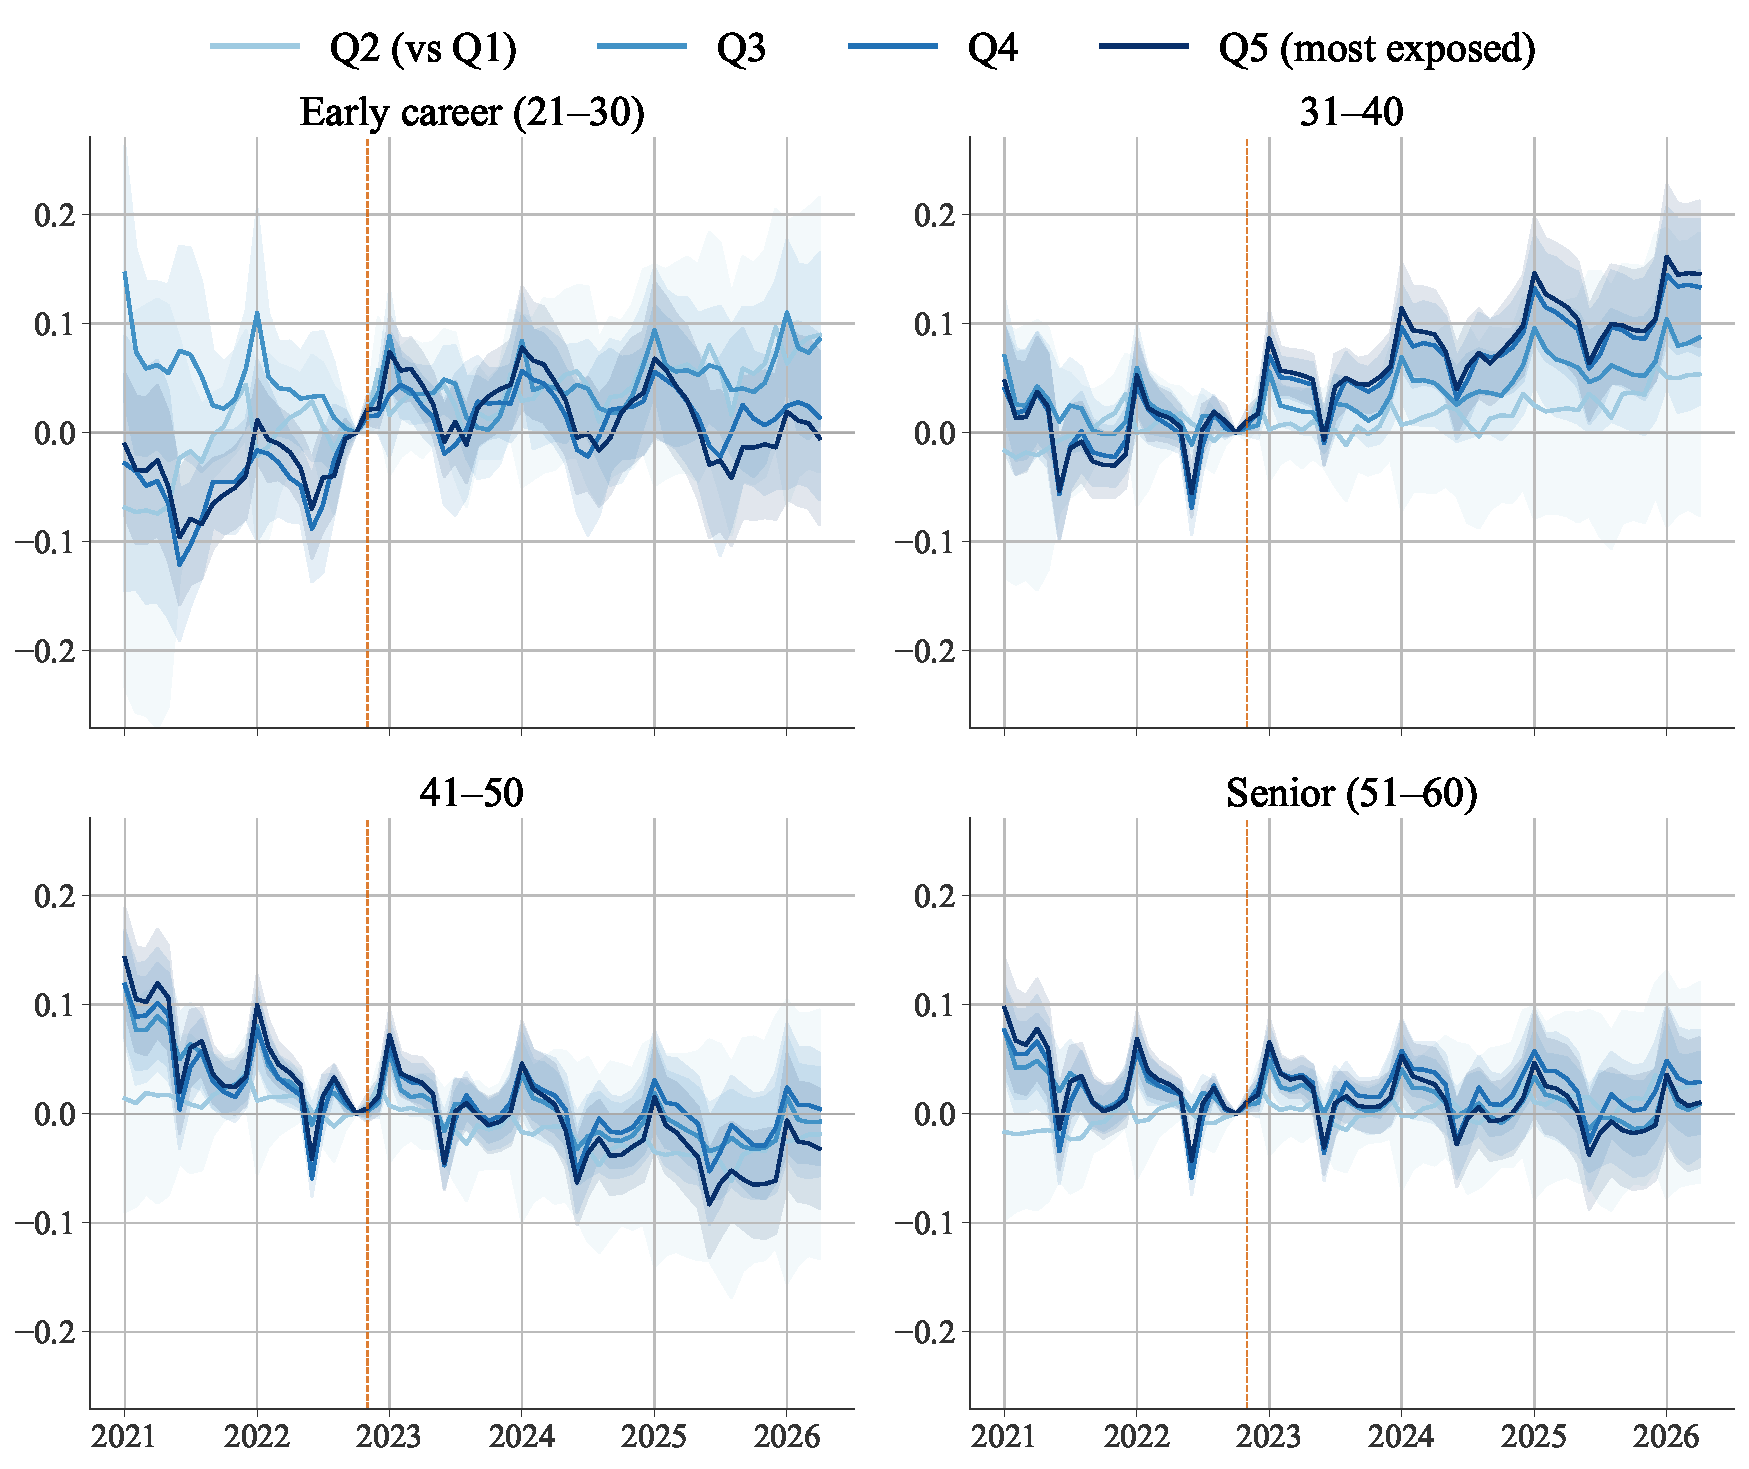
\includegraphics[width=\textwidth]{../analysis/output/figures/figure_microdata_poisson_es_grid.pdf}
  \caption{Poisson event-study coefficients by AI-exposure quintile and decade age group, private sector.}
  \begin{minipage}{\textwidth}\footnotesize\textit{Notes:} Coefficients $\gamma_{q,k}$ for $q\in\{2,\dots,5\}$ relative to $q=1$, in log points. Cell-level microdata.no aggregates (occupation\,$\times$\,age\,$\times$\,month), private sector; fixed effects for occupation and month. Sample 2021m1--2026m2. Shaded bands: 95\% confidence intervals clustered at occupation. Reference: October 2022. Dashed line marks the November 2022 ChatGPT release.\end{minipage}
  \label{fig:microdata_poisson_grid}
\end{figure}

Table~\ref{tab:did_cell} collapses the event study into a post-versus-pre difference-in-differences by age group, for employment and new hires. For the youngest workers the most-exposed quintiles are not statistically distinguishable from Q1, and new hires show no systematic gradient in any age group. Among the older groups the employment estimate is positive at 31--40 (Q5 about $+0.078$ log points, $p<0.01$) and a small, insignificant negative at 41--50 ($-0.015$). The percentage-change-in-employment outcome computed within each age group gives the same signs. Because pre-trends differ across these groups (Section~\ref{sec:regression:robust}), we read these post-period summaries as descriptive: an insignificant estimate is an absence of a detectable gradient, not evidence that exposure has no effect.

\begin{table}[tp]
  \centering
  \caption{Cell-level difference-in-differences by AI-exposure quintile and decade age group, private sector.}
  \label{tab:did_cell}
  \begin{tabular}{lcccc}
\toprule
 & Early career & 31--40 & 41--50 & Senior \\
 & (21--30) &  &  & (51--60) \\
 & (1) & (2) & (3) & (4) \\
\midrule
\multicolumn{5}{l}{\textit{Panel A. Employment (Poisson)}} \\
Q2 $\times$ Post & 0.0428 & 0.0181 & -0.0206 & 0.0080 \\
 & (0.0341) & (0.0357) & (0.0339) & (0.0268) \\
Q3 $\times$ Post & 0.0449$^{**}$ & 0.0432$^{***}$ & -0.0049 & 0.0102 \\
 & (0.0204) & (0.0167) & (0.0153) & (0.0135) \\
Q4 $\times$ Post & 0.0193 & 0.0707$^{***}$ & 0.0000 & 0.0216 \\
 & (0.0203) & (0.0169) & (0.0154) & (0.0134) \\
Q5 $\times$ Post & 0.0215 & 0.0783$^{***}$ & -0.0146 & 0.0103 \\
 & (0.0220) & (0.0186) & (0.0169) & (0.0166) \\
\addlinespace
\multicolumn{5}{l}{\textit{Panel B. New hires (Poisson)}} \\
Q2 $\times$ Post & 0.1247 & 0.2475$^{**}$ & 0.1836 & 0.2422$^{*}$ \\
 & (0.0810) & (0.1223) & (0.1247) & (0.1452) \\
Q3 $\times$ Post & 0.1158 & 0.1775$^{*}$ & 0.0999 & 0.0657 \\
 & (0.0740) & (0.1019) & (0.1100) & (0.1129) \\
Q4 $\times$ Post & 0.0713 & 0.1303 & 0.0591 & -0.0043 \\
 & (0.0770) & (0.1024) & (0.1074) & (0.1190) \\
Q5 $\times$ Post & -0.0424 & 0.0160 & -0.0116 & 0.0200 \\
 & (0.0845) & (0.1054) & (0.1104) & (0.1122) \\
\midrule
Occupations & 393 & 391 & 393 & 392 \\
Observations (count) & 24,366 & 24,242 & 24,366 & 24,304 \\
\bottomrule
\end{tabular}

  \begin{minipage}{\textwidth}\footnotesize\textit{Notes:} Each entry is the post-October-2022 change in the indicated quintile relative to Q1 (least exposed), by decade age group. Employment and new hires are Poisson. Occupation and month fixed effects; standard errors clustered by occupation. Sample 2021m1--2026m2. $^{*}$, $^{**}$, $^{***}$ denote $p<0.1$, $0.05$, $0.01$.\end{minipage}
\end{table}


\subsection{Individual-Level Estimates}\label{sec:regression:firmfe}

The cell-level estimates absorb the average employment path of each occupation but do not separate reallocation \emph{within} firms from changes in firm composition. Using the individual-level records, we estimate the within-firm composition design of \citet{brynjolfsson2025},
\[
\log E[\text{count}_{f,q,a,t}] = \alpha_{f,q} + \beta_{f,t} + \gamma_{q,k},
\]
on the panel of firm $f$ $\times$ quintile $q$ $\times$ month $t$ cells, separately per decade age group. Firm-by-quintile and firm-by-month fixed effects absorb the firm's persistent composition and any firm-level demand shock; identification rests on within-firm reallocation across exposure quintiles. Standard errors are clustered at the firm. The sample is private-sector \emph{foretak} with at least 20 workers in the 21--60 age window per month, January 2021 through February 2026.

Figure~\ref{fig:firmfe_poisson_grid} reports the firm-FE $\gamma_{q,k}$. For the youngest workers the Q5 path is noisy and ends slightly positive, so the within-firm comparison, like the cell-level one, does not show the most-exposed quintile penalizing the young. The older groups line up with the cell-level estimates: at 31--40 the Q5 path rises to about $+0.12$, at 41--50 it drifts negative through 2025 and recovers to near zero by early 2026, and at 51--60 it stays near zero. The collapsed within-firm estimates in Table~\ref{tab:did_firmfe} match this reading: the Q5 employment coefficient is not distinguishable from zero at 21--30, positive at 31--40 ($+0.050$, $p<0.01$), marginally negative at 41--50 ($-0.021$, $p<0.1$), and near zero at 51--60. New hires show no systematic exposure gradient.

\begin{figure}[tp]
  \centering
  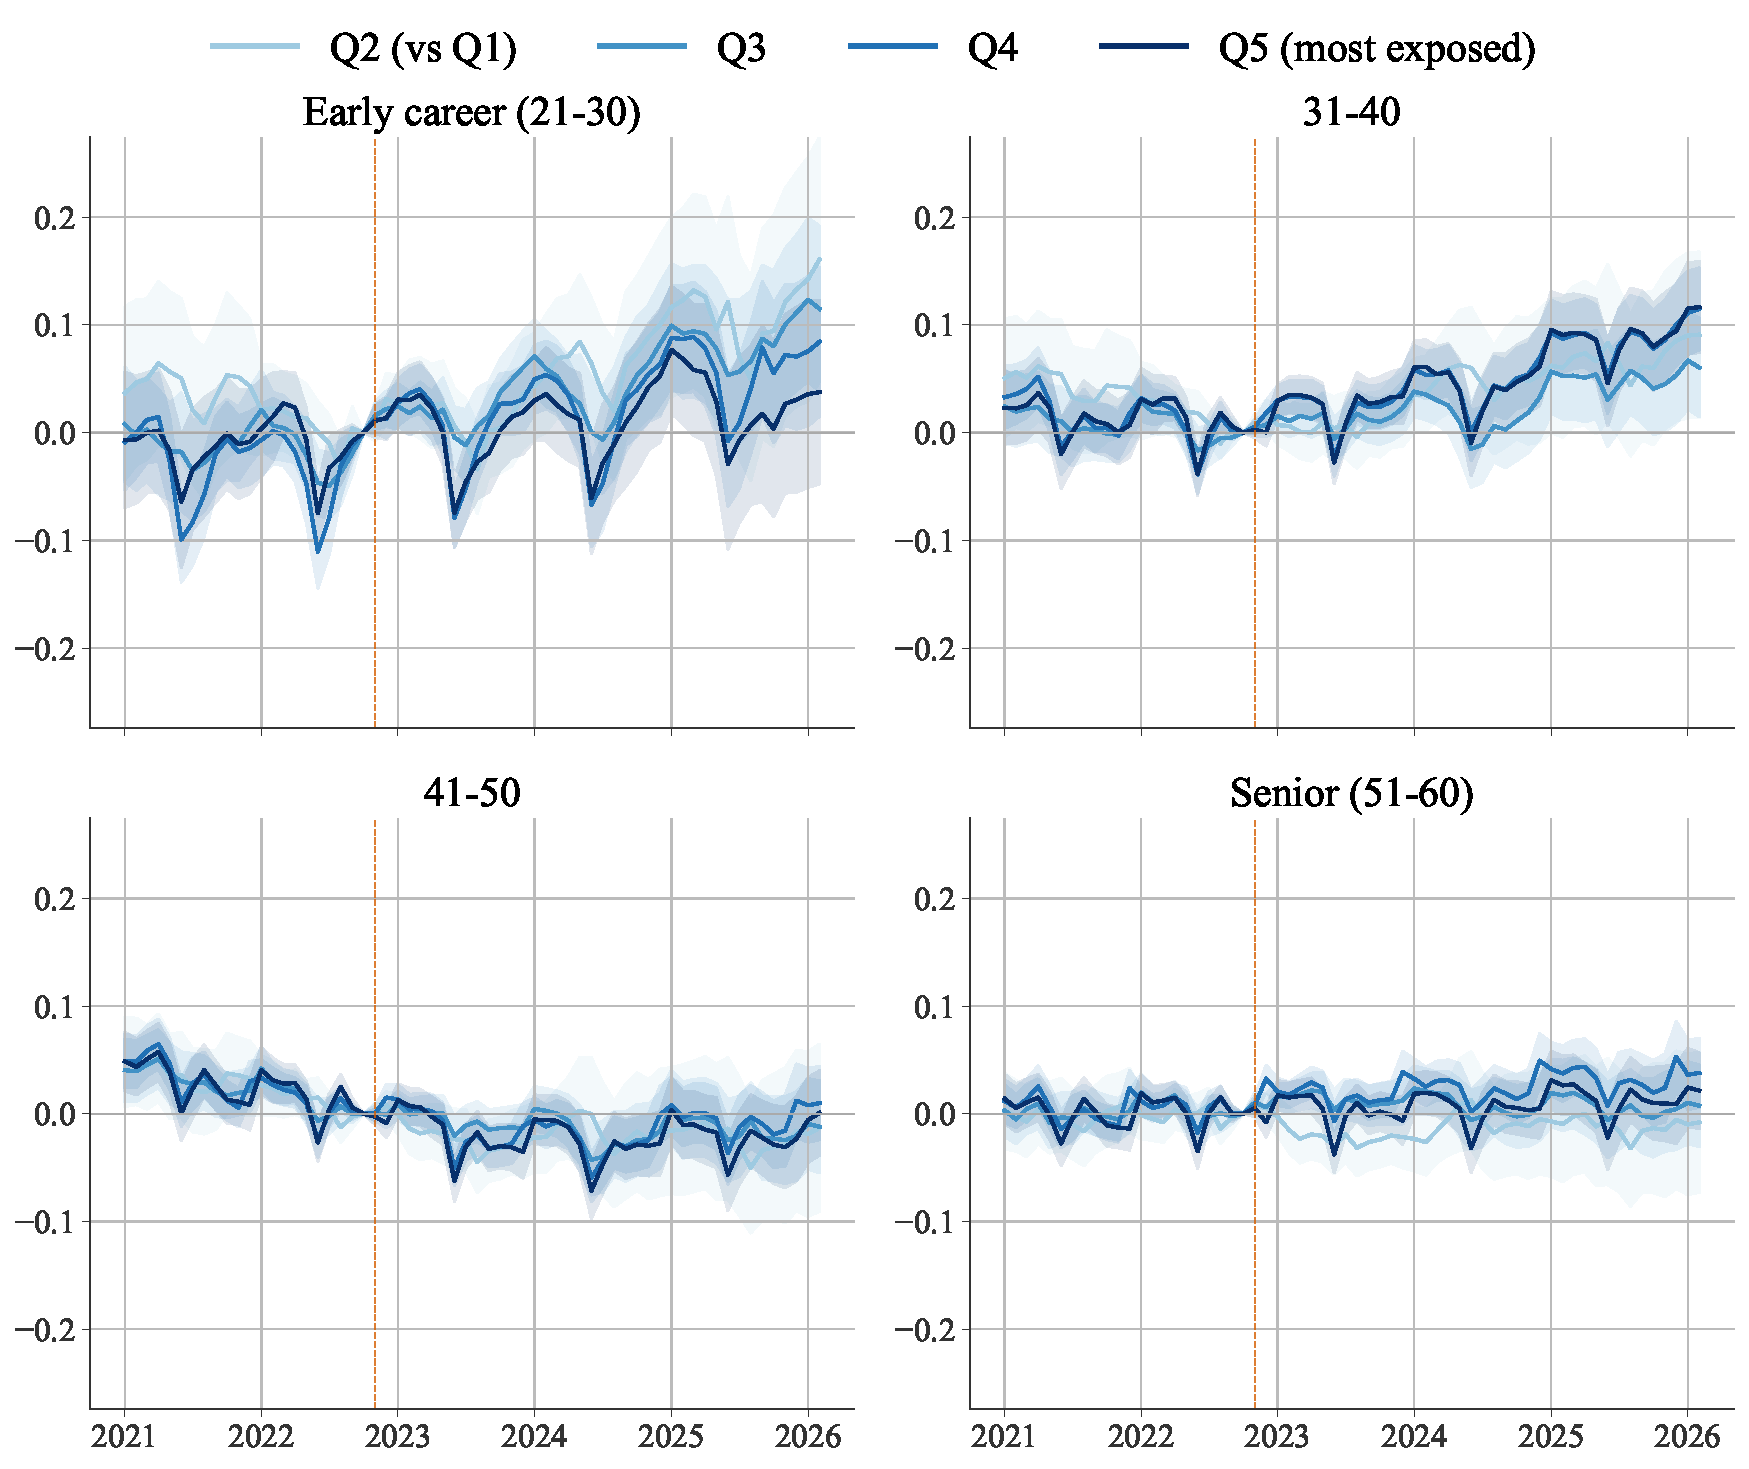
\includegraphics[width=\textwidth]{../analysis/output/figures/figure_firmfe_poisson_es_grid.pdf}
  \caption{Firm-fixed-effects Poisson event-study coefficients by AI-exposure quintile and decade age group, private sector.}
  \begin{minipage}{\textwidth}\footnotesize\textit{Notes:} Coefficients $\gamma_{q,k}$ for $q\in\{2,\dots,5\}$ relative to $q=1$, in log points. Estimated on the individual-level firm $\times$ quintile $\times$ month panel; fixed effects for firm $\times$ quintile and firm $\times$ month. Private-sector foretak with at least 20 workers in the 21--60 age window per month. Sample 2021m1--2026m2. Shaded bands: 95\% confidence intervals clustered at the firm. Reference: October 2022. Dashed line marks the November 2022 ChatGPT release.\end{minipage}
  \label{fig:firmfe_poisson_grid}
\end{figure}

\begin{table}[tp]
  \centering
  \caption{Within-firm difference-in-differences by AI-exposure quintile, private sector.}
  \label{tab:did_firmfe}
  \begin{tabular}{lcccc}
\toprule
 & Early career & 31--40 & 41--50 & Senior \\
 & (21--30) &  &  & (51--60) \\
 & (1) & (2) & (3) & (4) \\
\midrule
\multicolumn{5}{l}{\textit{Panel A. Employment (Poisson)}} \\
Q2 $\times$ Post & 0.0611$^{**}$ & 0.0403$^{**}$ & -0.0190 & -0.0125 \\
 & (0.0276) & (0.0205) & (0.0194) & (0.0169) \\
Q3 $\times$ Post & 0.0481$^{***}$ & 0.0252$^{**}$ & -0.0124 & 0.0088 \\
 & (0.0184) & (0.0125) & (0.0113) & (0.0107) \\
Q4 $\times$ Post & 0.0281$^{*}$ & 0.0506$^{***}$ & -0.0125 & 0.0249$^{***}$ \\
 & (0.0161) & (0.0108) & (0.0095) & (0.0089) \\
Q5 $\times$ Post & 0.0132 & 0.0511$^{***}$ & -0.0207$^{*}$ & 0.0071 \\
 & (0.0210) & (0.0122) & (0.0108) & (0.0096) \\
\addlinespace
\multicolumn{5}{l}{\textit{Panel B. New hires (Poisson)}} \\
Q2 $\times$ Post & 0.0117 & 0.0386 & -0.0100 & 0.1022 \\
 & (0.0991) & (0.0940) & (0.1032) & (0.1230) \\
Q3 $\times$ Post & 0.0456 & -0.0365 & -0.0228 & -0.0899 \\
 & (0.1011) & (0.0902) & (0.0913) & (0.1108) \\
Q4 $\times$ Post & 0.0374 & 0.1243 & -0.0222 & -0.0493 \\
 & (0.1227) & (0.0942) & (0.1007) & (0.1236) \\
Q5 $\times$ Post & -0.0031 & 0.0318 & -0.0516 & -0.2350$^{*}$ \\
 & (0.1146) & (0.1130) & (0.1229) & (0.1374) \\
\addlinespace
\multicolumn{5}{l}{\textit{Panel C. Log monthly earnings (OLS)}} \\
Q2 $\times$ Post & -0.0140$^{*}$ & 0.0003 & -0.0010 & 0.0039 \\
 & (0.0085) & (0.0058) & (0.0056) & (0.0058) \\
Q3 $\times$ Post & -0.0041 & 0.0075 & 0.0065 & 0.0044 \\
 & (0.0072) & (0.0048) & (0.0045) & (0.0045) \\
Q4 $\times$ Post & -0.0059 & 0.0097$^{**}$ & 0.0187$^{***}$ & 0.0199$^{***}$ \\
 & (0.0072) & (0.0049) & (0.0044) & (0.0046) \\
Q5 $\times$ Post & 0.0021 & 0.0162$^{***}$ & 0.0180$^{***}$ & 0.0128$^{***}$ \\
 & (0.0081) & (0.0053) & (0.0047) & (0.0050) \\
\midrule
Firms & 21,842 & 21,893 & 21,769 & 21,246 \\
Observations & 2,223,802 & 2,420,283 & 2,439,058 & 2,313,496 \\
\bottomrule
\end{tabular}

  \begin{minipage}{\textwidth}\footnotesize\textit{Notes:} Each entry is the post-October-2022 change in the indicated quintile relative to Q1 (least exposed), by decade age group. Estimated on the individual-level firm $\times$ quintile $\times$ month panel; firm-by-quintile and firm-by-month fixed effects. Employment and new hires are Poisson; log monthly earnings is OLS. Private-sector foretak with at least 20 workers in the 21--60 age window per month. Sample 2021m1--2026m2. Standard errors clustered at the firm. $^{*}$, $^{**}$, $^{***}$ denote $p<0.1$, $0.05$, $0.01$.\end{minipage}
\end{table}


\subsection{Reconciling the Cell and Individual-Level Estimates}\label{sec:results:reconcile}

The cell-level estimates use microdata.no aggregates; the firm-FE estimates use the individual records on the secure server. We reconcile the data and the specification in nested steps. Table~\ref{tab:validation} reports the Q5-vs-Q1 post-October-2022 employment coefficient under four specifications: (1) the microdata.no cell spec; (2) the same cell spec on the individual records, all private foretak; (3) the cell spec on foretak with at least 20 workers; and (4) the firm-FE spec on that restricted sample. Step (1) to (2) changes only the data source, (2) to (3) adds the size restriction, and (3) to (4) changes the specification. The samples in (3) and (4) are identical, verified cell by cell.

The estimate is stable along the chain. The data source contributes almost nothing: columns (1) and (2) differ by at most 0.003 log points in any age group. The size restriction moves the early-career coefficient from $+0.020$ to $+0.010$ and leaves the others within 0.01. The move from the cell to the firm-FE specification is the largest single step; it falls mainly on the 31--40 group, where the coefficient drops from $+0.084$ to $+0.050$, and on the 41--50 group, where the firm-FE estimate becomes marginally significant ($-0.021$, $p<0.1$). Signs are unchanged throughout. Figure~\ref{fig:cell_vs_firmfe} plots the cell and firm-FE event-study paths for Q5 together, and the two track each other in every age group. The microdata.no aggregates recover the same pattern as the individual records, and the within-firm specification does not overturn it.

\begin{table}[tp]
  \centering
  \caption{Cell-vs-individual reconciliation: Q5-vs-Q1 employment effect across nested specifications, private sector.}
  \label{tab:validation}
  \begin{tabular}{lcccc}
\toprule
 & microdata.no & \multicolumn{3}{c}{Individual records} \\
\cmidrule(lr){2-2}\cmidrule(lr){3-5}
 & cell & cell, all & cell, $\geq$20 & firm FE \\
 & (1) & (2) & (3) & (4) \\
\midrule
Early career & +0.0213 & +0.0202 & +0.0101 & +0.0126 \\
(21--30) & (0.0220) & (0.0214) & (0.0240) & (0.0210) \\
31--40 & +0.0782$^{***}$ & +0.0753$^{***}$ & +0.0843$^{***}$ & +0.0503$^{***}$ \\
 & (0.0185) & (0.0181) & (0.0197) & (0.0122) \\
41--50 & -0.0146 & -0.0159 & -0.0156 & -0.0206$^{*}$ \\
 & (0.0169) & (0.0168) & (0.0185) & (0.0108) \\
Senior & +0.0104 & +0.0081 & +0.0095 & +0.0074 \\
(51--60) & (0.0165) & (0.0160) & (0.0193) & (0.0096) \\
\bottomrule
\end{tabular}

  \begin{minipage}{\textwidth}\footnotesize\textit{Notes:} Each entry is the post-October-2022 change in employment for the most-exposed quintile (Q5) relative to the least-exposed (Q1), Poisson, by decade age group. Column (1) uses microdata.no cell aggregates (occupation $\times$ age $\times$ month, occupation and month fixed effects). Columns (2)--(4) use the individual records: (2) the same cell spec on all private foretak, (3) the cell spec on foretak with at least 20 workers in the 21--60 window, (4) the firm-FE spec (firm $\times$ quintile and firm $\times$ month fixed effects) on the same sample as (3). Standard errors in parentheses, clustered at occupation in (1)--(3) and at the firm in (4). Sample 2021m1--2026m2. $^{*}$, $^{**}$, $^{***}$ denote $p<0.1$, $0.05$, $0.01$.\end{minipage}
\end{table}

\begin{figure}[tp]
  \centering
  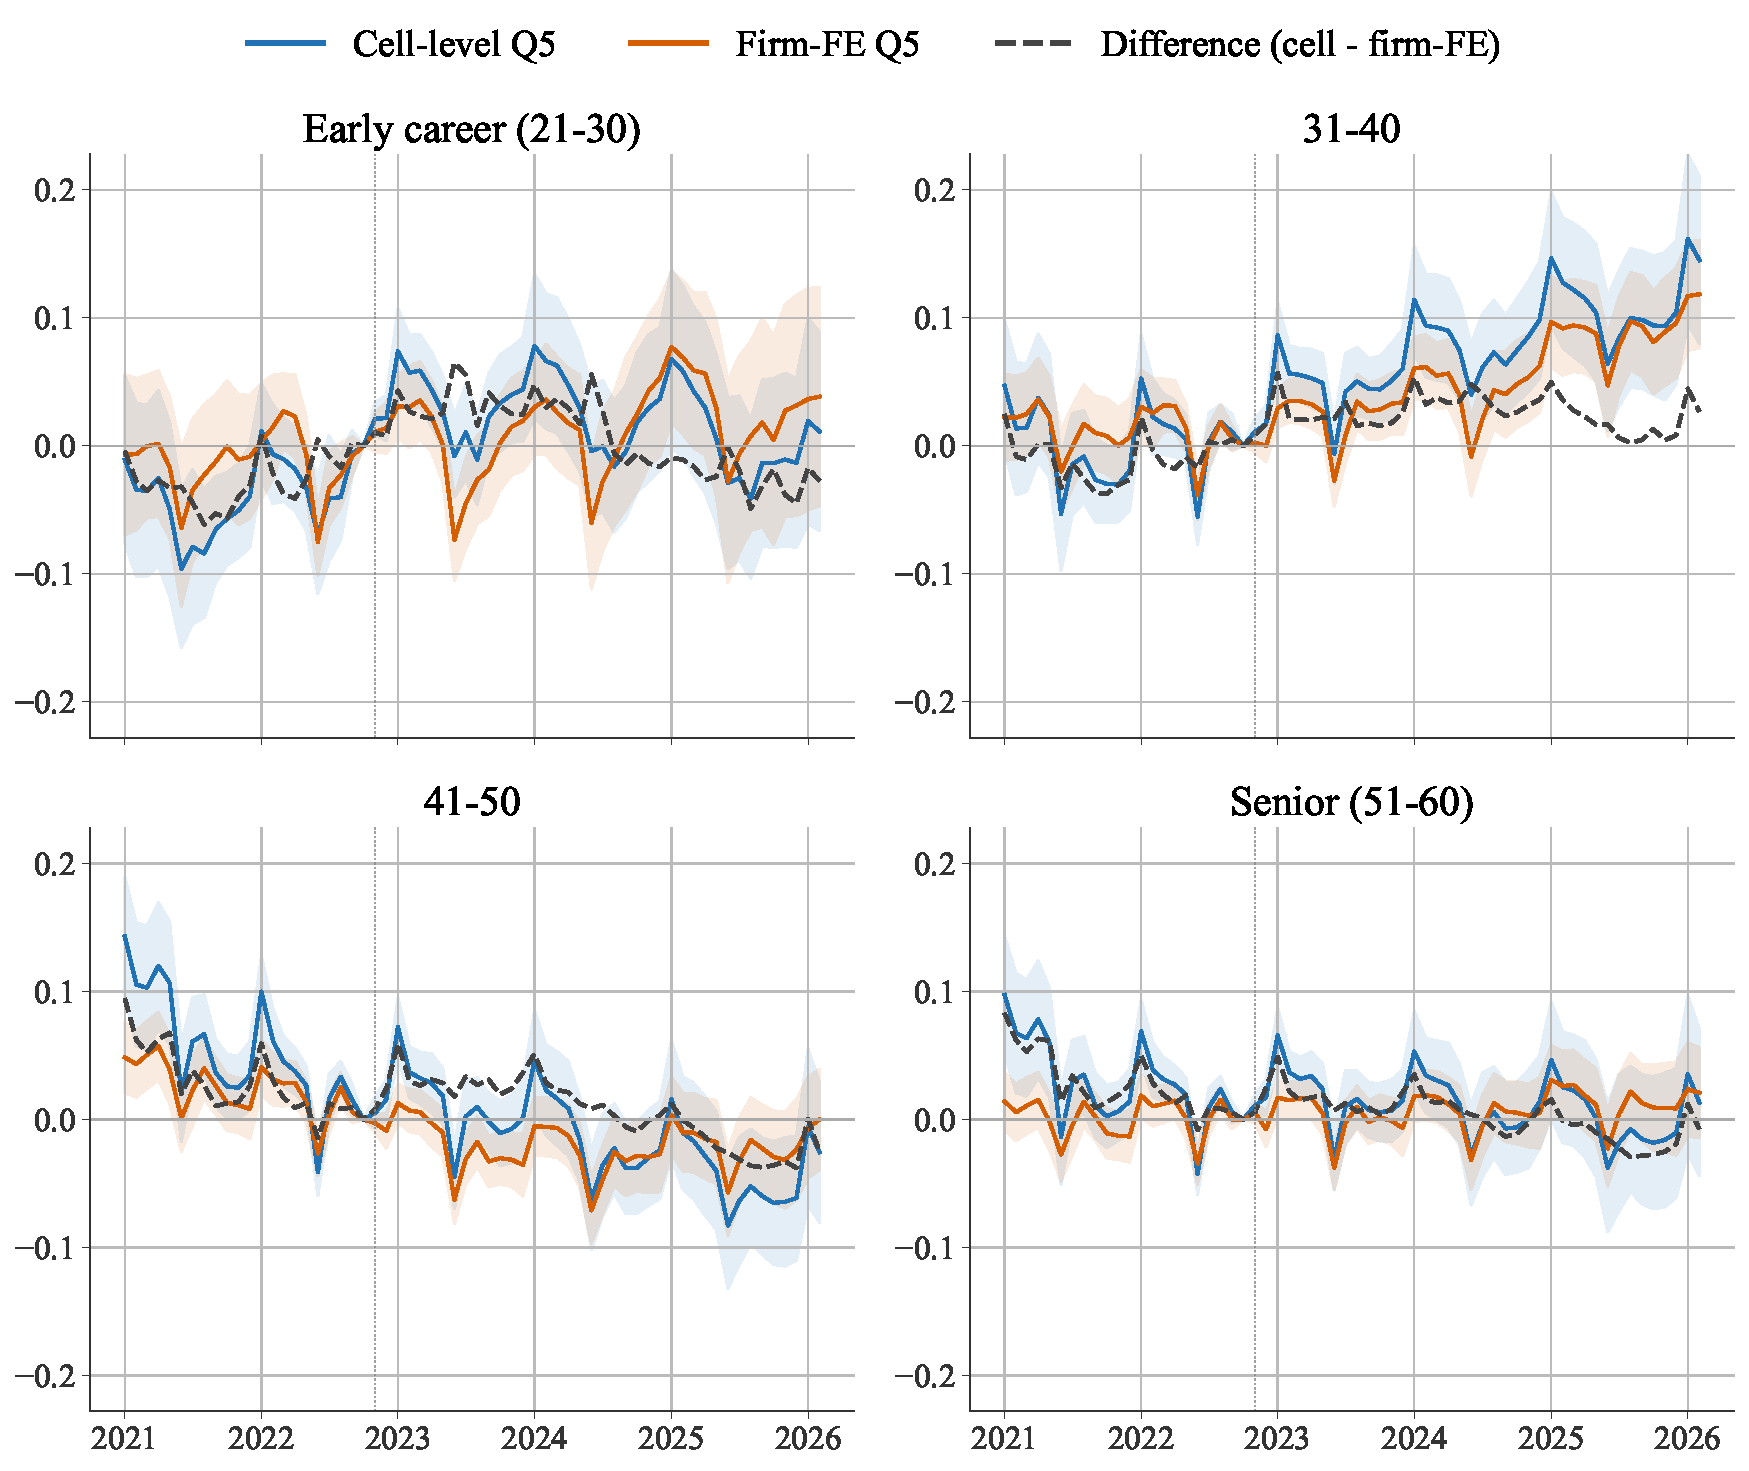
\includegraphics[width=\textwidth]{../analysis/output/figures/figure_cell_vs_firmfe_q5_grid.pdf}
  \caption{Cell-level and firm-FE event-study coefficients for the most-exposed quintile, by decade age group, private sector.}
  \label{fig:cell_vs_firmfe}
  \begin{minipage}{\textwidth}\footnotesize\textit{Notes:} Q5-vs-Q1 Poisson event-study coefficients, in log points, relative to October 2022. Blue: cell-level microdata.no spec (Figure~\ref{fig:microdata_poisson_grid}). Orange: individual-level firm-FE spec (Figure~\ref{fig:firmfe_poisson_grid}). Gray: cell minus firm-FE. Shaded bands: 95\% confidence intervals. Sample 2021m1--2026m2.\end{minipage}
\end{figure}


\subsection{Robust Inference}\label{sec:regression:robust}

Because exposure quintiles were already trending differently before ChatGPT, we treat the event studies as descriptive and use HonestDiD sensitivity to assess how much causal interpretation the data can support. The event studies above display the pre-ChatGPT period, and the pre-period coefficients are not flat. In the cell-level event study the most-exposed quintile's pre-period path moves over a peak-to-trough range of 0.11 to 0.18 log points across the four age groups, as large as or larger than the post-2022 movements, and joint tests reject parallel pre-trends in every age group in both the cell and firm-FE specifications. The pre-period also differs across age groups and across occupations: software developers aged 21--30 are already declining before November 2022 (Figure~\ref{fig:occupations_by_age}), while other occupations are flat.

Two non-AI channels in particular could make the exposure quintiles trend apart for reasons unrelated to AI. The first is a post-COVID technology correction: software, data analysis, and digital services hired aggressively from 2020 through 2022, disproportionately absorbing young workers, and the subsequent correction, as pandemic-era demand for digital services normalized, would reproduce the post-2022 decline in selected occupations with no AI involvement; the 21--30 software developer line in Section~\ref{sec:results} starts to slope down before ChatGPT's release, consistent with this channel. The second is supply-side reallocation: workers entering the labor market after 2022 may be avoiding occupations they perceive as exposed to AI, generating the same young-worker pattern through worker choice rather than employer substitution. The exposure patterns in Figure~\ref{fig:age_by_quintile} are relative, any negative separation being in the most-exposed quintile relative to the least-exposed while the overall age-group line is roughly flat, so the aggregate data alone cannot distinguish occupational reallocation from outright exit. These channels and the AI channel can all be operating at once, and a confound of this kind is exactly what a non-flat pre-trend reflects, which motivates the sensitivity analysis that follows.

These pre-trends bear on interpretation. A difference-in-differences design, including the post-versus-pre estimates in Tables~\ref{tab:did_cell} and~\ref{tab:did_firmfe}, attributes the post-2022 change to the ChatGPT release under the assumption that the most- and least-exposed quintiles would otherwise have moved in parallel. That assumption is debatable here: the quintiles were already on diverging paths before November 2022, and the divergence differs by age group. A collapsed difference-in-differences can therefore read a continuation of a pre-existing trend as an AI effect, and the direction of the resulting bias need not be the same across age groups.

The non-flat pre-period motivates a sensitivity analysis using the honest difference-in-differences approach of \citet{rambachan2023}. This method does not require us to decide whether the parallel-trends assumption is exactly true or false. Instead, it asks how large the post-ChatGPT violation of parallel trends would have to be to overturn the estimated exposure gradient. The method uses the pre-treatment event-study coefficients to discipline the amount of post-treatment confounding that is allowed, and constructs confidence intervals that are valid under the chosen restriction.

We apply the procedure to the Q5-versus-Q1 event-study coefficients from the private-sector Poisson specifications. The main target is the average post-ChatGPT Q5-vs-Q1 employment difference for workers aged 21--30 over the full post period, November 2022 through February 2026, using the same cell-level event study, October 2022 reference, and post window as the difference-in-differences of Section~\ref{sec:regression:age}. The monthly coefficients are aggregated to quarters, so the procedure tests the robustness of exactly that estimate. We also repeat the exercise for the 22--25 Brynjolfsson-style sample of Section~\ref{sec:regression:bcc}, where the Q5--Q1 gap opens only from spring 2025.\footnote{The 22--25 sample uses the exported event-study coefficients and their standard errors; lacking the full variance-covariance matrix of those coefficients, we approximate it as diagonal, which ignores correlation across the event-study coefficients and should be read as indicative.} October 2022 is the last status date before ChatGPT's release on November 30, 2022, so the procedure tests the same event-study path shown in Figure~\ref{fig:microdata_poisson_grid}.

Our preferred sensitivity parameter is the relative-magnitude bound $\bar{M}$. The benchmark value $\bar{M}=1$ allows the post-ChatGPT violation of parallel trends to be as large as the largest violation observed in the pre-ChatGPT period. We also report results for $\bar{M}\in\{0,0.5,1,1.5,2\}$, where $\bar{M}=0$ corresponds to exact parallel trends and $\bar{M}=2$ allows post-period violations twice as large as the worst pre-period violation. We report the breakdown value of $\bar{M}$, the largest value for which the conclusion remains statistically significant.

The sensitivity analysis asks whether the post-2022 exposure gradient survives violations of parallel trends as large as those already visible before ChatGPT. Intervals that include zero for values of $\bar{M}$ near one point to little robustness; one-sided intervals at $\bar{M}\geq 1$ would be stronger evidence.

Table~\ref{tab:honest_did} reports the HonestDiD confidence intervals for the main 21--30 sample. The conventional interval already includes zero, so the robust relative-magnitude intervals include zero at the benchmark $\bar{M}=1$ and at every other value, and the breakdown value is zero. The 21--30 exposure gradient is not a fragile negative estimate; it is essentially absent under the paper's preferred design. For the youngest workers the systematic exposure-quintile result is therefore a precise null: there is no post-ChatGPT employment gradient for the relative-magnitude restriction to overturn, rather than a negative effect whose robustness is in question. This is consistent with the descriptive series, in which the most-exposed quintile does not separate from the least-exposed.

\begin{table}[tp]
  \centering
  \caption{HonestDiD sensitivity of the Q5-vs-Q1 employment effect to violations of parallel trends, ages 21--30, private sector.}
  \label{tab:honest_did}
  \begin{tabular}{lc}
\toprule
Restriction & Robust 95\% CI \\
\midrule
Original ($\bar{M}=0$, parallel trends) & [-0.022, +0.065] \\
$\bar{M}=0.5$ & [-0.221, +0.301] \\
$\bar{M}=1.0$ & [-0.475, +0.555] \\
$\bar{M}=1.5$ & [-0.729, +0.796] \\
$\bar{M}=2.0$ & [-0.983, +1.064] \\
\midrule
Breakdown $\bar{M}$ & 0.00 \\
\bottomrule
\end{tabular}

  \begin{minipage}{\textwidth}\footnotesize\textit{Notes:} Robust 95\% confidence intervals for the average post-ChatGPT Q5-vs-Q1 employment difference (November 2022--February 2026), ages 21--30, private sector, under the relative-magnitude restriction of \citet{rambachan2023}. Monthly event-study coefficients are aggregated to quarters; the target is the average over all post-period quarters, matching the difference-in-differences of Section~\ref{sec:regression:age}. $\bar{M}=0$ imposes exact parallel trends; $\bar{M}=1$ allows post-period violations as large as the worst pre-period violation. ``Breakdown'' is the largest $\bar{M}$ for which the interval excludes zero. ``Original'' is the conventional 95\% interval. Computed from the cell-level Poisson event study of Section~\ref{sec:regression:age}.\end{minipage}
\end{table}


% =============================================================================

\subsection{Replication of the design of Brynjolfsson et al.\ (2025)}\label{sec:regression:bcc}

In the main analyses, we use decade age groups, 21--30 and so on. To ease comparison with the cross-country literature that uses a narrower 22--25 early-career definition, we replicate the \citet{brynjolfsson2025} design using that definition. The sample is a balanced panel of full-time private-sector workers in firms, with workers placed in six age bins from 22--25 to 50--55 and occupations ranked by the Eloundou GPT-4 quintile; the construction and supporting figures are in Appendix~\ref{app:bcc}.

For workers aged 22--25 the post-October-2022 average Q5-vs-Q1 gap is small, about 3 log points, but it masks a clear time profile (Appendix Figure~\ref{fig:bcc_es}): the most- and least-exposed quintiles track each other through early 2025, and from spring 2025 the most-exposed quintile falls below, with the gap widening to about 35 log points by February 2026. The recent gap exceeds the 15 log points \citet{brynjolfsson2025} report for the United States.

% =============================================================================
\section{Discussion}\label{sec:discussion}

\subsection{Cross-Country Comparison}\label{sec:discussion:crosscountry}

Table~\ref{tab:crosscountry} summarizes the cross-country evidence, separating descriptive time series (Panel~A) from formal econometric estimates (Panel~B).

On the descriptive case studies, Norway looks like the US and Sweden. Every country with a descriptive analysis shows an early-career decline in AI-exposed occupations except Finland, and the Norwegian per-capita decline of about 18 percent for young software developers sits between the US ($-20\%$, \citealp{brynjolfsson2025}) and the Swedish raw figure ($-44\%$, \citealp{lodefalk2026}). On the systematic full-distribution evidence, Norway looks like Denmark and Finland: ranking all occupations by exposure, the most-exposed quintile does not decline among young workers, and the narrow 22--25 replication diverges only late and on rejected pre-trends (Section~\ref{sec:regression:bcc}).

It does not rule out an AI role: formal designs may absorb effects that operate outside direct firm-level adoption, such as competitive pressure from AI-adopting rivals or supply-side reallocation by workers anticipating disruption. But it does make the descriptive trends, including ours, hard to interpret on their own, because monetary tightening and the post-COVID correction may move the same occupations. \citet{humlum2026}, the only study with individual-level adoption data, finds that workplace AI-chatbot adoption does not drive the Danish early-career decline; \citet{lodefalk2026} attribute much of the Swedish decline to the Riksbank rate cycle; and at the industry level \citet{bick2026} find no clear link between AI adoption and employment in either Europe or the US. Norway, Sweden, Denmark, and Finland share similar institutions yet differ in their formal results, so institutional structure alone does not explain the heterogeneity.

\begin{table}[htbp]
\centering
\caption{Cross-Country Comparison of Early Labor Market Patterns under Generative AI}
\label{tab:crosscountry}
\footnotesize
\newcolumntype{Y}{>{\hsize=1.8\hsize\raggedright\arraybackslash}X}
\newcolumntype{Z}{>{\hsize=0.65\hsize\raggedright\arraybackslash}X}
\begin{tabularx}{\textwidth}{@{}Z Z Z Z Y@{}}
\toprule
Country & Study & Method & Direction (22--25) & Notes \\
\midrule
\multicolumn{5}{@{}l}{\textit{Panel A: Descriptive time series}} \\[2pt]
US & Brynjolfsson et al.\ (2025) & Descriptive & Decline & SW developers 22--25: $-20\%$; top-2 quintiles: $-6\%$ \\[4pt]
Sweden & Lodefalk et al.\ (2026) & Descriptive & Decline & $\approx -44\%$ raw in top quartile (Fig.\ A23) \\[4pt]
Denmark & Humlum \& Vestergaard (2026) & Descriptive & Decline & Aggregate early-career decline mirrors US (App.\ D.2) \\[4pt]
Finland & Kauhanen \& Rouvinen (2026) & Descriptive & Null & Trends reflect demographics, not AI \\[4pt]
UK & Teeselink (2025) & Descriptive & Decline & High-wage, junior positions \\[4pt]
Norway & This paper & Descriptive & Decline (selected occupations) & Software developers 21--30: $-18\%$ (Fig.~\ref{fig:occupations_by_age}); no Q5--Q1 divergence at 21--30 (Fig.~\ref{fig:age_by_quintile}) \\[6pt]
\multicolumn{5}{@{}l}{\textit{Panel B: Formal estimation}} \\[2pt]
US & Brynjolfsson et al.\ (2025) & Poisson event study, firm FE & Decline & $-15$ log pts, most vs.\ least exposed quintile \\[4pt]
Sweden & Lodefalk et al.\ (2026) & DiD, employer FE & Decline & $-5.5\%$ within-employer by 2025H1; posting decline driven by rate hikes, not AI \\[4pt]
Denmark & Humlum \& Vestergaard (2026) & DiD, worker/workplace FE & Null & Aggregate decline not driven by firm AI adoption; rules out $>2\%$ earnings effect \\[4pt]
UK & Teeselink (2025) & DiD & Decline & Junior positions at high-wage firms \\[4pt]
Norway & This paper & Poisson event study, firm FE & Mixed / late decline & 22--25: near zero on average, Q5 falls below Q1 from spring 2025 to $\approx -35$ log pts by early 2026; 21--30 $\approx 0$ (App.\ B) \\
\bottomrule
\end{tabularx}
\par\smallskip\footnotesize
\raggedright\textit{Notes:} Studies sorted by year within each panel. ``Direction'' refers to the qualitative sign of the relative employment change for workers aged 22--25 in the most AI-exposed occupations after November 2022. Panel~A reports descriptive patterns (raw or per-capita trends); Panel~B reports results from formal econometric methods with controls and fixed effects. The descriptive-formal gap is substantial in all studies that employ both: Lodefalk et al.\ find $-44\%$ raw vs.\ $-5.5\%$ in the employer-FE event study; Humlum \& Vestergaard find an aggregate decline descriptively but a precise null when using firm-level adoption as treatment. Norway shows a descriptive young-worker decline in selected occupations and a 22--25 formal estimate that is near zero on average but widens to a sizable gap at the end of the sample (App.\ B replicates the Brynjolfsson et al.\ design on Norwegian data). Magnitudes across rows use different units and baselines and are not directly comparable.
\end{table}


A limited wage response is consistent with Norway's two-tier bargaining system \citep{bhuller2022} channelling any AI-related adjustment toward the quantity margin in the private sector. Downward-rigid wage floors limit short-run wage adjustment; the locally negotiated drift channel could deliver a wage response over a longer horizon. 

\subsection{The Companion Dashboard}\label{sec:discussion:dashboard}

The public dashboard at kiindeksen.no/en publishes the monthly series used in the paper by age group and AI-exposure quintile \citep{kiindeksen2026}. It updates as new register months arrive and lets readers change the indexing, seasonal adjustment, and smoothing. The paper documents the definitions, sample restrictions, and regression checks behind the dashboard. The purpose of the dashboard is to monitor developments in as live a fashion as possible.

The dashboard headline, the ``KI-indeks,'' is the relative employment growth of the most- versus least-exposed quintile over the most recent three months relative to October 2022, pooled over private-sector workers aged 21 to 60 and seasonally adjusted; it is a descriptive growth gap, not a regression coefficient. Because the seasonal factors are estimated once over 2021 to 2024 and held fixed, the only input that changes as data accrue is which three months form the most recent window. The published value in the most recent vintage, which contains data up to and including February 2026, is a relative growth of about $-0.2$ percentage points. Re-estimating it on expanding windows, one month at a time from data through January 2025 to February 2026, the headline drifts from about $+1.7$ to about $-0.2$ percentage points (Appendix Figure~\ref{fig:recursive_kiindeks}). An occupation cluster bootstrap puts the standard error at roughly two percentage points throughout, so the index is never statistically distinguishable from zero in any vintage, and the full drift over 2025 is comparable to a single vintage's bootstrap standard error. For a live indicator this sets what to watch for. In every vintage so far the index is consistent with zero, so the most-exposed quintile shows no detectable separation from the least-exposed. The month-to-month movements, including the recent dip below zero, stay inside the bootstrap band and are noise; a genuine change would show up only as a sustained move beyond it. 

% =============================================================================
\section{Conclusion}\label{sec:conclusion}
\label{sec:conclusion}

We use monthly population registers to test whether the canary pattern generalizes beyond selected occupations, and it largely does not. Among the youngest workers, whose employment renews through entry and is least confounded by demographic change, selected high-exposure occupations show falling employment, but the systematic exposure ranking does not: the most-exposed quintile does not separate from the least-exposed for workers aged 21 to 30, and new hires and cash earnings show no comparable gradient. The one systematic gap, in the narrow 22--25 sample, opens only from spring 2025 and widens by early 2026.

We do not identify what drives the selected-occupation pattern. Pre-ChatGPT trends differ across age and occupation groups, so a difference-in-differences design that assumes parallel trends can mislead here. AI-related adjustment, the post-COVID correction in technology hiring, monetary tightening, and supply-side reallocation could each generate the same age--exposure gradient, and the aggregate data cannot tell them apart. New data will show whether the recent occupation-specific patterns persist. That is why the dashboard for early AI labor-market monitoring based on the full population is part of the empirical contribution. 


% =============================================================================
% References
% =============================================================================

\clearpage
\bibliography{references}


% =============================================================================
% Appendix
% =============================================================================

\clearpage
\appendix
\phantomsection
\addcontentsline{toc}{section}{Appendix A: Additional Figures}
\section*{Appendix A: Additional Figures}
\setcounter{figure}{0}
\renewcommand{\thefigure}{A\arabic{figure}}
\setcounter{table}{0}
\renewcommand{\thetable}{A\arabic{table}}

\begin{figure}[htbp]
  \centering
  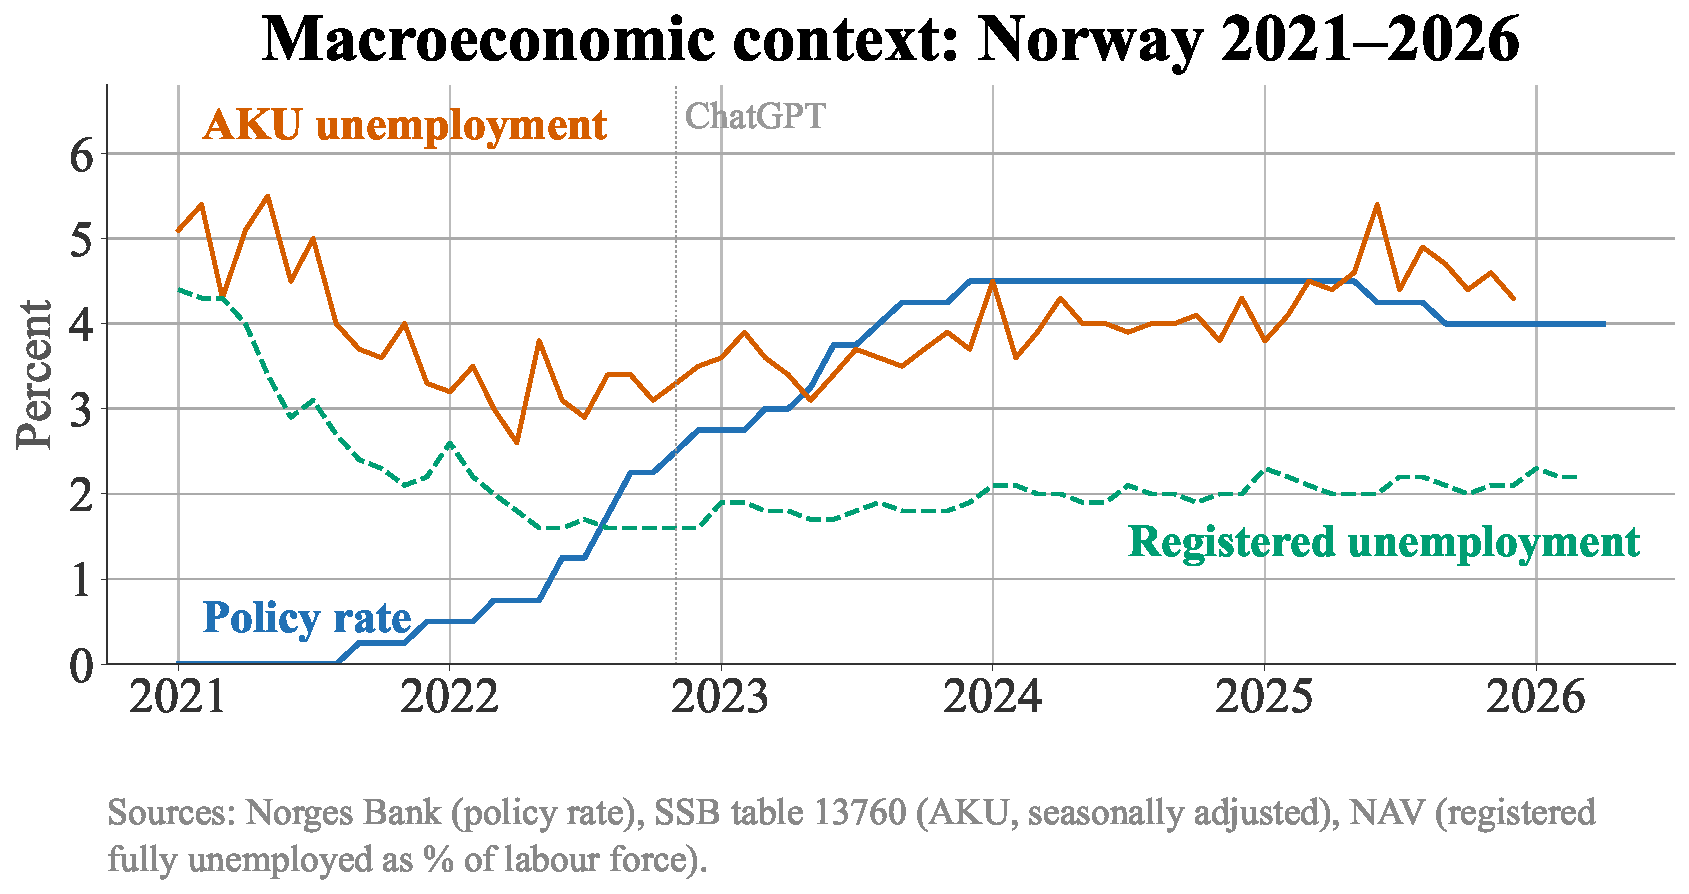
\includegraphics[width=0.8\textwidth]{../analysis/output/figures/figureA0a_macro_context.pdf}
  \caption{Macroeconomic context: Norges Bank policy rate and registered unemployment rate, 2021--2026.}
  \label{fig:macro_context}
\end{figure}

\begin{figure}[htbp]
  \centering
  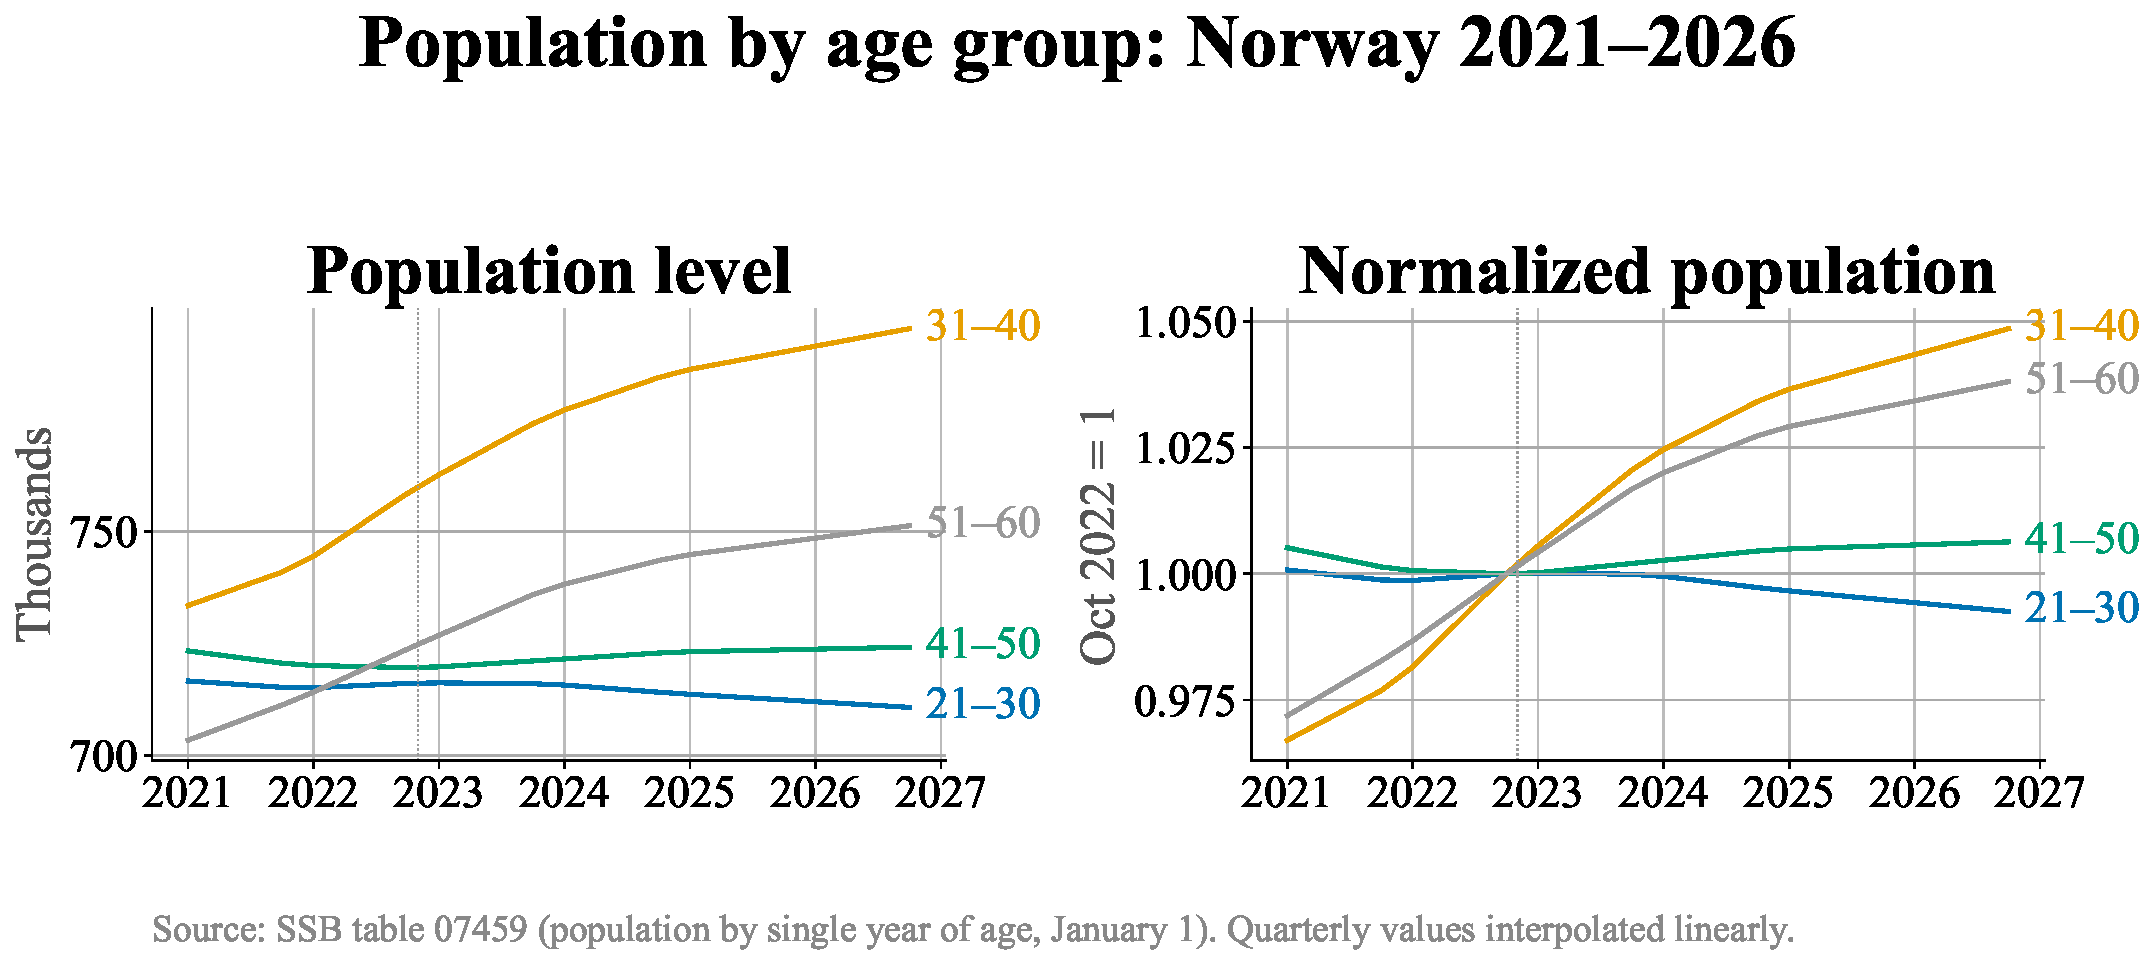
\includegraphics[width=0.8\textwidth]{../analysis/output/figures/figureA0b_cohort_sizes.pdf}
  \caption{Resident population by decade age group, 2021--2026.}
  \label{fig:cohort_sizes}
\end{figure}

% Raw (unadjusted) twins of the main-text descriptive figures
\begin{figure}[htbp]
  \centering
  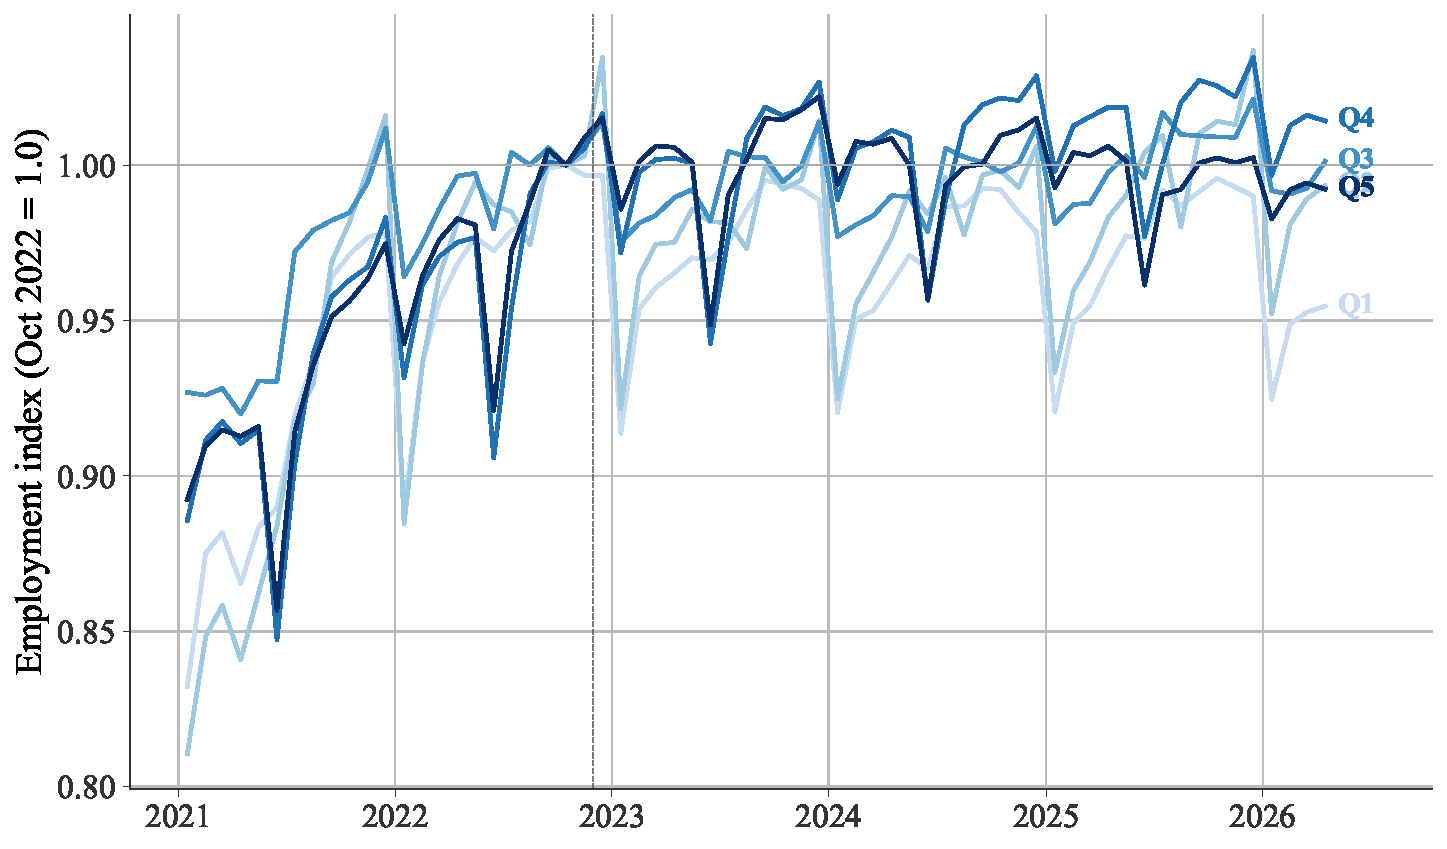
\includegraphics[width=0.85\textwidth]{../analysis/output/figures/figure_emp_byexposure.pdf}
  \caption{Employment by AI-exposure quintile, all ages 21--60, private sector, raw (unadjusted).}
  \label{fig:byexposure_raw}
  \begin{minipage}{\textwidth}\footnotesize\textit{Notes:} Raw (not seasonally adjusted) twin of Figure~\ref{fig:byexposure_sa}; private-sector headcount pooled over ages 21--60, indexed to October 2022 = 1. Occupations are ranked by the Eloundou et al.\ GPT-4 score. The same series, with user-adjustable smoothing, is on the companion dashboard \citep{kiindeksen2026}.\end{minipage}
\end{figure}

\begin{figure}[htbp]
  \centering
  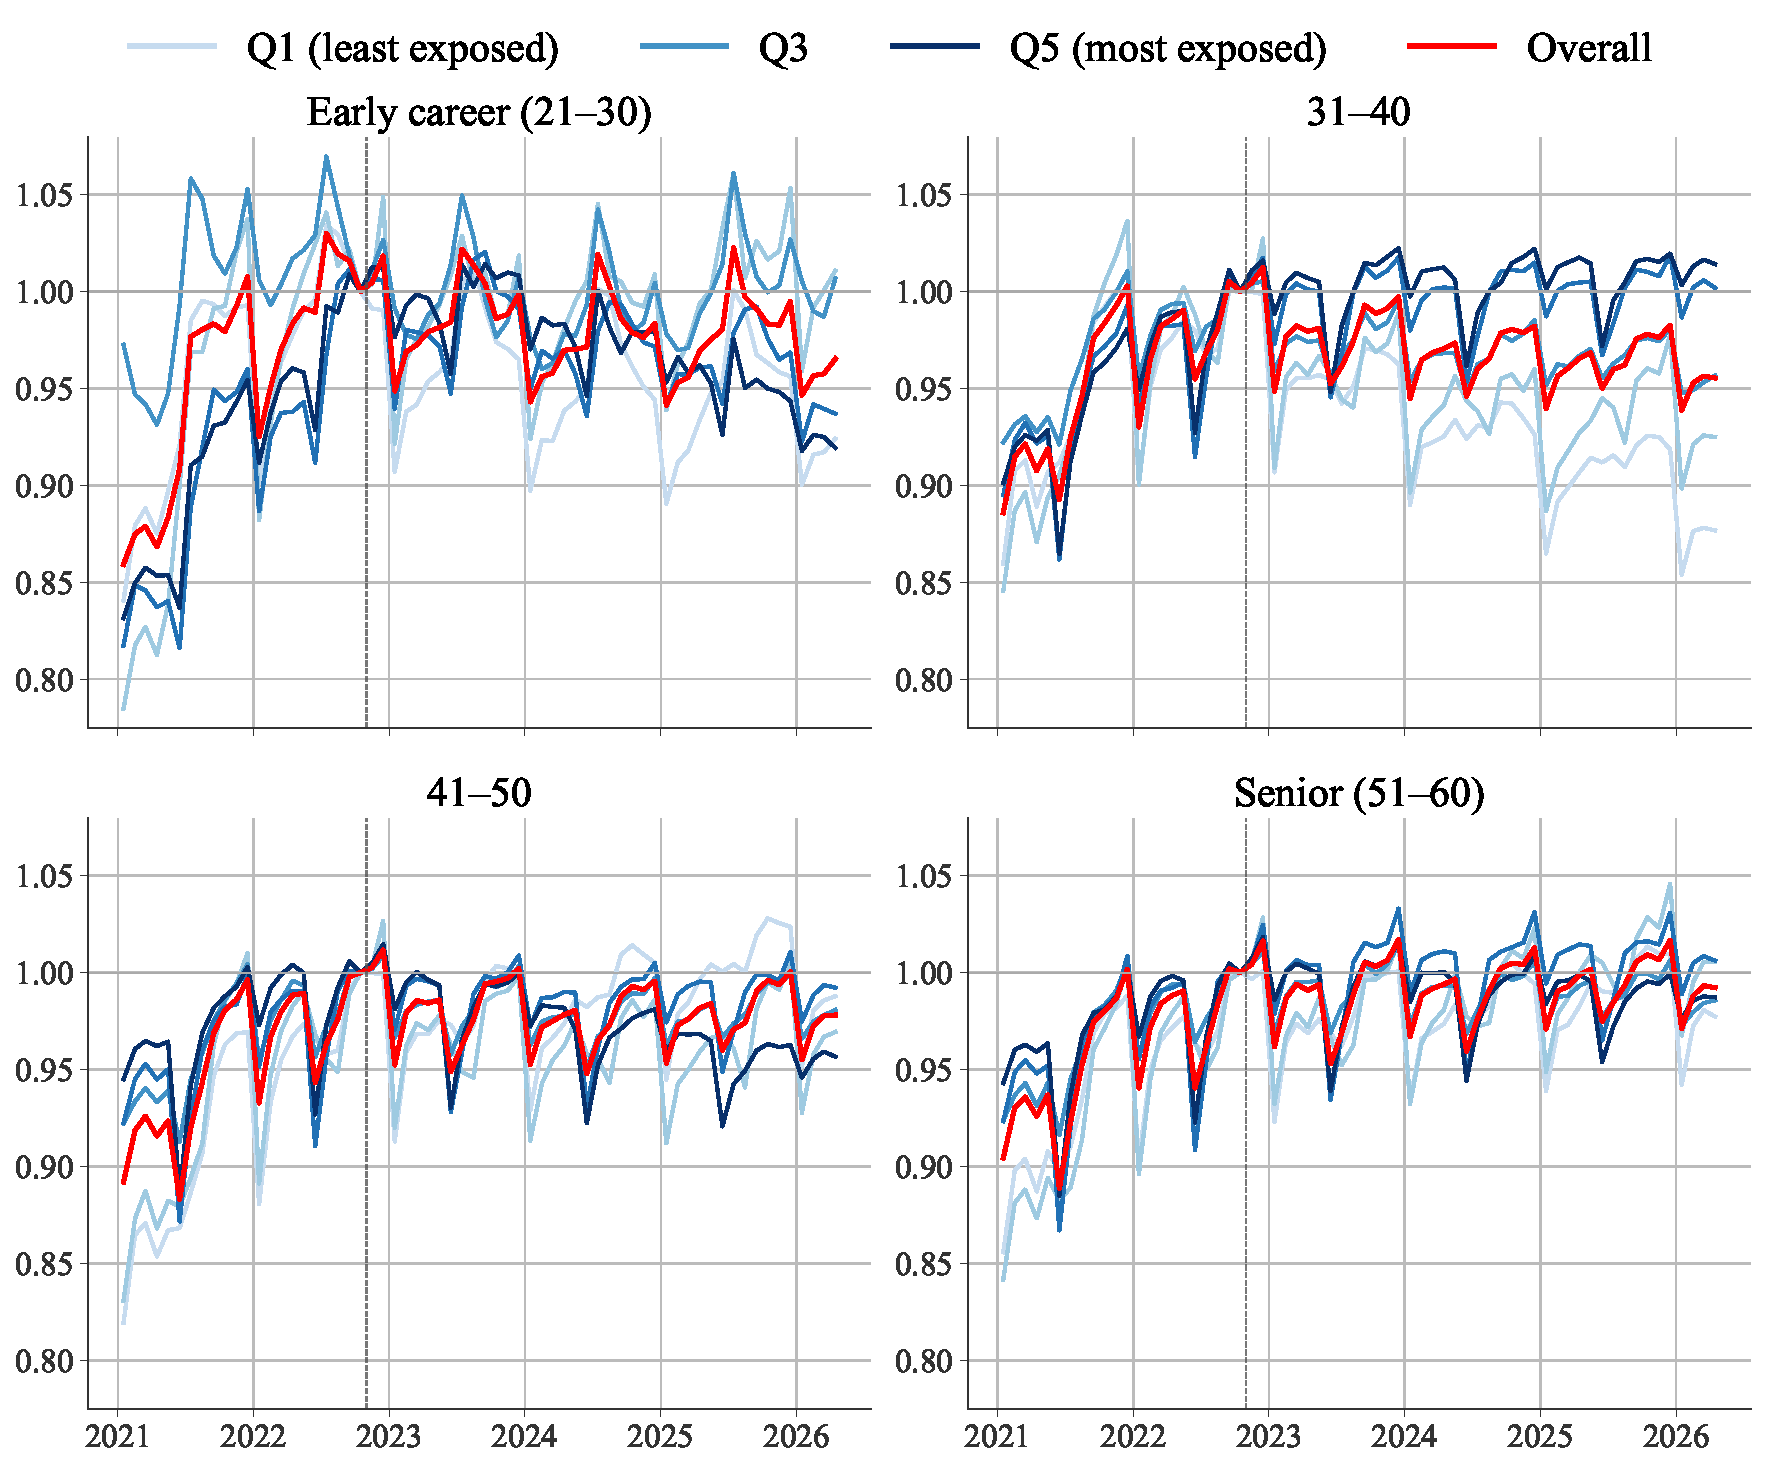
\includegraphics[width=\textwidth]{../analysis/output/figures/figure_emp_decade_private.pdf}
  \caption{Employment by AI-exposure quintile and decade age group, private sector, raw (unadjusted).}
  \label{fig:age_by_quintile_raw}
  \begin{minipage}{\textwidth}\footnotesize\textit{Notes:} Raw (not seasonally adjusted) twin of Figure~\ref{fig:age_by_quintile}; private-sector employment per capita, indexed to October 2022 = 1. Occupations are ranked by the Eloundou et al.\ GPT-4 score. Q1 (lightest) = least exposed; Q5 (darkest) = most exposed. The same series, with user-adjustable smoothing, is on the companion dashboard \citep{kiindeksen2026}.\end{minipage}
\end{figure}

\begin{figure}[htbp]
  \centering
  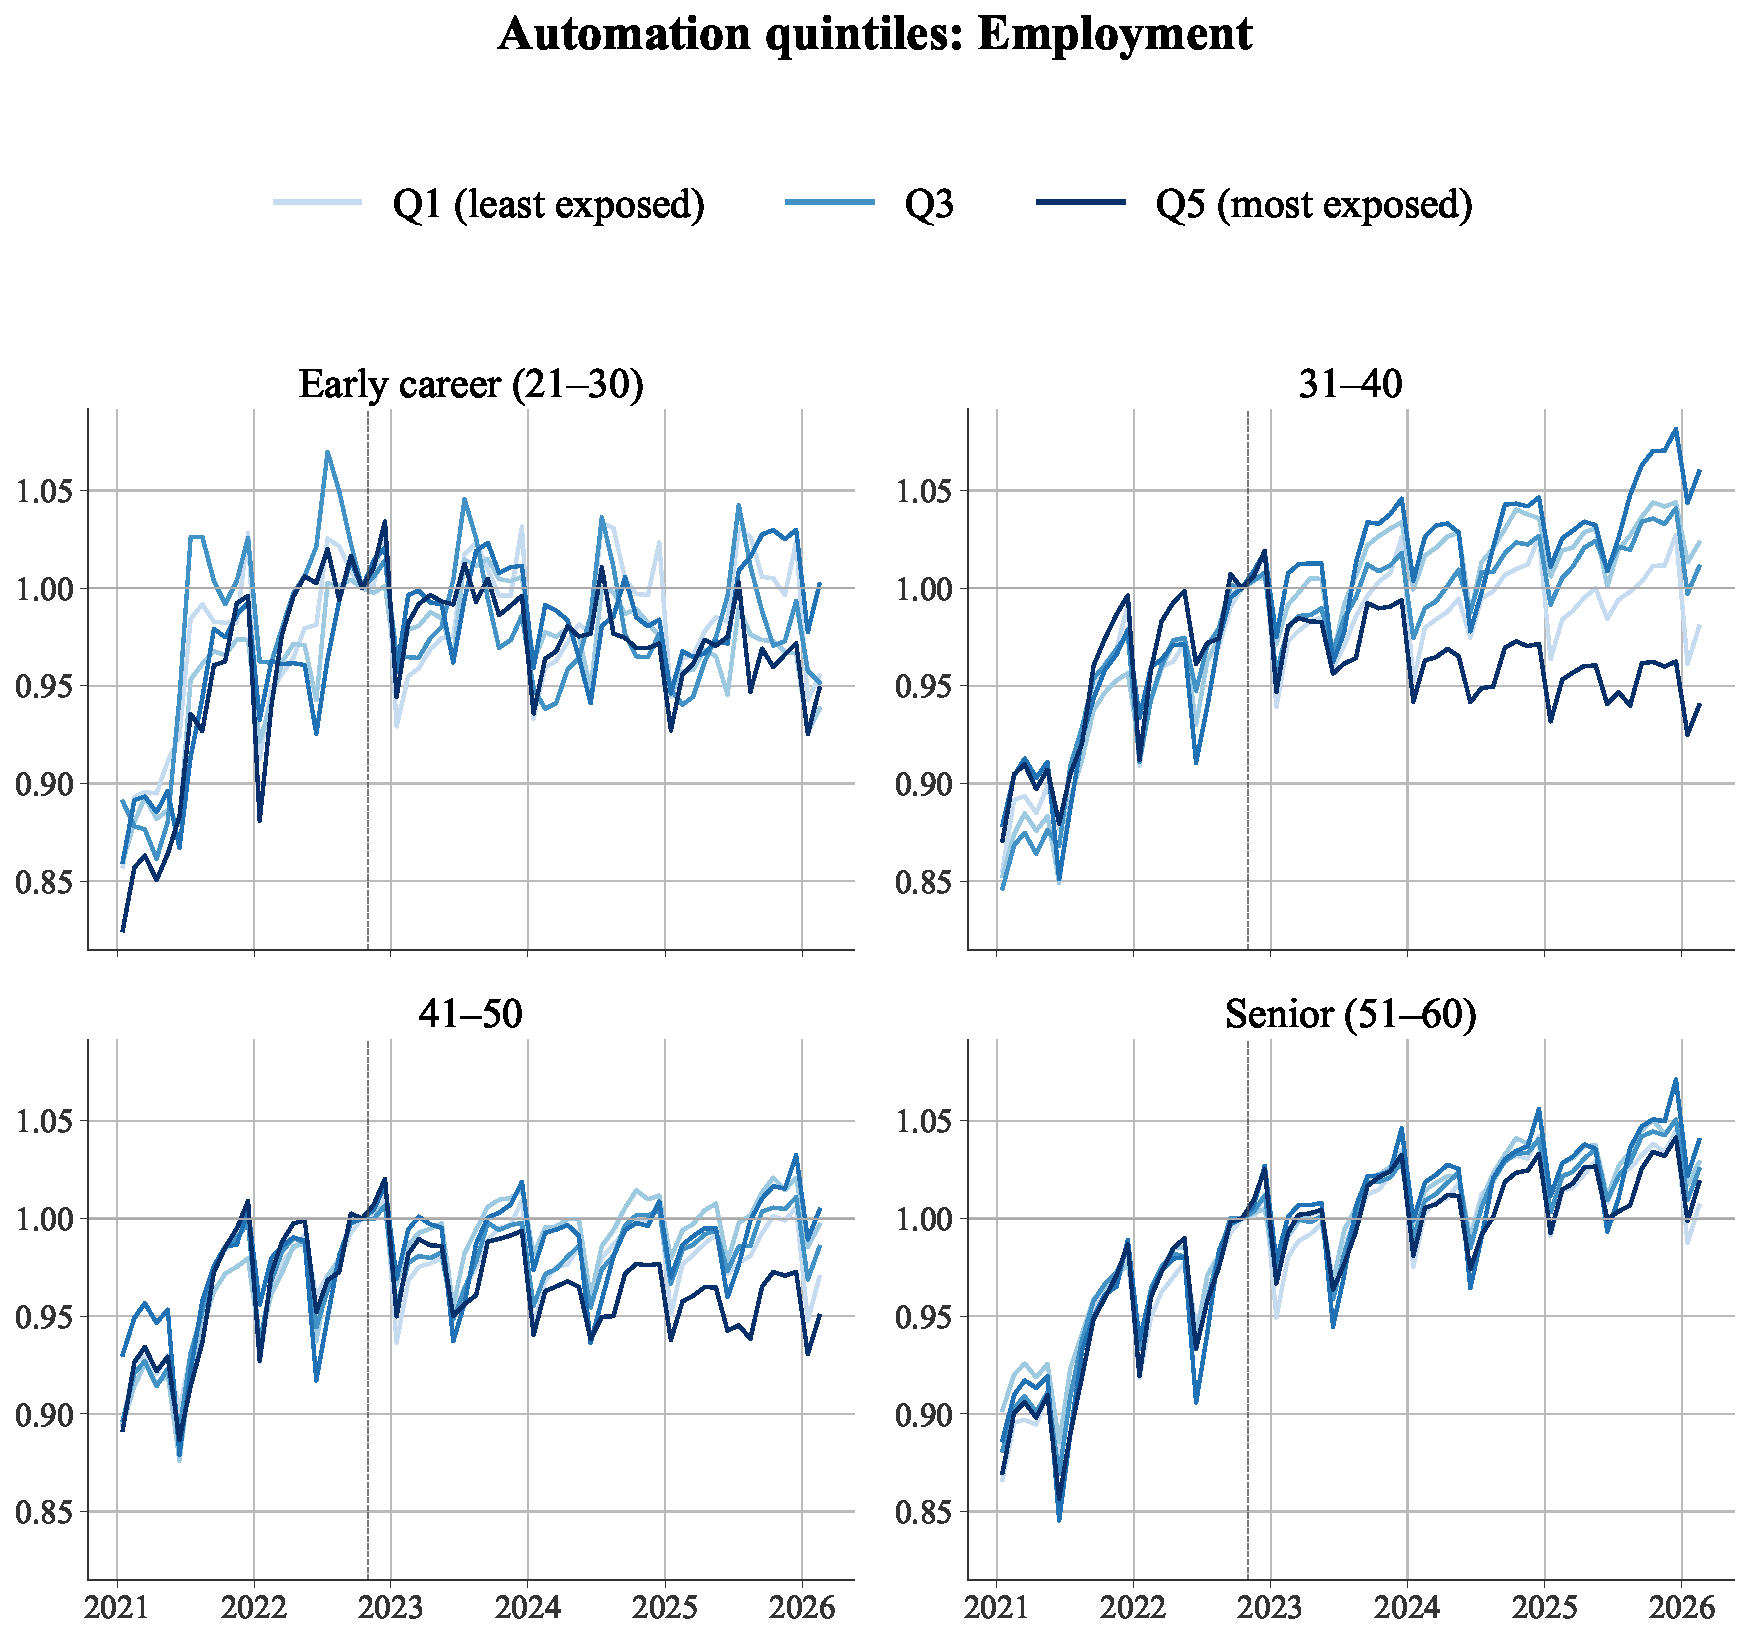
\includegraphics[width=\textwidth]{../analysis/output/figures/figure5b_age_by_quintile_handa.pdf}
  \caption{Employment by Handa et al.\ automation-exposure quintile and decade age group, private sector.}
  \label{fig:age_by_quintile_handa_auto}
  \begin{minipage}{\textwidth}\footnotesize\textit{Notes:} Private-sector employment indexed to October 2022 = 1. Occupations are ranked by the Handa et al.\ automation share.\end{minipage}
\end{figure}

\begin{figure}[htbp]
  \centering
  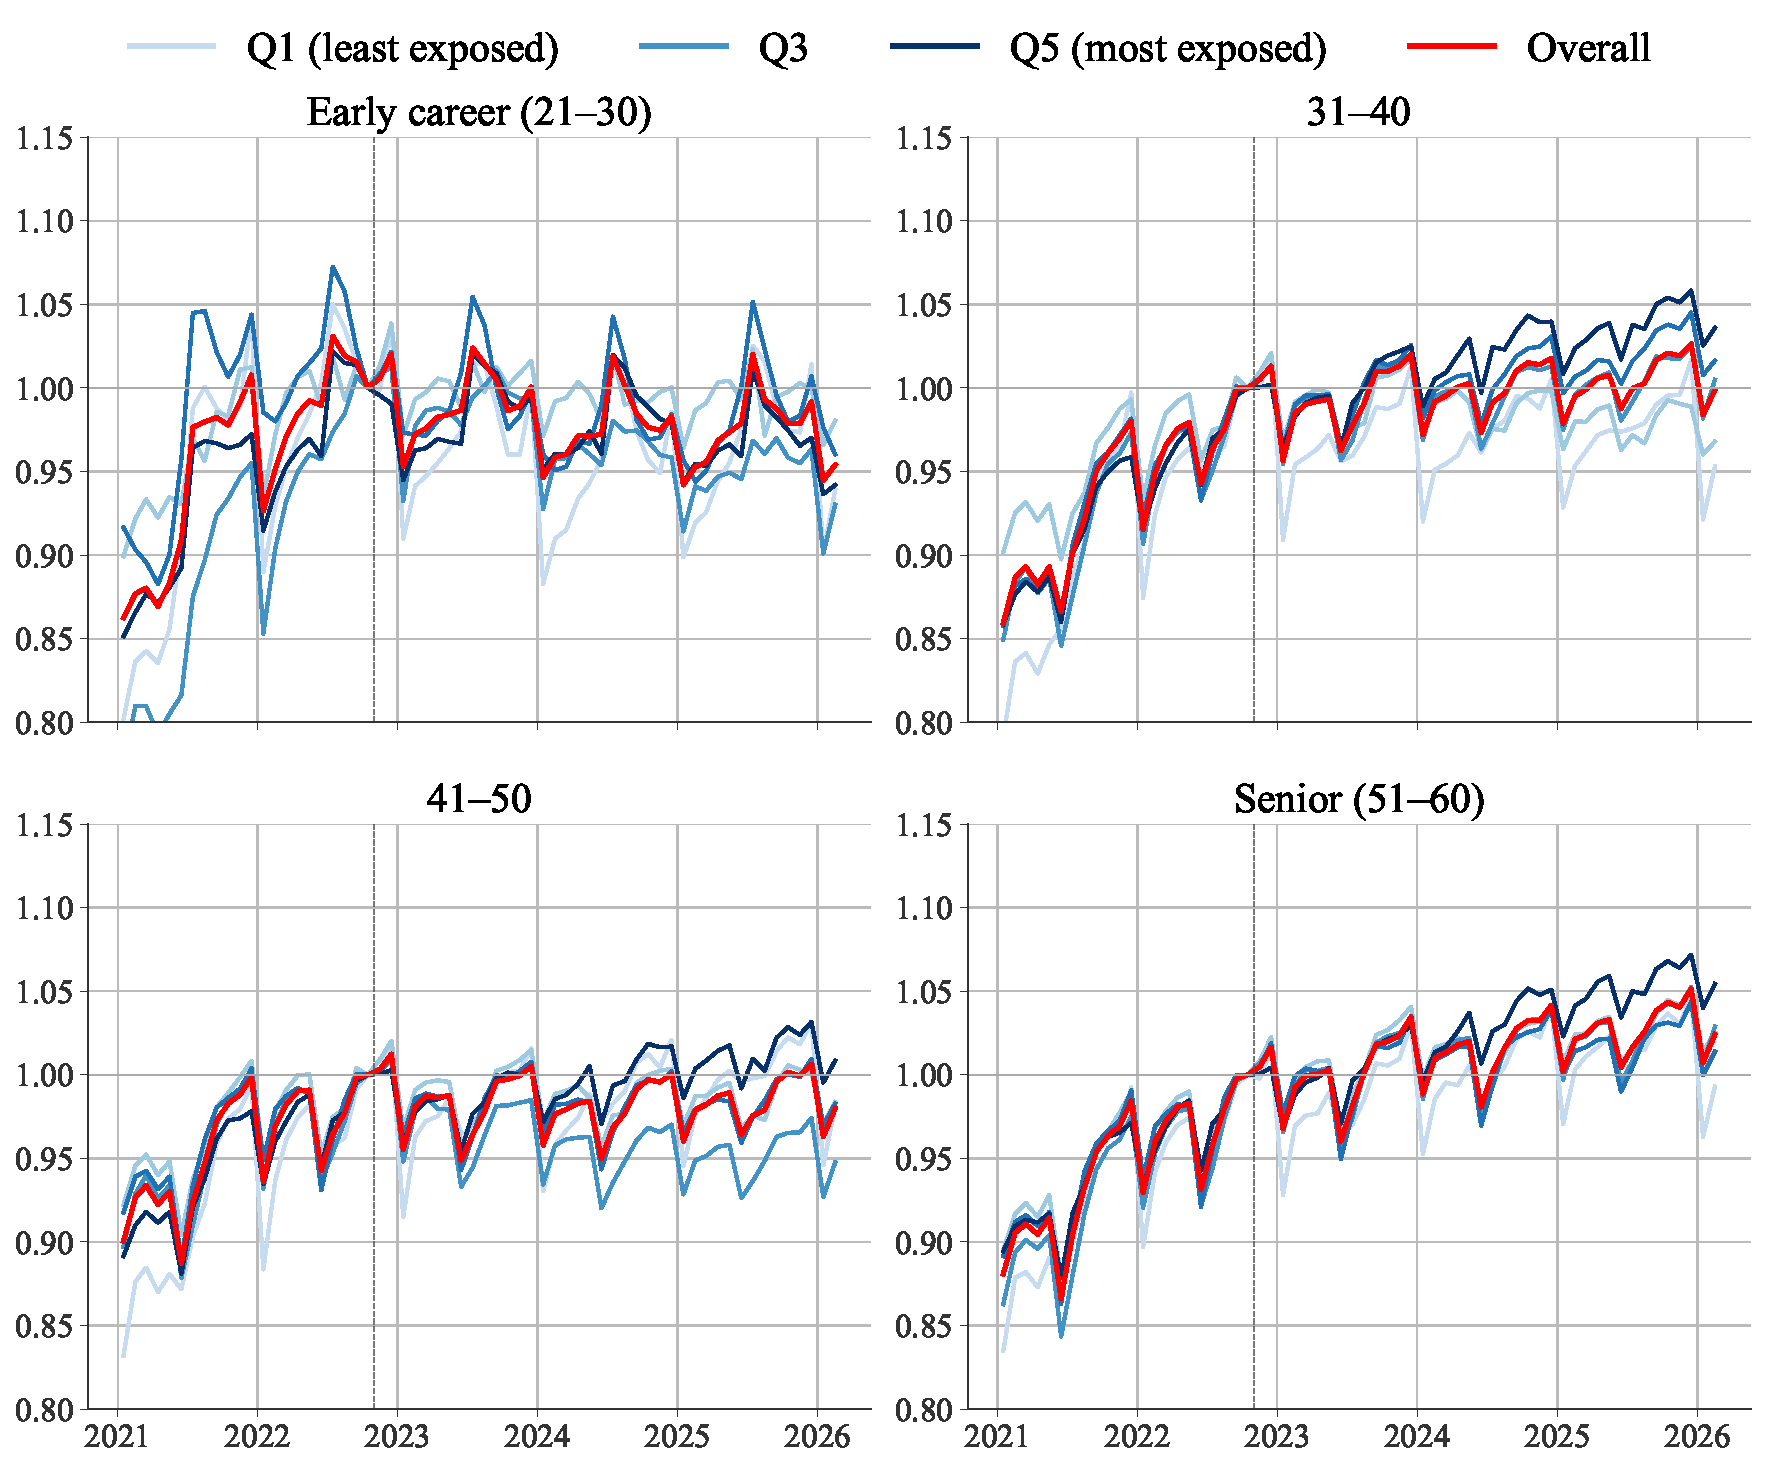
\includegraphics[width=\textwidth]{../analysis/output/figures/figure5c_age_by_quintile_handa.pdf}
  \caption{Employment by Handa et al.\ augmentation-exposure quintile and decade age group, private sector.}
  \label{fig:age_by_quintile_handa_aug}
  \begin{minipage}{\textwidth}\footnotesize\textit{Notes:} Private-sector employment indexed to October 2022 = 1. Occupations are ranked by the Handa et al.\ augmentation share.\end{minipage}
\end{figure}

\begin{figure}[htbp]
  \centering
  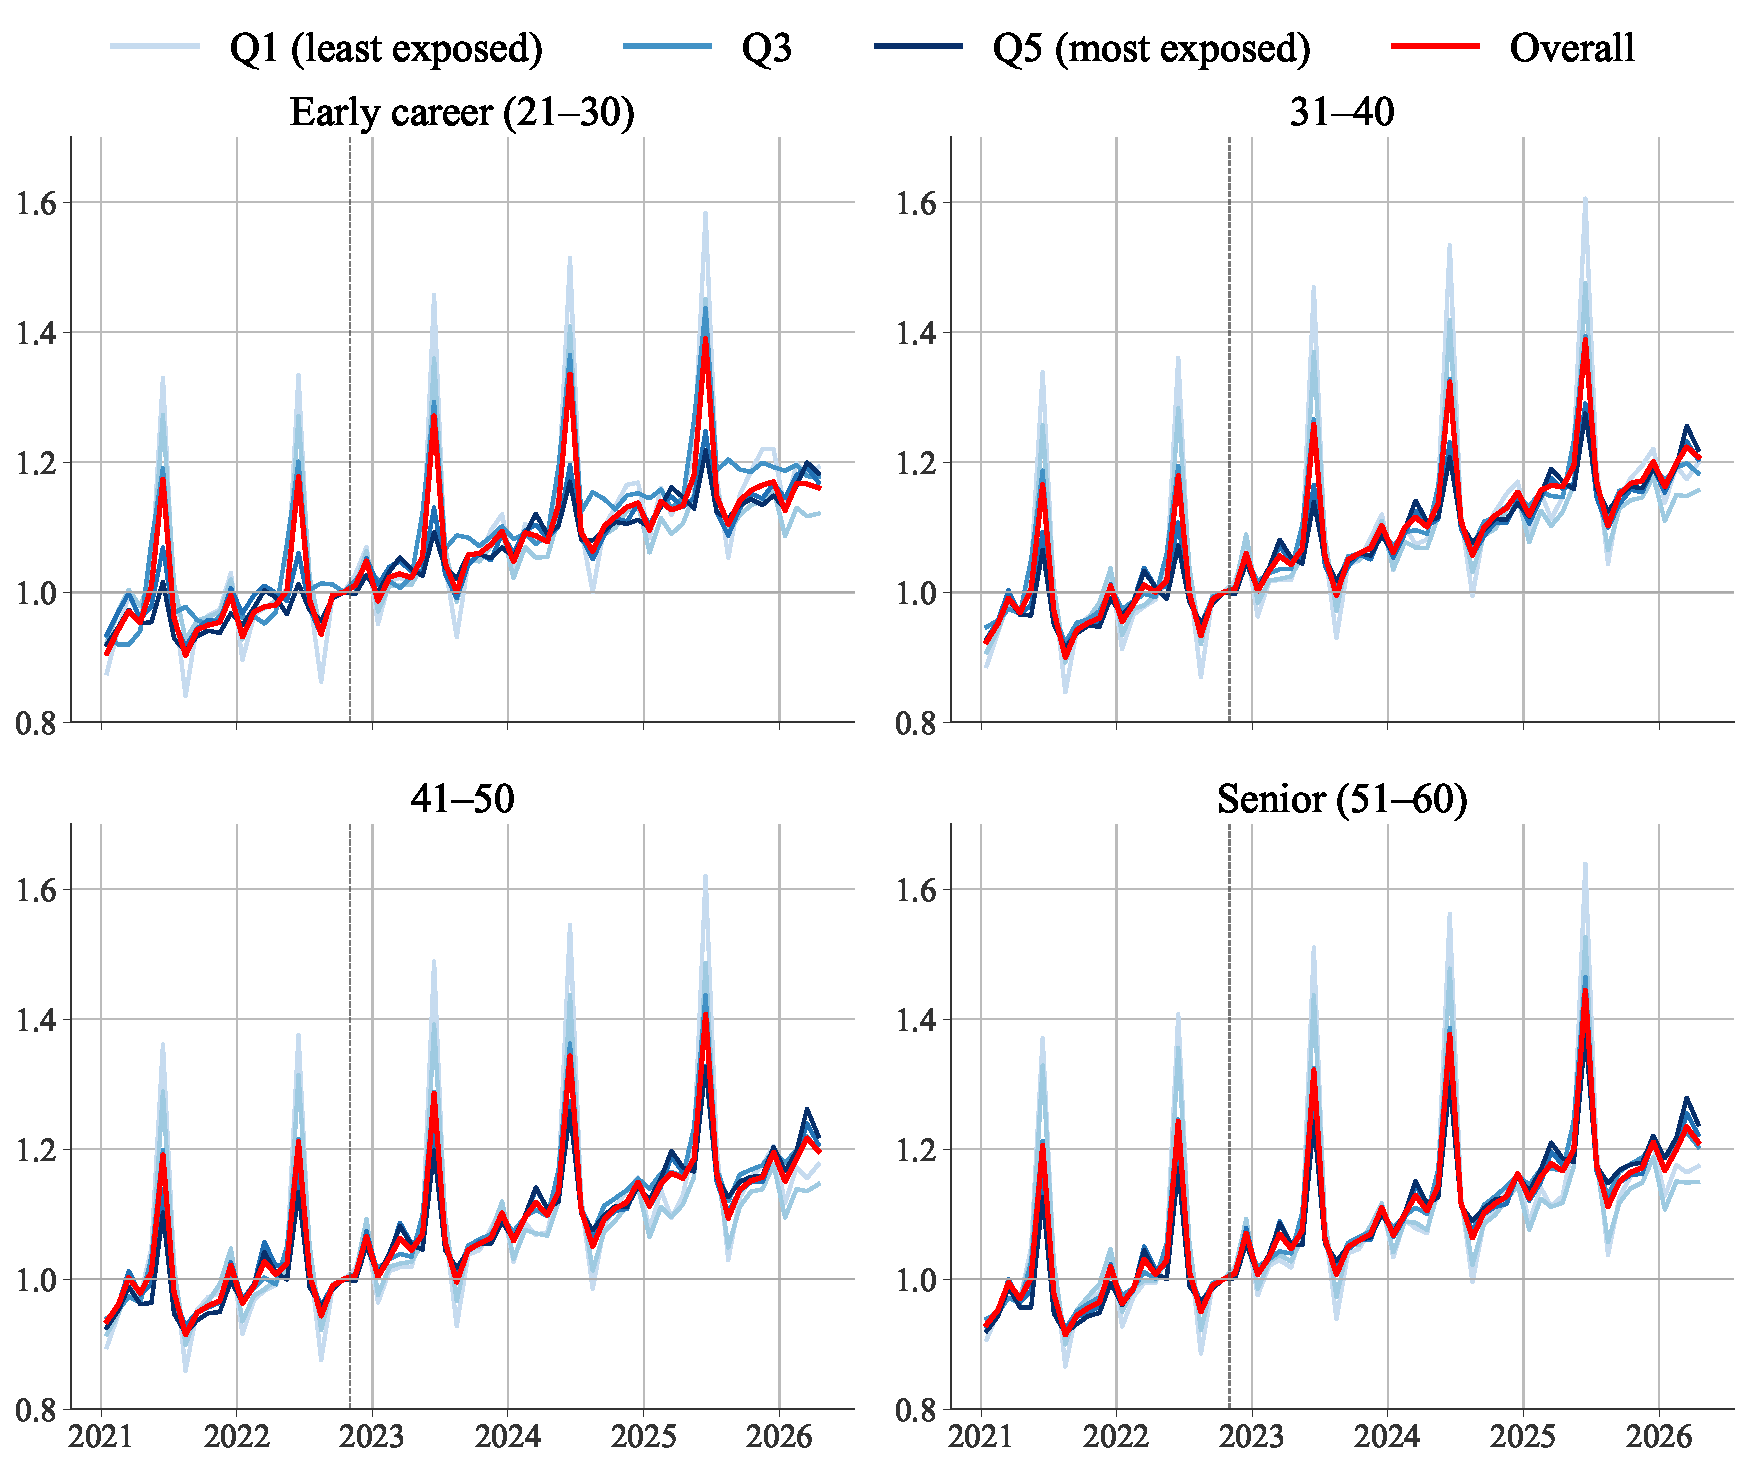
\includegraphics[width=\textwidth]{../analysis/output/figures/figure_kontantlonn_decade_private.pdf}
  \caption{Monthly cash earnings by AI-exposure quintile and decade age group, private sector.}
  \label{fig:kontantlonn_by_quintile}
  \begin{minipage}{\textwidth}\footnotesize\textit{Notes:} Mean monthly cash earnings, indexed to October 2022 = 1. Occupations are ranked by the Eloundou et al.\ exposure score. Strong seasonal patterns (December bonuses, June holiday pay) are visible in all panels.\end{minipage}
\end{figure}

\begin{figure}[htbp]
  \centering
  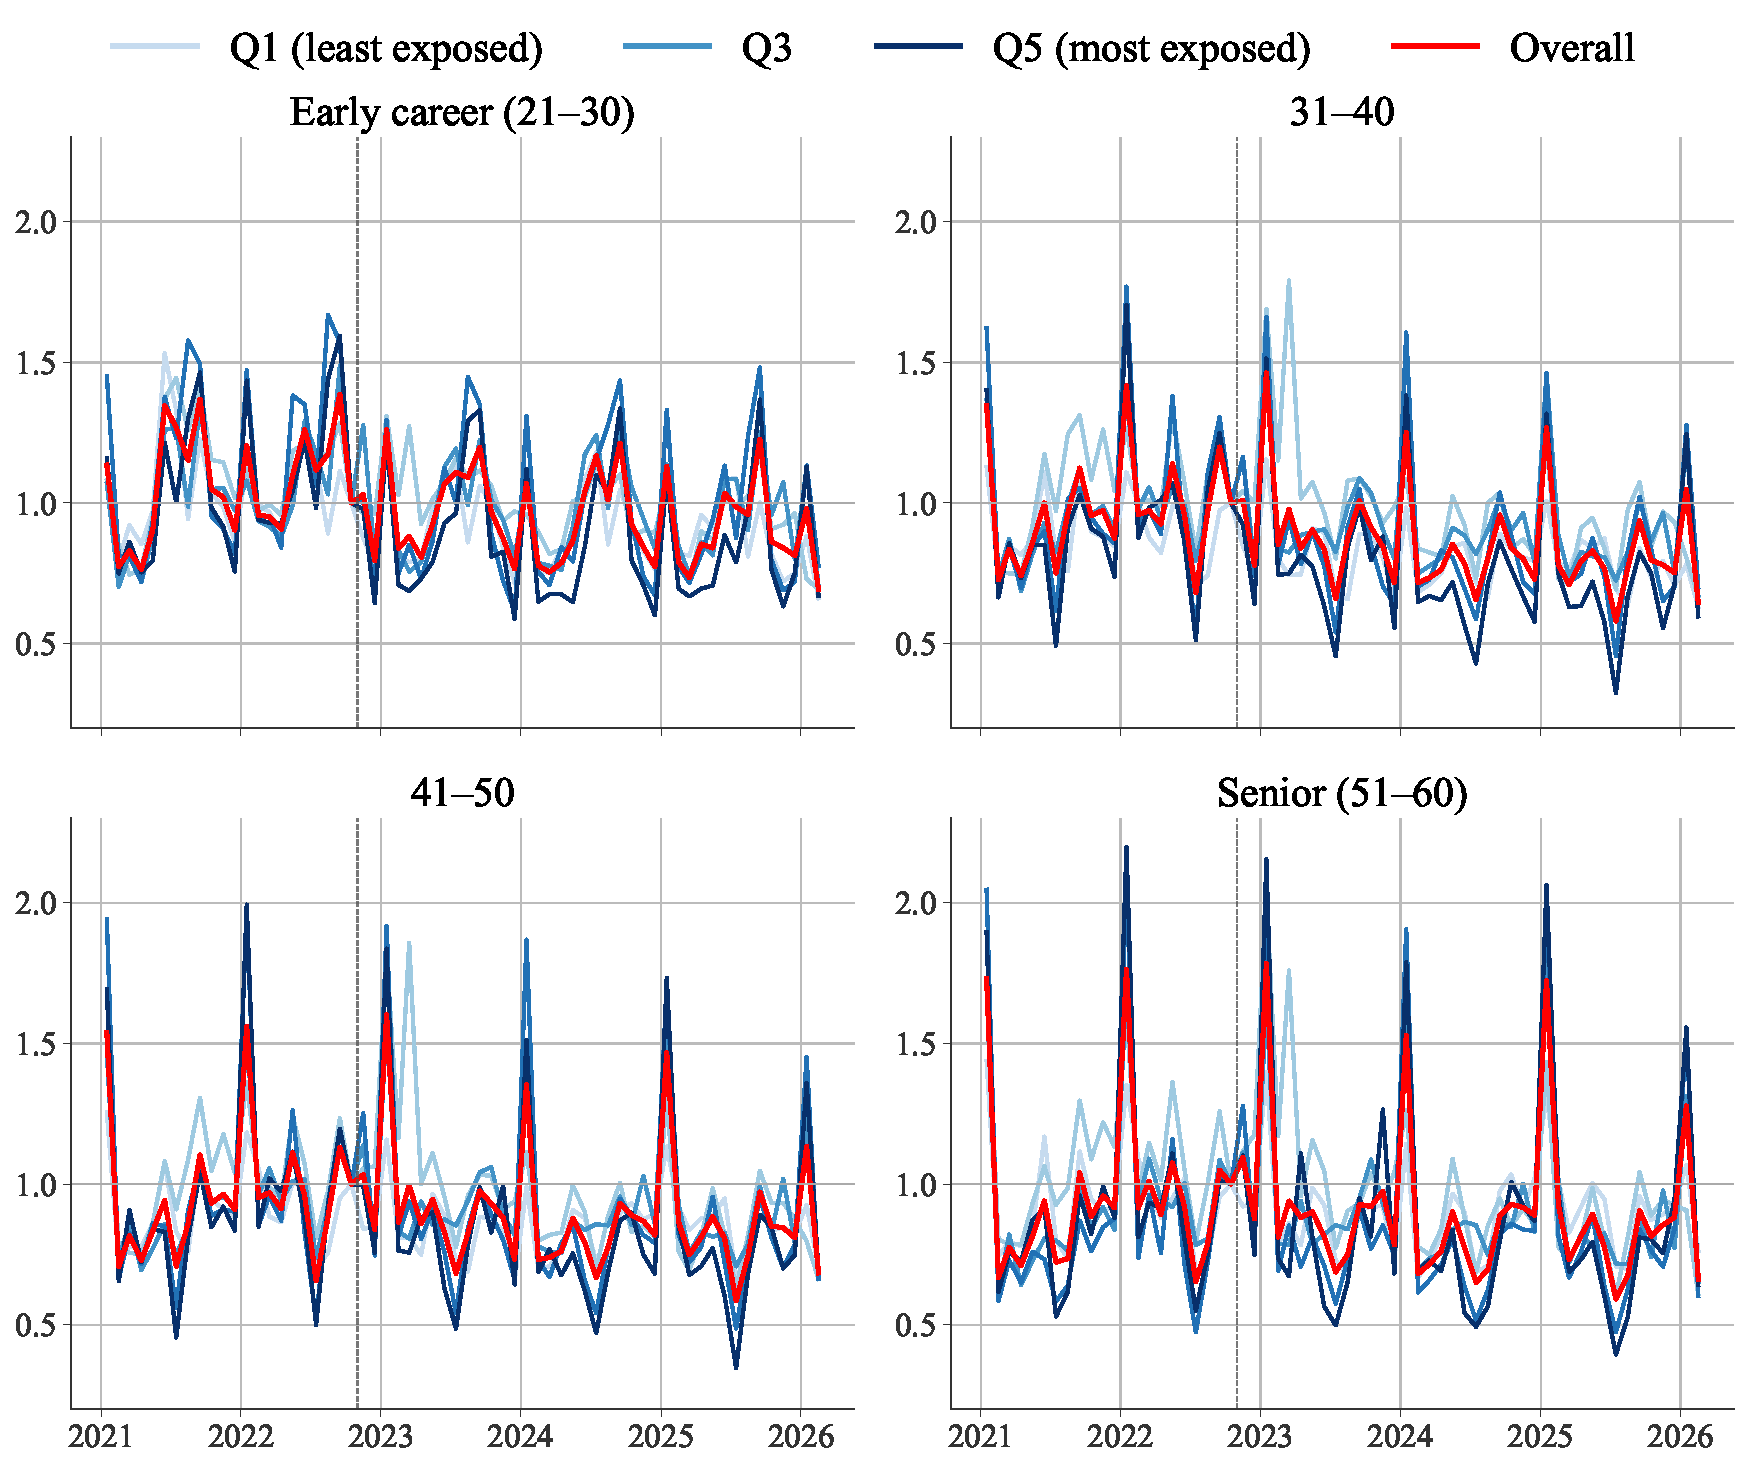
\includegraphics[width=\textwidth]{../analysis/output/figures/figure_ny_jobb_decade_private.pdf}
  \caption{New-hire share by AI-exposure quintile and decade age group, private sector.}
  \label{fig:nyjobb_by_quintile}
  \begin{minipage}{\textwidth}\footnotesize\textit{Notes:} Mean new-hire share, indexed to October 2022 = 1. Occupations are ranked by the Eloundou et al.\ exposure score.\end{minipage}
\end{figure}

\begin{figure}[htbp]
  \centering
  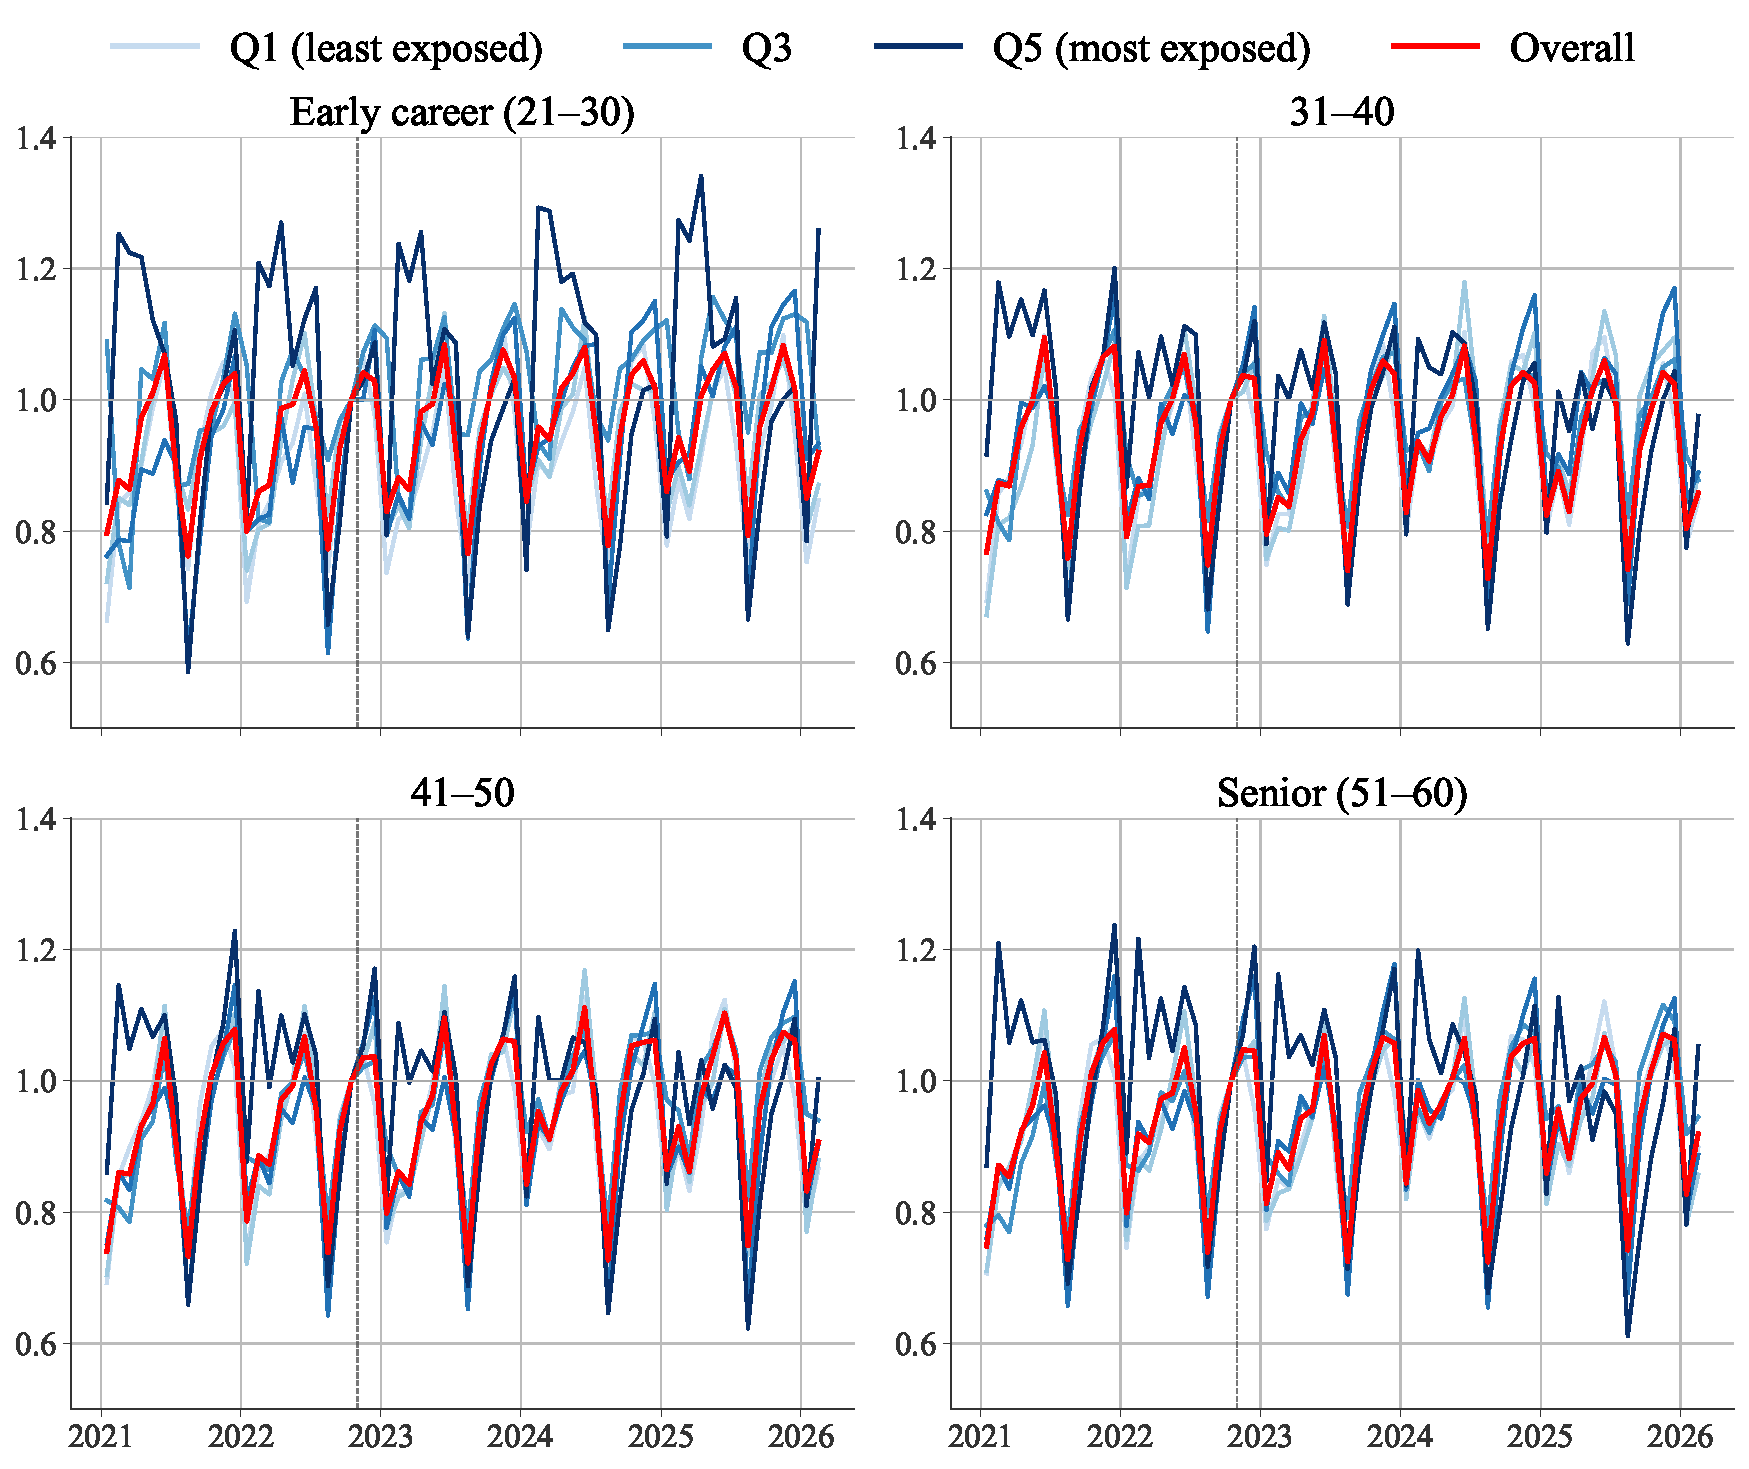
\includegraphics[width=\textwidth]{../analysis/output/figures/figure_overtid_timer_decade_private.pdf}
  \caption{Overtime hours by AI-exposure quintile and decade age group, private sector.}
  \label{fig:overtid_by_quintile}
  \begin{minipage}{\textwidth}\footnotesize\textit{Notes:} Mean overtime hours, indexed to October 2022 = 1. Occupations are ranked by the Eloundou et al.\ exposure score.\end{minipage}
\end{figure}

\begin{figure}[htbp]
  \centering
  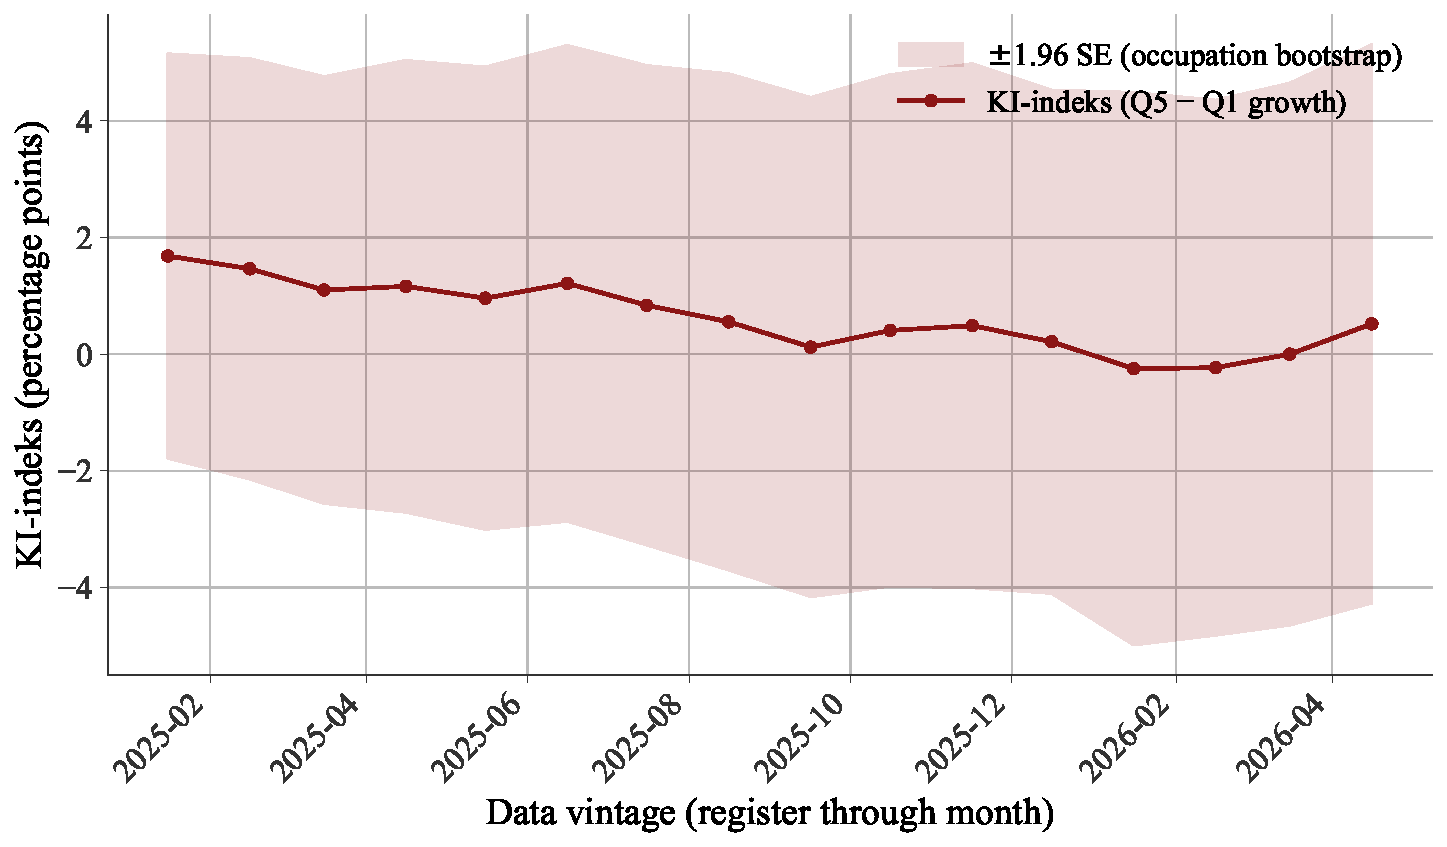
\includegraphics[width=0.85\textwidth]{../analysis/output/figures/figure_recursive_kiindeks_ci.pdf}
  \caption{Real-time reliability of the dashboard headline (``KI-indeks''), re-estimated on expanding data vintages.}
  \label{fig:recursive_kiindeks}
  \begin{minipage}{\textwidth}\footnotesize\textit{Notes:} The dashboard headline is the relative employment growth of the most- versus least-exposed quintile over the most recent three months relative to October 2022, pooled over private-sector workers aged 21 to 60 and seasonally adjusted (X-11 core with seasonal factors frozen on 2021--2024). Each point re-estimates it from the occupation panel on an expanding window, from data through January 2025 to February 2026. The shaded band is $\pm$1.96 occupation cluster-bootstrap standard errors (1{,}000 replications); the dashboard itself reports no uncertainty. The band spans zero in every vintage.\end{minipage}
\end{figure}


% =============================================================================
\clearpage
\phantomsection
\addcontentsline{toc}{section}{Appendix B: Brynjolfsson et al.\ Replication}
\section*{Appendix B: Brynjolfsson et al.\ (2025) Replication}\label{app:bcc}
\setcounter{figure}{0}
\renewcommand{\thefigure}{B\arabic{figure}}
\setcounter{table}{0}
\renewcommand{\thetable}{B\arabic{table}}

We replicate the design of \citet{brynjolfsson2025} on Norwegian register data, on the exact early-career definition used in the cross-country literature. Workers are placed in six age bins (22--25, 26--30, 31--34, 35--40, 41--49, 50--55) that match their 22--25 early-career definition, employment is indexed to October 2022, and occupations are ranked by the Eloundou GPT-4 quintile. The event study (Figure~\ref{fig:bcc_es}) uses the balanced-panel construction of their paper: full-time private-sector workers in foretak with at least 10 workers in each age group every month and at least 100 worker-months per firm-quintile-age cell, a sample smaller and more concentrated in larger firms than the main analysis. The descriptive figures (Figures~\ref{fig:bcc_occ}, \ref{fig:bcc_eloundou}, \ref{fig:bcc_handa} and~\ref{fig:bcc_comp}) instead use all full-time private-sector workers in these age bins, without the firm-balancing restriction; being narrower than the population series in the main text, their raw series move more.

Figure~\ref{fig:bcc_es} reports the Poisson event study. For workers aged 22--25 the post-October-2022 average gap is small, about 3 log points, but it masks a clear time profile: the most-exposed and least-exposed quintiles track each other through early 2025, and from spring 2025 the most-exposed quintile falls below, with the gap widening to about 35 log points by February 2026. This widening rests on the final ten months of data, the confidence intervals are wide, and the joint pre-trend test rejects parallel trends, so it is an emerging pattern rather than an identified effect. The recent gap exceeds the 15 log points \citet{brynjolfsson2025} report for the United States, but the US gap opened earlier and over a far larger sample. The descriptive series behind the replication appear in Figures~\ref{fig:bcc_occ}, \ref{fig:bcc_eloundou}, \ref{fig:bcc_handa} and~\ref{fig:bcc_comp}: selected occupations, the Eloundou exposure quintiles, the Handa usage split, and cash earnings.

\begin{figure}[htbp]
  \centering
  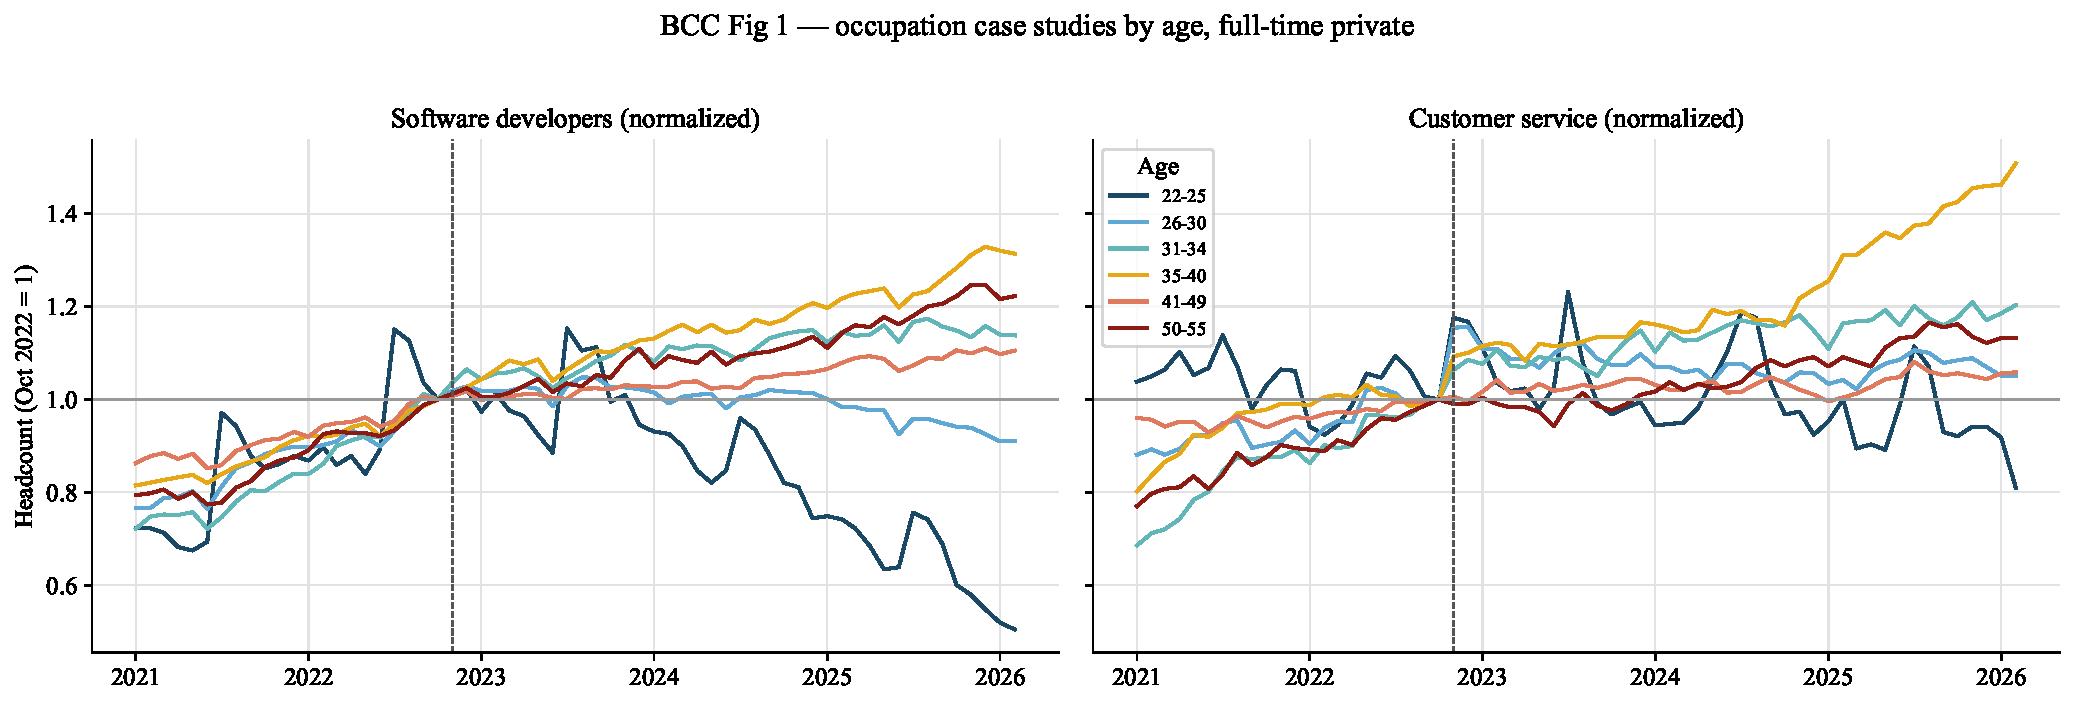
\includegraphics[width=\textwidth]{../analysis-indiv/output/bcc_appendix/fig_bcc_1_occ.pdf}
  \caption{Employment in selected occupations by age group, Brynjolfsson et al.\ replication.}
  \label{fig:bcc_occ}
  \begin{minipage}{\textwidth}\footnotesize\textit{Notes:} Employment indexed to October 2022 = 1, by age group, for software developers (ISCO-08 2512) and customer service (4222). Full-time private-sector workers (descriptive sample, without the event study's firm-balancing restriction).\end{minipage}
\end{figure}

\begin{figure}[htbp]
  \centering
  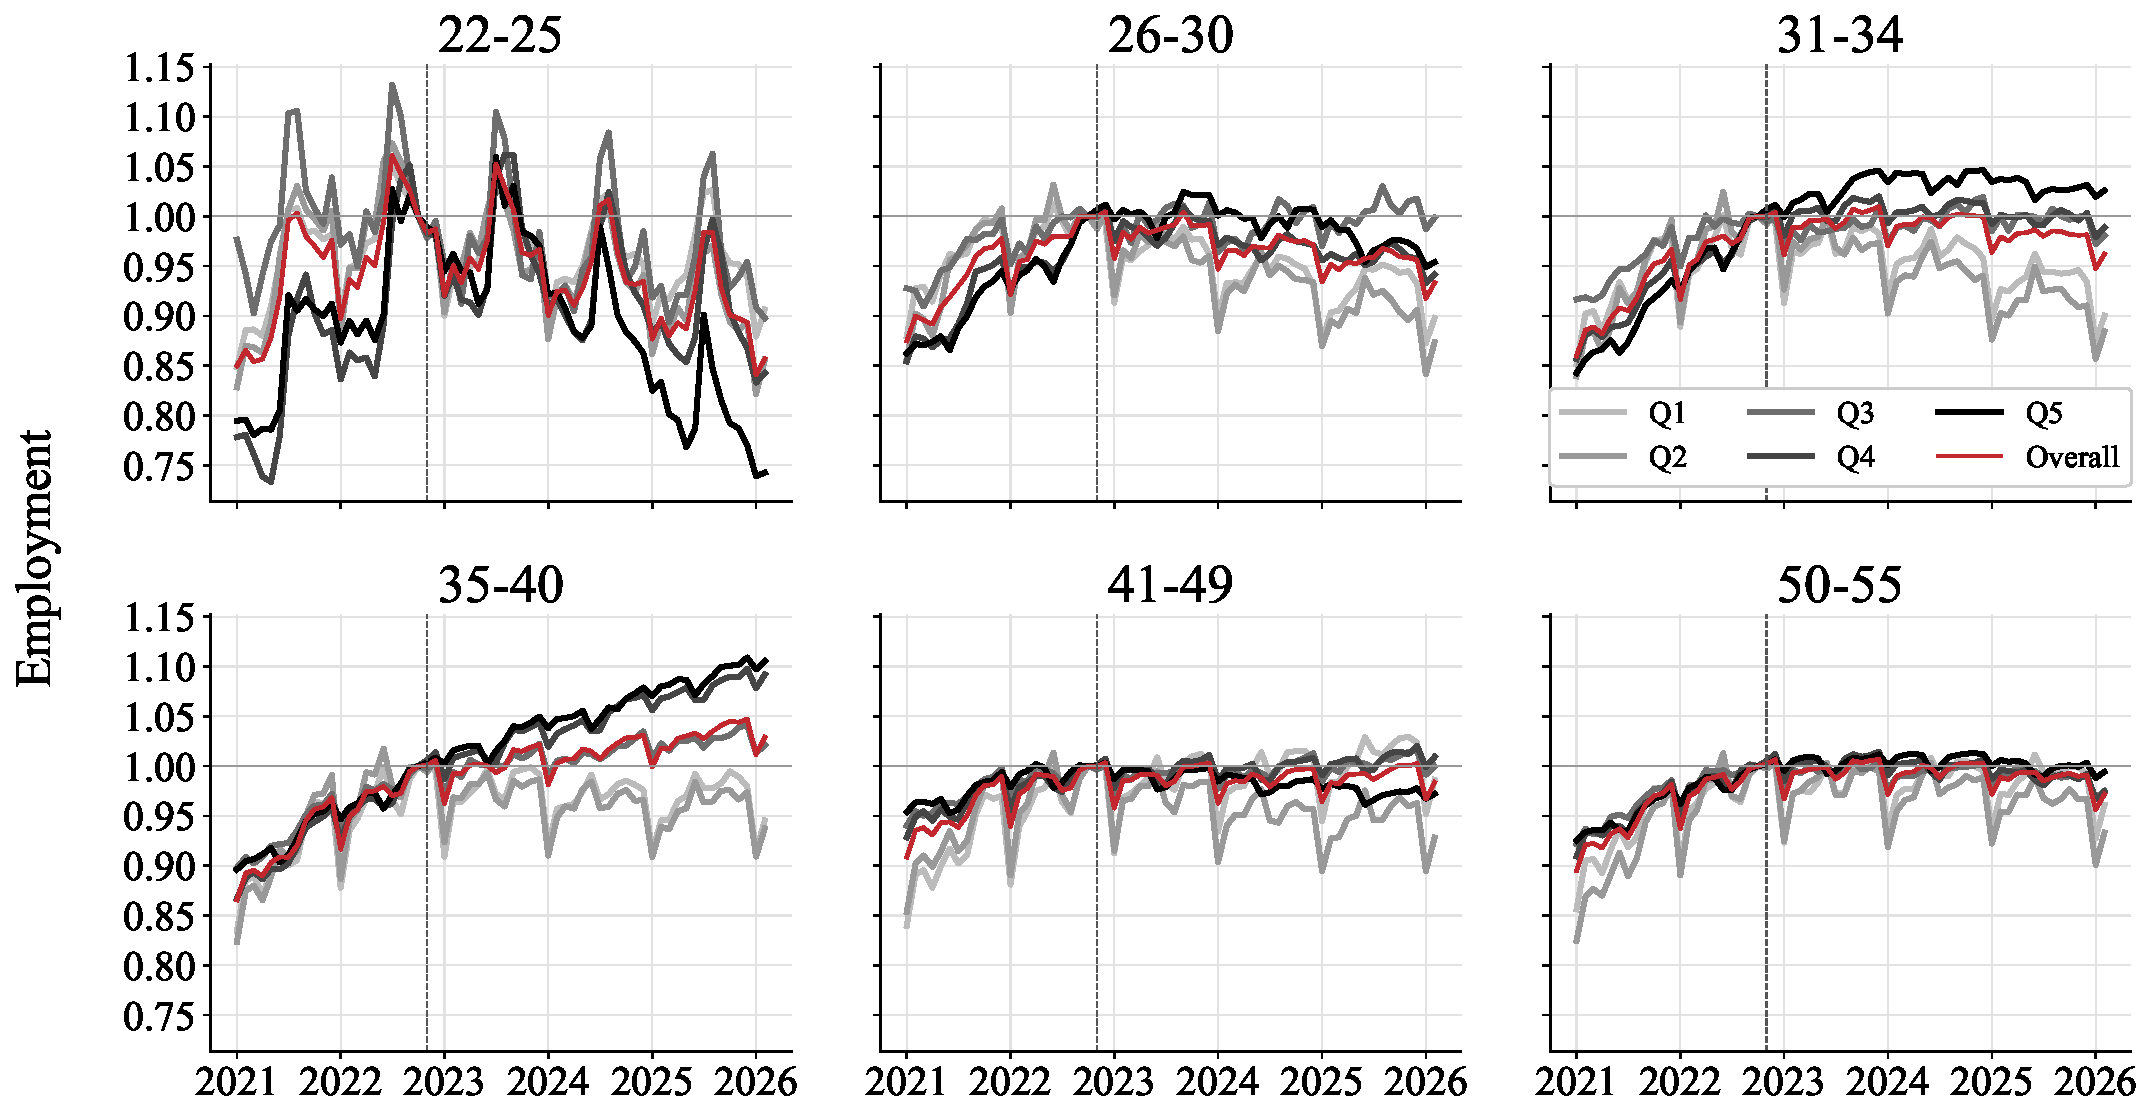
\includegraphics[width=\textwidth]{../analysis-indiv/output/bcc_appendix/fig_bcc_2_eloundou.pdf}
  \caption{Employment by Eloundou exposure quintile and age group, Brynjolfsson et al.\ replication.}
  \label{fig:bcc_eloundou}
  \begin{minipage}{\textwidth}\footnotesize\textit{Notes:} Employment indexed to October 2022 = 1, by Eloundou GPT-4 quintile within each age group, with a pooled overall line. Full-time private-sector workers (descriptive sample, without the event study's firm-balancing restriction).\end{minipage}
\end{figure}

\begin{figure}[htbp]
  \centering
  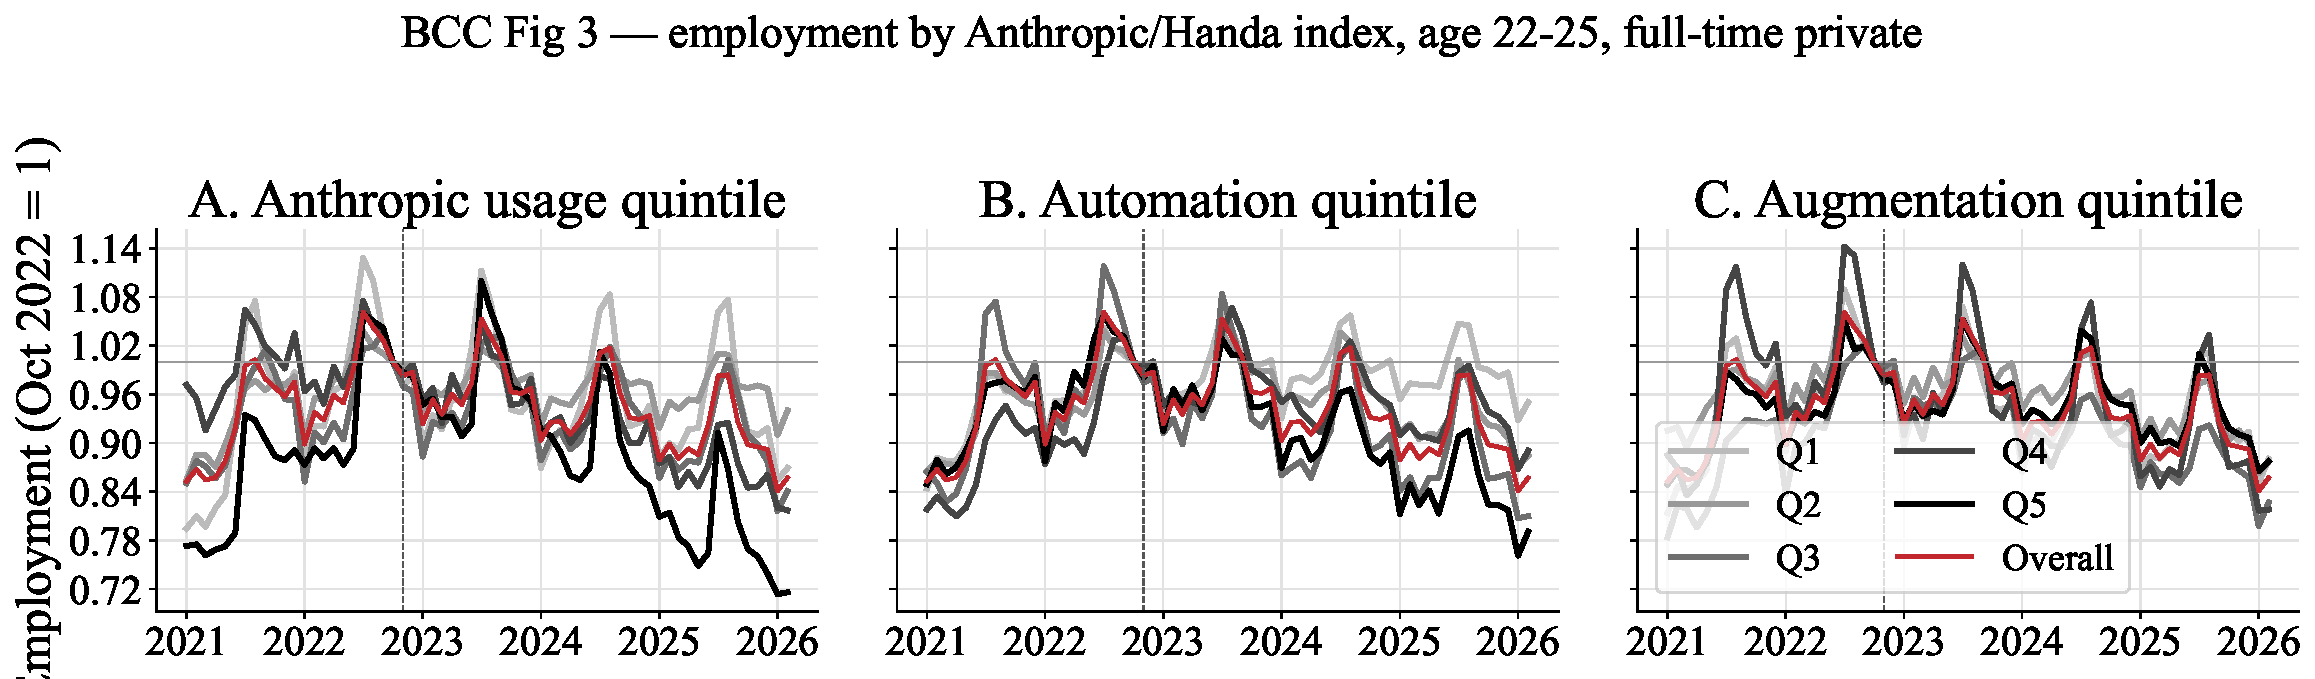
\includegraphics[width=\textwidth]{../analysis-indiv/output/bcc_appendix/fig_bcc_3_handa.pdf}
  \caption{Employment by Handa usage, automation, and augmentation quintile, ages 22--25.}
  \label{fig:bcc_handa}
  \begin{minipage}{\textwidth}\footnotesize\textit{Notes:} Employment indexed to October 2022 = 1 for workers aged 22--25, by Handa et al.\ usage, automation, and augmentation quintile, with a pooled overall line.\end{minipage}
\end{figure}

\begin{figure}[htbp]
  \centering
  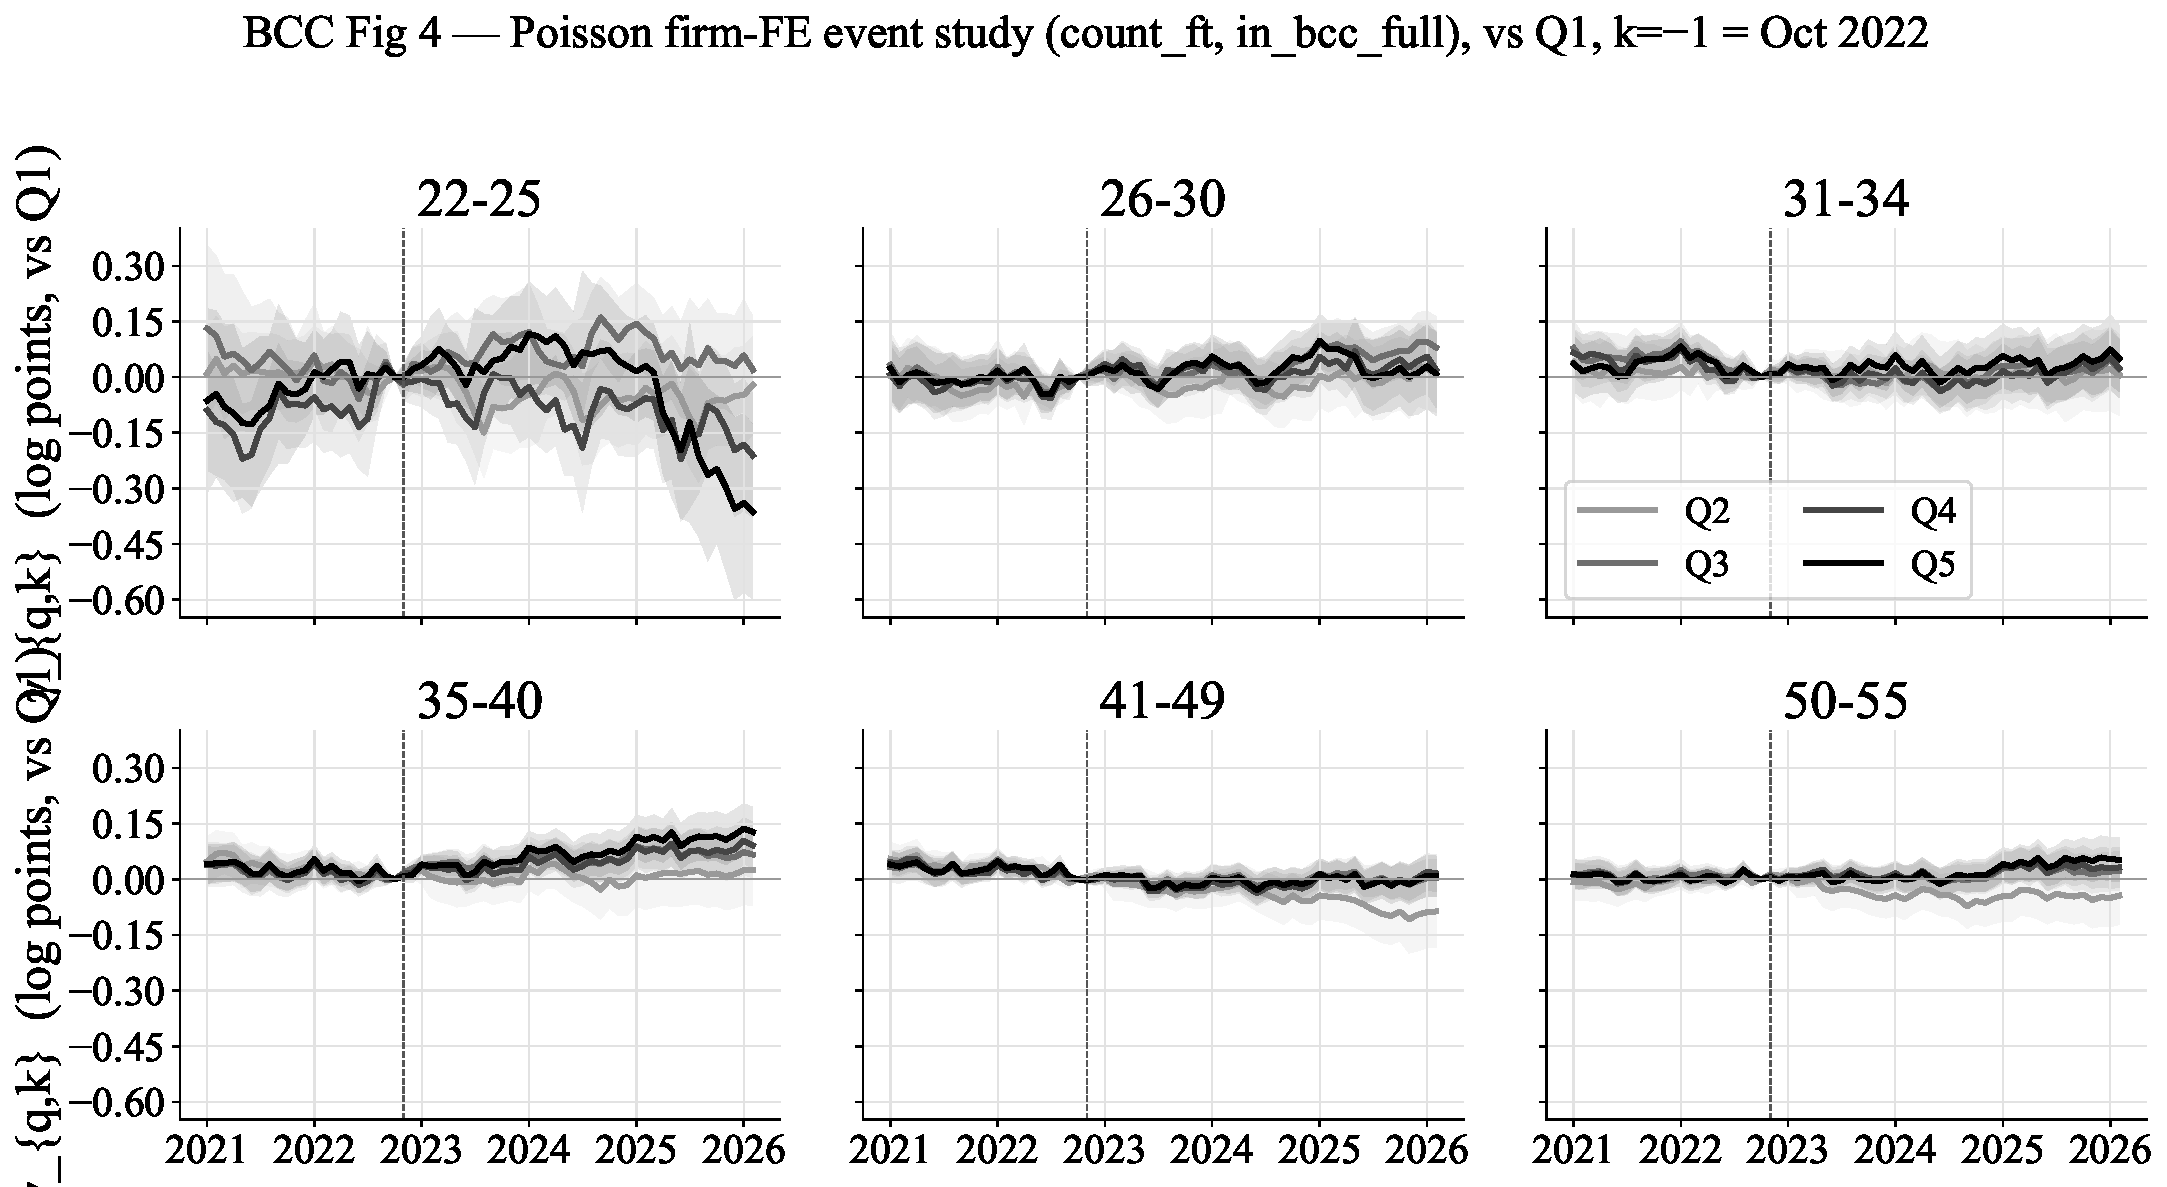
\includegraphics[width=\textwidth]{../analysis-indiv/output/bcc_appendix/fig_bcc_4_es.pdf}
  \caption{Poisson event-study coefficients, most versus least exposed quintile, by age group.}
  \label{fig:bcc_es}
  \begin{minipage}{\textwidth}\footnotesize\textit{Notes:} Q5-vs-Q1 Poisson event-study coefficients, in log points, by six age bins from 22--25 to 50--55, relative to October 2022. Firm fixed effects; standard errors clustered at the firm. Shaded bands: 95\% confidence intervals. Sample 2021m1--2026m2. Dashed line marks the November 2022 ChatGPT release.\end{minipage}
\end{figure}

For the 22--25 event study, we run the same honest difference-in-differences sensitivity analysis as for the main 21--30 sample (Section~\ref{sec:regression:robust}), using the Q5-vs-Q1 firm-FE coefficients. The calculation uses the full clustered variance-covariance matrix exported from the secure server. Even under exact parallel trends ($\bar{M}=0$), the conventional interval includes zero (Table~\ref{tab:honest_did_bcc}), and the breakdown value is zero: the late-opening 22--25 gap remains too imprecise to distinguish from zero in the firm-FE design.

\begin{table}[htbp]
  \centering
  \caption{HonestDiD sensitivity of the Q5-vs-Q1 employment effect, ages 22--25 (Brynjolfsson-style sample).}
  \label{tab:honest_did_bcc}
  \begin{tabular}{lc}
\toprule
Restriction & Robust 95\% CI \\
\midrule
Original ($\bar{M}=0$, parallel trends) & [-0.061, -0.010] \\
$\bar{M}=0.5$ & [-0.822, +0.746] \\
$\bar{M}=1.0$ & [-1.500, +1.500] \\
$\bar{M}=1.5$ & [-1.500, +1.500] \\
$\bar{M}=2.0$ & [-1.500, +1.500] \\
\midrule
Breakdown $\bar{M}$ & 0.00 \\
\bottomrule
\end{tabular}

  \begin{minipage}{\textwidth}\footnotesize\textit{Notes:} Robust 95\% confidence intervals for the average post-ChatGPT Q5-vs-Q1 employment difference, ages 22--25, under the relative-magnitude restriction of \citet{rambachan2023}. Computed from the individual-level firm-FE event-study coefficients and their full clustered variance-covariance matrix, exported from the secure server; months are aggregated to quarters and the target is the average post-ChatGPT effect. $\bar{M}=0$ is exact parallel trends; ``Breakdown'' is the largest $\bar{M}$ for which the interval excludes zero.\end{minipage}
\end{table}

\begin{figure}[htbp]
  \centering
  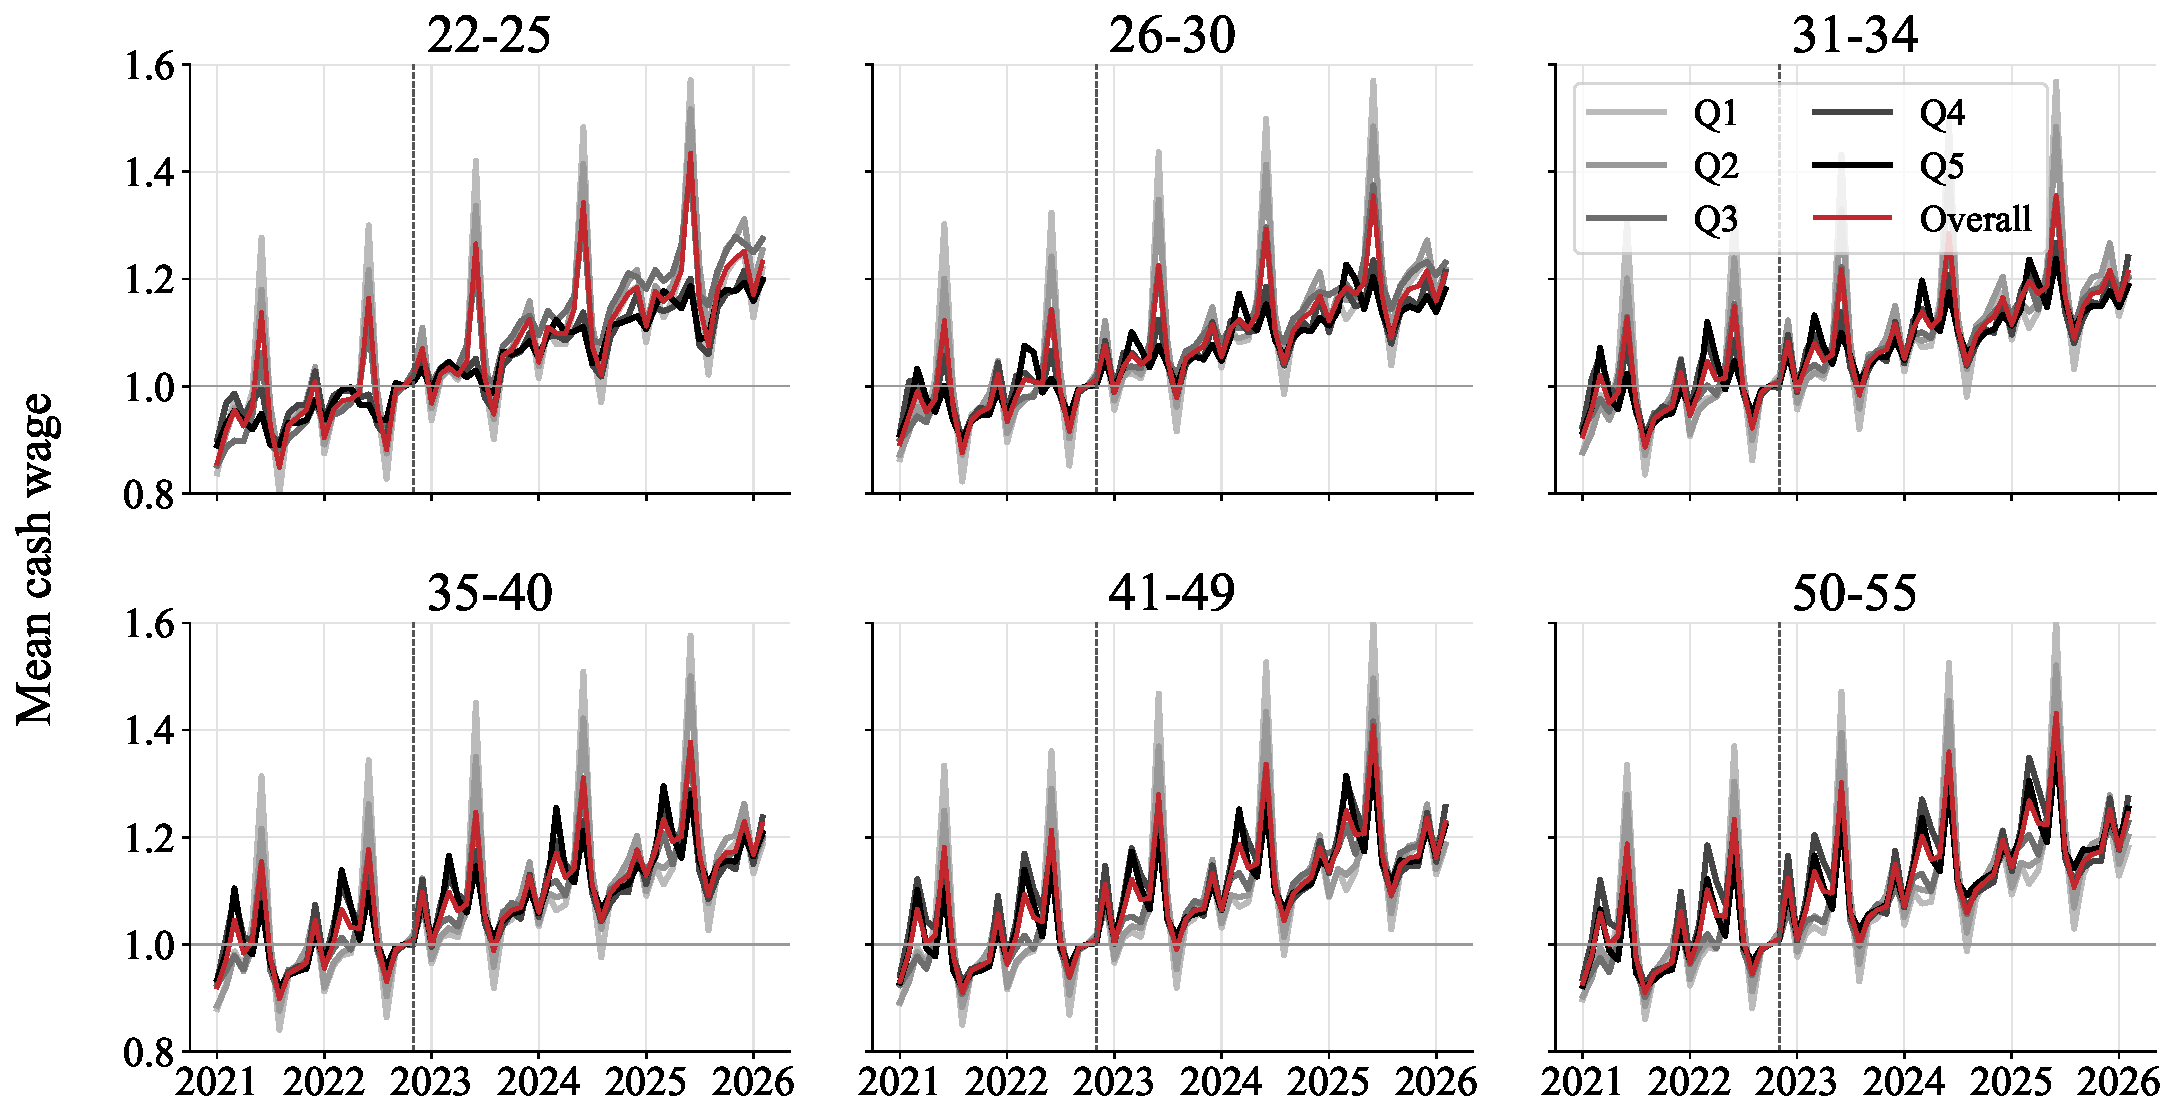
\includegraphics[width=\textwidth]{../analysis-indiv/output/bcc_appendix/fig_bcc_5_comp.pdf}
  \caption{Mean cash earnings by Eloundou exposure quintile and age group, Brynjolfsson et al.\ replication.}
  \label{fig:bcc_comp}
  \begin{minipage}{\textwidth}\footnotesize\textit{Notes:} Mean monthly cash earnings indexed to October 2022 = 1, by Eloundou GPT-4 quintile within each age group, with a pooled overall line. Full-time private-sector workers (descriptive sample, without the event study's firm-balancing restriction).\end{minipage}
\end{figure}

\end{document}
